\chapter{Strutture succinte}
\section{Abstract data types}
Gli \textit{abstract data type} sono tipi di dati descritti dal loro comportamento: un esempio è
l'ADT \texttt{stack<T>}, il quale è dotato di alcune operazioni inerenti al tipo
stesso, chiamate \textbf{primitive}:
\begin{lstlisting}
  bool  isEmpty()
  T     top()
  void  pop()
  void  push(T)
\end{lstlisting}
Il cosa facciano i metodi si può descrivere in molti modi: si può
utilizzare un metodo discorsivo, spiegando a parole, o utilizzare un metodo
analitico:
$$
	\forall S, s.push(x).top() = x
$$
(nonostante la notazione impropria dovuta alla signatura delle funzioni);
$$
	\forall S, s.isEmpty() \implies S.push(x).pop().isEmpty()
$$
Una volta descritto un ADT è necessario implementarlo, ossia costruire effettivamente
una struttura che implementa le primitive rispettandone la descrizione. Chiaramente,
vi sono molte implementazioni diverse che soddisfano le richieste
ma hanno \textit{costi} diversi, sia in tempo che in spazio. Siamo interessati
ad alcuni ADT e relative implementazioni che utilizzano poco tempo e spazio.
Ogni ADT ha associato un concetto di \textit{taglia}, che rappresenta genericamente
la grandezza di un'istanza: nel caso dello stack, la taglia sarebbe il numero
di elementi presenti sulla pila.

\subsection{Teoria dell'informazione}
Per poter caratterizzare le implementazioni degli ADT in base allo
spazio che occupano è necessario introdurre alcuni concetti della teoria
dell'informazione, i quali discendono dai Teoremi di Shannon,
sommariamente riassumibili nel seguente teorema.

\begin{theorem}[della codifica della sorgente]
	\label{thm:shannon}
	Per codificare $v$ valori servono in media $\log_2(v)$ bit.
\end{theorem}

Per esempio, immaginiamo di dover codificare un'immagine $100\times100$ pixel
in bianco e nero. Le immagini possibili sono $2^{10000}$: per codificare
queste immagini servono in media $10000$ bit. In effetti, la
rappresentazione banale che rappresenta ogni pixel, utilizza esattamente
$10000$ bit e non potrebbe usarne di meno! Usandone, per esempio, solo
$9000$, alcune immagini diverse avrebbero la stessa rappresentazione.

Questo teorema vale anche per rappresentazioni di dimensione
variabile, ossia vale anche per codifiche: si supponga di avere un
algoritmo in grado di comprimere tre immagini ognuna in $100$ bit.
La conseguenza di questo teorema è che ci saranno delle altre immagini che
utilizzeranno più di $10000$ bit, in modo che la media rimanga $10000$.

In generale, dati $v$ valori rappresentabili con $x_1, x_2, \cdots, x_v$ bit
rispettivamente; il Teorema afferma che
$$
	\frac{\sum_{i} x_i}{v} \geq \log_2(v)
$$

In realtà il \cref{thm:shannon} dice di più, ossia che è possibile creare un
sistema di compressione per i $v$ valori utilizzando un numero di bit medio
tra $[\log_2(v), 1 + \log_2(v))$, assumendo che tutti i $v$ valori siano
equiprobabili\footnote{
	\cite{shannon_1948} è il lavoro di C. Shannon che ha dato vita al campo della
	teoria dell'informazione; un approccio più moderno è \cite{cover_2006}. }.

Ci confronteremo spesso con questo \textbf{information-theoretical lower bound}:
immaginiamo tutte le possibili istanze $v_i$ di ADT di taglia $i$;
per esempio, uno stack con valori in $\{0, 1, \cdots, 9\}$;
lo stack di taglia $0$ è lo stack vuoto, gli stack
di taglia $1$ sono le $10$ istanze stack che contengono solo $1$, solo $2$, e così via,
mentre gli stack di taglia $2$ sono $10^2$; in generale uno stack
di taglia $n$ ha $10^n$ valori. Il Teorema afferma che in media servono
$\log_2{10^n} = n \log_2(10) \approx 4n$ bit per rappresentare uno stack
con valori in $\{0, 1, \cdots, 9\}$: sappiamo quindi che
\textit{nessuna implementazione} può utilizzare, in media, meno di
$Z_n =n \log_2(10)$ bit, l'information-theoretical lower bound per
rappresentare stack di taglia $n$ con valori in $\{0, 1, \cdots, 9\}$.

Ipotizziamo di avere una struttura che utilizza in media $D_n \geq Z_n$ bit:
esiste un tradeoff tra quanto \textit{compatta} è la struttura e quanto
tempo è necessario per eseguire le funzioni primitive.
Esistono sistemi di compressione che ignorano completamente il problema:
ad esempio, comprimendo un oggetto con l'algoritmo \texttt{tz2}, non si può
utilizzare l'oggetto compresso come la sua rappresentazione non compressa
per eseguire le primitive su di esso! Noi siamo interessati a strutture
compresse - rappresentano i dati in maniera efficiente rispetto allo spazio -
e con primitive efficienti tanto quanto un'implementazione non compressa.

Definiamo quindi delle classificazioni delle implementazioni in base al rapporto
tra l'effettivo utilizzo di spazio (in media) e l'indice $Z_n$:
un'implementazione dell'ADT è chiamata \textbf{implicita} se occupa un numero
di bit $D_n = Z_n + O(1)$, \textbf{succinta} se occupa un numero di bit
$D_n = Z_n + o(Z_n)$ e \textbf{compatta} se $D_n = O(Z_n)$; tutto questo sempre
notando che le primitive devono essere efficienti tanto quanto quelle definite
su strutture non compresse.

\section{Strutture di rango e selezione}
Questi ADT sono definiti da un vettore $\mathbb{b} \in 2^n$ con due primitive:
$$
	\mathbf{rank}_b: \mathbb{N} \rightarrow \mathbb{N}
$$
$$
	\mathbf{select}_b: \mathbb{N} \rightarrow \mathbb{N}
$$
tali che:
$$
	\forall p \leq n ~~ \mathbf{rank}_b(p) = |\{i | i < p \land b_i = 1\}|
$$
$$
	\forall k \leq n ~~ \mathbf{select}_b(k) =\max \{p | \mathbf{rank}_b(p) \leq k\}
$$
Quindi, per esempio, per un $\mathbf{b} = [0 1 1 0 1 0 1]$ si hanno due
tabelle di rank e select come in \cref{table:rank_sel}.

\begin{table}[ht]
	\centering

	\begin{subtable}{0.45\textwidth}
		\centering
		\begin{tabular}{c|c}
			$p$ & $\mathbf{rank}_b(p)$ \\ \hline
			0   & 0                    \\
			1   & 0                    \\
			2   & 1                    \\
			3   & 2                    \\
			4   & 2                    \\
			5   & 3                    \\
			6   & 3                    \\
			7   & 4
		\end{tabular}
		\caption{$\mathbf{rank}_b(p)$}
	\end{subtable}
	\begin{subtable}{0.45\textwidth}
		\centering
		\begin{tabular}{c|c}
			$k$      & $\mathbf{select}_b(p)$ \\ \hline
			0        & 1                      \\
			1        & 2                      \\
			2        & 3                      \\
			3        & 6                      \\
			4        & 7                      \\
			5        & 7                      \\
			$\cdots$ & 7                      \\
		\end{tabular}
		\caption{$\mathbf{select}_b(p)$}
	\end{subtable}
	\caption{Tabelle per $\mathbf{b}$.}
	\label{table:rank_sel}
\end{table}
Rank e select sono funzioni inverse in un senso molto stretto, ciò vale che
$$
	\forall k ~~ \mathbf{rank}_b(\mathbf{select}_b(k)) = k
$$
mentre l'inverso, ossia applicare select a rank, si ottiene una proprietà
diversa:
$$
	\forall p ~~ \mathbf{select}_b(\mathbf{rank}_b(p)) \geq p
$$
proprio grazie a quest'ultima proprietà è possibile dedurre la struttura sottostante,
nel senso che è possibile capire dove siano gli $0$ e gli $1$ in $\mathbf{b}$.

\subsection{Struttura di Jacobson per il rango}
\subsubsection{Four-russians trick}
L'implementazione dell'ADT rank di Jacobson
utilizza il ``four-russians trick''. Si immagini di
voler rappresentare una matrice binaria: un modo per farlo potrebbe essere
dividere la matrice in blocchi chiamati \textit{piastrelle} ed enumerare
le possibili piastrelle. Chiaramente, se nella matrice appare ogni possibile
combinazione di piastrella, il guadagno del trucco sarà nullo.
Se, invece, la matrice è molto ripetitiva, le piastrelle possibili da ricordare saranno
poche e basterà utilizzare il numero associato alla piastrella per rappresentare
l'intera matrice. Un esempio è in \cref{fig:frtrick}.

% disegno.. 19-11-2021 ... 
\begin{figure}[ht]
	\centering
	\begin{subfigure}{0.32\textwidth}
		\centering
		\tikzset{every picture/.style={line width=0.75pt}} %set default line width to 0.75pt        

		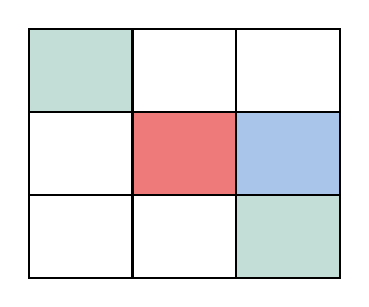
\begin{tikzpicture}[x=0.75pt,y=0.75pt,yscale=-1,xscale=1]
			%uncomment if require: \path (0,300); %set diagram left start at 0, and has height of 300

			%Shape: Rectangle [id:dp005749332004390428] 
			\draw  [fill={rgb, 255:red, 195; green, 222; blue, 215 }  ,fill opacity=1 ] (10,30) -- (60,30) -- (60,70) -- (10,70) -- cycle ;
			%Shape: Rectangle [id:dp7752907448209945] 
			\draw   (60,30) -- (110,30) -- (110,70) -- (60,70) -- cycle ;
			%Shape: Rectangle [id:dp6434156098479539] 
			\draw   (110,30) -- (160,30) -- (160,70) -- (110,70) -- cycle ;
			%Shape: Rectangle [id:dp6511151383263759] 
			\draw   (10,70) -- (60,70) -- (60,110) -- (10,110) -- cycle ;
			%Shape: Rectangle [id:dp12594297400828225] 
			\draw  [color={rgb, 255:red, 0; green, 0; blue, 0 }  ,draw opacity=1 ][fill={rgb, 255:red, 239; green, 122; blue, 122 }  ,fill opacity=1 ] (60,70) -- (110,70) -- (110,110) -- (60,110) -- cycle ;
			%Shape: Rectangle [id:dp07170680173867716] 
			\draw  [fill={rgb, 255:red, 169; green, 198; blue, 234 }  ,fill opacity=1 ] (110,70) -- (160,70) -- (160,110) -- (110,110) -- cycle ;
			%Shape: Rectangle [id:dp016792670255308284] 
			\draw   (10,110) -- (60,110) -- (60,150) -- (10,150) -- cycle ;
			%Shape: Rectangle [id:dp40735665999968684] 
			\draw   (60,110) -- (110,110) -- (110,150) -- (60,150) -- cycle ;
			%Shape: Rectangle [id:dp5192196869257351] 
			\draw  [fill={rgb, 255:red, 195; green, 222; blue, 215 }  ,fill opacity=1 ] (110,110) -- (160,110) -- (160,150) -- (110,150) -- cycle ;
		\end{tikzpicture}
		\caption{Tabella iniziale. Ogni riquadro contiene $5$ bit.}
	\end{subfigure}
	\begin{subfigure}{0.32\textwidth}
		\centering

		\tikzset{every picture/.style={line width=0.75pt}} %set default line width to 0.75pt        

		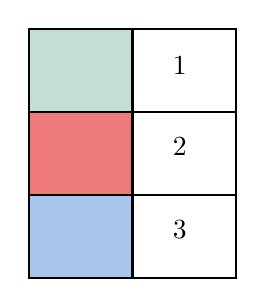
\begin{tikzpicture}[x=0.75pt,y=0.75pt,yscale=-1,xscale=1]
			%uncomment if require: \path (0,300); %set diagram left start at 0, and has height of 300

			%Shape: Rectangle [id:dp7804092113436614] 
			\draw  [fill={rgb, 255:red, 195; green, 222; blue, 215 }  ,fill opacity=1 ] (200,50) -- (250,50) -- (250,90) -- (200,90) -- cycle ;
			%Shape: Rectangle [id:dp023528268951144793] 
			\draw  [fill={rgb, 255:red, 239; green, 122; blue, 122 }  ,fill opacity=1 ] (200,90) -- (250,90) -- (250,130) -- (200,130) -- cycle ;
			%Shape: Rectangle [id:dp43332731525643986] 
			\draw  [fill={rgb, 255:red, 169; green, 198; blue, 234 }  ,fill opacity=1 ] (200,130) -- (250,130) -- (250,170) -- (200,170) -- cycle ;
			%Shape: Rectangle [id:dp31985072077933197] 
			\draw   (250,50) -- (300,50) -- (300,90) -- (250,90) -- cycle ;

			%Shape: Rectangle [id:dp6876058724781219] 
			\draw   (250,90) -- (300,90) -- (300,130) -- (250,130) -- cycle ;

			%Shape: Rectangle [id:dp9303810523957489] 
			\draw   (250,130) -- (300,130) -- (300,170) -- (250,170) -- cycle ;

			% Text Node
			\draw (268,141) node [anchor=north west][inner sep=0.75pt]   [align=left] {3};
			% Text Node
			\draw (268,101) node [anchor=north west][inner sep=0.75pt]   [align=left] {2};
			% Text Node
			\draw (268,62) node [anchor=north west][inner sep=0.75pt]   [align=left] {1};
		\end{tikzpicture}
		\caption{Enumerazione di sottomatrici.}
	\end{subfigure}
	\begin{subfigure}{0.32\textwidth}
		\centering
		\tikzset{every picture/.style={line width=0.75pt}} %set default line width to 0.75pt        

		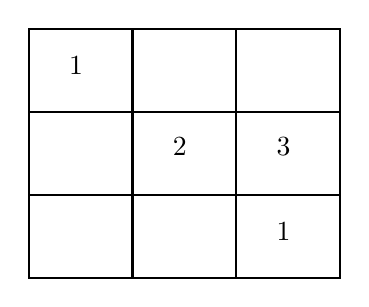
\begin{tikzpicture}[x=0.75pt,y=0.75pt,yscale=-1,xscale=1]
			%uncomment if require: \path (0,300); %set diagram left start at 0, and has height of 300

			%Shape: Rectangle [id:dp021688033849312616] 
			\draw   (295,78) -- (345,78) -- (345,118) -- (295,118) -- cycle ;
			%Shape: Rectangle [id:dp6593678571435228] 
			\draw   (345,78) -- (395,78) -- (395,118) -- (345,118) -- cycle ;
			%Shape: Rectangle [id:dp05373113383793526] 
			\draw  [fill={rgb, 255:red, 195; green, 222; blue, 215 }  ,fill opacity=0 ] (245,118) -- (295,118) -- (295,158) -- (245,158) -- cycle ;
			%Shape: Rectangle [id:dp881184835248234] 
			\draw  [fill={rgb, 255:red, 195; green, 222; blue, 215 }  ,fill opacity=0 ] (245,158) -- (295,158) -- (295,198) -- (245,198) -- cycle ;
			%Shape: Rectangle [id:dp40942537357979314] 
			\draw   (295,158) -- (345,158) -- (345,198) -- (295,198) -- cycle ;
			%Shape: Rectangle [id:dp4268873556029348] 
			\draw   (245,78) -- (295,78) -- (295,118) -- (245,118) -- cycle ;

			%Shape: Rectangle [id:dp9673334799284516] 
			\draw   (345,158) -- (395,158) -- (395,198) -- (345,198) -- cycle ;

			%Shape: Rectangle [id:dp06125848702433001] 
			\draw   (295,118) -- (345,118) -- (345,158) -- (295,158) -- cycle ;

			%Shape: Rectangle [id:dp6270788142678815] 
			\draw   (345,118) -- (395,118) -- (395,158) -- (345,158) -- cycle ;


			% Text Node
			\draw (363,129) node [anchor=north west][inner sep=0.75pt]   [align=left] {3};
			% Text Node
			\draw (313,129) node [anchor=north west][inner sep=0.75pt]   [align=left] {2};
			% Text Node
			\draw (363,170) node [anchor=north west][inner sep=0.75pt]   [align=left] {1};
			% Text Node
			\draw (263,90) node [anchor=north west][inner sep=0.75pt]   [align=left] {1};


		\end{tikzpicture}
		\caption{Matrice risultante dopo l'applicazione del \textit{four-russians trick}.}
	\end{subfigure}
	\caption{Trucco dei quattro russi.}
	\label{fig:frtrick}
\end{figure}

% lezione 17 - 24-11-2021
\subsubsection{Implementazione}
Il vettore $\mathbf{b}$  di $n$ bit viene quindi diviso in blocchi della
stessa lunghezza, chiamati \textit{superblocchi}, di lunghezza
$\log_2(n)^2$. Ogni superblocco viene
diviso a sua volta in blocchi più piccoli, di lunghezza $\frac{1}{2} \log_2(n)$,
come rappresentato in \cref{fig:jrank}.
\begin{figure}[ht]
	\centering
	\tikzset{every picture/.style={line width=0.75pt}} %set default line width to 0.75pt        

	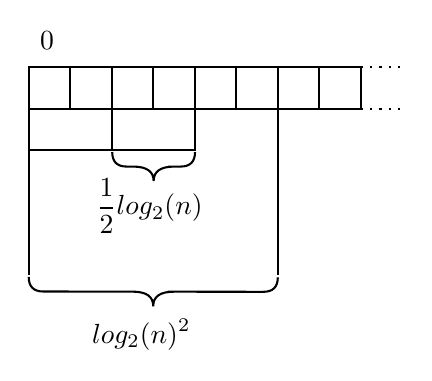
\begin{tikzpicture}[x=0.75pt,y=0.75pt,yscale=-1,xscale=1]
		%uncomment if require: \path (0,300); %set diagram left start at 0, and has height of 300

		%Shape: Brace [id:dp6738156163571107] 
		\draw   (150,231) .. controls (149.99,235.67) and (152.32,238) .. (156.99,238.01) -- (199.99,238.07) .. controls (206.66,238.08) and (209.99,240.41) .. (209.98,245.08) .. controls (209.99,240.41) and (213.32,238.09) .. (219.99,238.1)(216.99,238.09) -- (262.99,238.16) .. controls (267.66,238.17) and (269.99,235.84) .. (270,231.17) ;
		%Straight Lines [id:da0175742846479654] 
		\draw    (150,150) -- (150,230) ;
		%Straight Lines [id:da9565831392918982] 
		\draw    (270,150) -- (270,230) ;
		%Shape: Rectangle [id:dp2322340296066201] 
		\draw   (150,130) -- (170,130) -- (170,150) -- (150,150) -- cycle ;
		%Shape: Rectangle [id:dp44447847120593675] 
		\draw   (170,130) -- (190,130) -- (190,150) -- (170,150) -- cycle ;
		%Shape: Rectangle [id:dp11830121656354553] 
		\draw   (190,130) -- (210,130) -- (210,150) -- (190,150) -- cycle ;
		%Shape: Rectangle [id:dp03816859758995417] 
		\draw   (210,130) -- (230,130) -- (230,150) -- (210,150) -- cycle ;
		%Shape: Rectangle [id:dp9408927207358553] 
		\draw   (230,130) -- (250,130) -- (250,150) -- (230,150) -- cycle ;
		%Shape: Rectangle [id:dp9557419136965325] 
		\draw   (250,130) -- (270,130) -- (270,150) -- (250,150) -- cycle ;
		%Shape: Rectangle [id:dp7039774887247845] 
		\draw   (270,130) -- (290,130) -- (290,150) -- (270,150) -- cycle ;
		%Shape: Rectangle [id:dp3777415956586846] 
		\draw   (290,130) -- (310,130) -- (310,150) -- (290,150) -- cycle ;
		%Shape: Rectangle [id:dp35581942359165963] 
		\draw   (150,150) -- (190,150) -- (190,170) -- (150,170) -- cycle ;
		%Shape: Rectangle [id:dp047912414707197204] 
		\draw   (190,150) -- (230,150) -- (230,170) -- (190,170) -- cycle ;
		%Shape: Brace [id:dp6450376307720747] 
		\draw   (190.22,170.82) .. controls (190.22,175.49) and (192.55,177.82) .. (197.22,177.82) -- (200.17,177.82) .. controls (206.84,177.82) and (210.17,180.15) .. (210.17,184.82) .. controls (210.17,180.15) and (213.5,177.82) .. (220.17,177.82)(217.17,177.82) -- (223.11,177.82) .. controls (227.78,177.82) and (230.11,175.49) .. (230.11,170.82) ;
		%Straight Lines [id:da007337321639370731] 
		\draw  [dash pattern={on 0.84pt off 2.51pt}]  (310,130) -- (330,130) ;
		%Straight Lines [id:da4459939594214508] 
		\draw  [dash pattern={on 0.84pt off 2.51pt}]  (310,150) -- (330,150) ;

		% Text Node
		\draw (179,250) node [anchor=north west][inner sep=0.75pt]   [align=left] {$\displaystyle log_{2}( n)^{2}$};
		% Text Node
		\draw (181,182) node [anchor=north west][inner sep=0.75pt]   [align=left] {$\displaystyle \frac{1}{2} log_{2}( n)$};
		% Text Node
		\draw (154,111.4) node [anchor=north west][inner sep=0.75pt]    {$0$};


	\end{tikzpicture}
	\caption{Divisione di $\textbf{b}$ in superblocchi e blocchi.}
	\label{fig:jrank}
\end{figure}
Per esempio, se $n = 256$, i superblocchi avranno lunghezza
$\log_2(256)^2 = 8^2 = 64$ bit e saranno $256/64 = 4$, mentre i
blocchi interni saranno $\frac{1}{2}\log_2(256) = \frac{1}{2}8 = 4$ bit e saranno
$64/4 = 16$ per superblocco, $16*4 = 64$ in totale.
In questo esempio, i possibili blocchi sono $2^4 = 16$ e, in generale,
siccome i blocchi hanno lunghezza $\frac{1}{2} \log_2(n)$, sono
$$
	2^{\frac{1}{2}\log_2(n)} = (2^{\log_2(n)})^{\frac{1}{2}} =  \sqrt{n}
$$
Se volessimo memorizzare la funzione di rank per un singolo blocco,
costruiremmo una tabella di $\frac{1}{2}\log_2(n)$ righe e per ognuna
di queste bisognerebbe salvare il numero di $1$ presenti nel blocco fino a quel punto,
utilizzando per ogni rank uno spazio $\log_2(\frac{1}{2}\log_2(n))$. Interamente, quindi,
la tabella di rank per un singolo blocco occupa spazio
$$
	\frac{1}{2}\log_2(n) \cdot \log_2(\frac{1}{2}\log_2(n)) \text{ bit}
$$
e, volendo memorizzare la tabella per ogni tipo di blocco, si consuma uno spazio
$$
	2^{\frac{1}{2}\log_2(n)} \cdot \frac{1}{2}\log_2(n) \cdot \log_2(\frac{1}{2}\log_2(n)) = \sqrt{n} \cdot \frac{1}{2}\log_2(n) \cdot \log_2(\frac{1}{2}\log_2(n))
	\leq \sqrt{n} \frac{1}{2}\log_2(n) \cdot \log_2(\log_2(n)) = o(n) \text{ bit}
$$
che significa che si può definire una tabella che enumera i tipi di blocco e per ognuno di
essi, come mostrato nella \cref{table:example_rank_block4}.

\begin{table}[!ht]
	\centering
	\begin{tabular}{|c|c|c|c|c|c|c|}
		\hline
		\multirow{2}{*}{$0000$} & $p$                & $0$ & $1$ & $2$ & $3$ & $4$ \\ \cline{2-7}
		                        & $\mathbf{rank}(p)$ & $0$ & $0$ & $0$ & $0$ & $0$ \\ \hline
		\multirow{2}{*}{$0001$} & $p$                & $0$ & $1$ & $2$ & $3$ & $4$ \\ \cline{2-7}
		                        & $\mathbf{rank}(p)$ & $0$ & $0$ & $0$ & $0$ & $1$ \\ \hline
		$\cdots$                &                    &     &     &     &     &     \\ \hline
		\multirow{2}{*}{$1111$} & $p$                & $0$ & $1$ & $2$ & $3$ & $4$ \\ \cline{2-7}
		                        & $\mathbf{rank}(p)$ & $0$ & $1$ & $2$ & $3$ & $4$ \\ \hline
	\end{tabular}
	\caption{Rank per ogni possibile blocco di lunghezza $4$.}
	\label{table:example_rank_block4}
\end{table}

Tutta questa struttura, benché sembra molto grande, è in realtà memorizzabile in $o(n)$, ossia
in una quantità di spazio che cresce meno rapidamente rispetto a $n$.
La prima idea è memorizzare queste strutture di rank per i blocchi. Dopo di che, per ogni superblocco
si memorizzano gli $1$ prima del superblocco, ossia per ogni superblocco $i$ si definisce
$$
	S_i = \mathbf{rank}(i[0])
$$
come rappresentato nella \cref{fig:superblock_i}.
\begin{figure}
	\centering
	\tikzset{every picture/.style={line width=0.75pt}} %set default line width to 0.75pt        
	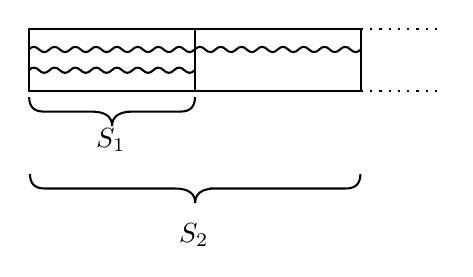
\begin{tikzpicture}[x=0.75pt,y=0.75pt,yscale=-1,xscale=1]
		%uncomment if require: \path (0,300); %set diagram left start at 0, and has height of 300

		%Shape: Brace [id:dp6450376307720747] 
		\draw   (150.22,152.93) .. controls (150.22,157.6) and (152.55,159.93) .. (157.22,159.93) -- (180.17,159.93) .. controls (186.84,159.93) and (190.17,162.26) .. (190.17,166.93) .. controls (190.17,162.26) and (193.5,159.93) .. (200.17,159.93)(197.17,159.93) -- (223.11,159.93) .. controls (227.78,159.93) and (230.11,157.6) .. (230.11,152.93) ;
		%Shape: Brace [id:dp6867457932235534] 
		\draw   (150.62,189.98) .. controls (150.62,194.65) and (152.95,196.98) .. (157.62,196.98) -- (220.21,196.98) .. controls (226.88,196.98) and (230.21,199.31) .. (230.21,203.98) .. controls (230.21,199.31) and (233.54,196.98) .. (240.21,196.98)(237.21,196.98) -- (302.8,196.98) .. controls (307.47,196.98) and (309.8,194.65) .. (309.8,189.98) ;
		%Shape: Rectangle [id:dp04043578965235095] 
		\draw   (150,120) -- (310,120) -- (310,150) -- (150,150) -- cycle ;
		%Straight Lines [id:da7948124479327557] 
		\draw    (230,120) -- (230,150) ;
		%Straight Lines [id:da6507675221013395] 
		\draw    (150,140) .. controls (151.67,138.33) and (153.33,138.33) .. (155,140) .. controls (156.67,141.67) and (158.33,141.67) .. (160,140) .. controls (161.67,138.33) and (163.33,138.33) .. (165,140) .. controls (166.67,141.67) and (168.33,141.67) .. (170,140) .. controls (171.67,138.33) and (173.33,138.33) .. (175,140) .. controls (176.67,141.67) and (178.33,141.67) .. (180,140) .. controls (181.67,138.33) and (183.33,138.33) .. (185,140) .. controls (186.67,141.67) and (188.33,141.67) .. (190,140) .. controls (191.67,138.33) and (193.33,138.33) .. (195,140) .. controls (196.67,141.67) and (198.33,141.67) .. (200,140) .. controls (201.67,138.33) and (203.33,138.33) .. (205,140) .. controls (206.67,141.67) and (208.33,141.67) .. (210,140) .. controls (211.67,138.33) and (213.33,138.33) .. (215,140) .. controls (216.67,141.67) and (218.33,141.67) .. (220,140) .. controls (221.67,138.33) and (223.33,138.33) .. (225,140) .. controls (226.67,141.67) and (228.33,141.67) .. (230,140) -- (230,140) ;
		%Straight Lines [id:da816948397241291] 
		\draw    (150,130) .. controls (151.67,128.33) and (153.33,128.33) .. (155,130) .. controls (156.67,131.67) and (158.33,131.67) .. (160,130) .. controls (161.67,128.33) and (163.33,128.33) .. (165,130) .. controls (166.67,131.67) and (168.33,131.67) .. (170,130) .. controls (171.67,128.33) and (173.33,128.33) .. (175,130) .. controls (176.67,131.67) and (178.33,131.67) .. (180,130) .. controls (181.67,128.33) and (183.33,128.33) .. (185,130) .. controls (186.67,131.67) and (188.33,131.67) .. (190,130) .. controls (191.67,128.33) and (193.33,128.33) .. (195,130) .. controls (196.67,131.67) and (198.33,131.67) .. (200,130) .. controls (201.67,128.33) and (203.33,128.33) .. (205,130) .. controls (206.67,131.67) and (208.33,131.67) .. (210,130) .. controls (211.67,128.33) and (213.33,128.33) .. (215,130) .. controls (216.67,131.67) and (218.33,131.67) .. (220,130) .. controls (221.67,128.33) and (223.33,128.33) .. (225,130) .. controls (226.67,131.67) and (228.33,131.67) .. (230,130) .. controls (231.67,128.33) and (233.33,128.33) .. (235,130) .. controls (236.67,131.67) and (238.33,131.67) .. (240,130) .. controls (241.67,128.33) and (243.33,128.33) .. (245,130) .. controls (246.67,131.67) and (248.33,131.67) .. (250,130) .. controls (251.67,128.33) and (253.33,128.33) .. (255,130) .. controls (256.67,131.67) and (258.33,131.67) .. (260,130) .. controls (261.67,128.33) and (263.33,128.33) .. (265,130) .. controls (266.67,131.67) and (268.33,131.67) .. (270,130) .. controls (271.67,128.33) and (273.33,128.33) .. (275,130) .. controls (276.67,131.67) and (278.33,131.67) .. (280,130) .. controls (281.67,128.33) and (283.33,128.33) .. (285,130) .. controls (286.67,131.67) and (288.33,131.67) .. (290,130) .. controls (291.67,128.33) and (293.33,128.33) .. (295,130) .. controls (296.67,131.67) and (298.33,131.67) .. (300,130) .. controls (301.67,128.33) and (303.33,128.33) .. (305,130) .. controls (306.67,131.67) and (308.33,131.67) .. (310,130) -- (310,130) ;
		%Straight Lines [id:da005001855200690519] 
		\draw  [dash pattern={on 0.84pt off 2.51pt}]  (310,120) -- (350,120) ;
		%Straight Lines [id:da8158288414744241] 
		\draw  [dash pattern={on 0.84pt off 2.51pt}]  (310,150) -- (350,150) ;

		% Text Node
		\draw (181,166.4) node [anchor=north west][inner sep=0.75pt]    {$S_{1}$};
		% Text Node
		\draw (221,212.4) node [anchor=north west][inner sep=0.75pt]    {$S_{2}$};
	\end{tikzpicture}
	\caption{$S_2$ è il numero di $1$ presenti in $\mathbf{b}$ `sotto' la traccia più lunga, mentre $S_1$
		è il numero di $1$ sotto quella più corta. Va notato che $S_0 = 0$ benché non sia
		mostrato nella figura.}
	\label{fig:superblock_i}
\end{figure}
Per ogni blocco $l$ afferente al superblocco $i$ si definisce
$$
	B_l = \mathbf{rank}(l[0]) - S_i
$$
come rappresentato nella \cref{fig:block_i}.
\begin{figure}
	\centering



	\tikzset{every picture/.style={line width=0.75pt}} %set default line width to 0.75pt        

	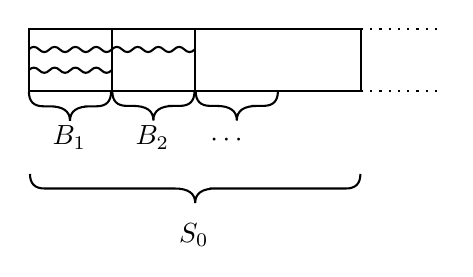
\begin{tikzpicture}[x=0.75pt,y=0.75pt,yscale=-1,xscale=1]
		%uncomment if require: \path (0,300); %set diagram left start at 0, and has height of 300

		%Shape: Brace [id:dp6867457932235534] 
		\draw   (150.62,189.98) .. controls (150.62,194.65) and (152.95,196.98) .. (157.62,196.98) -- (220.21,196.98) .. controls (226.88,196.98) and (230.21,199.31) .. (230.21,203.98) .. controls (230.21,199.31) and (233.54,196.98) .. (240.21,196.98)(237.21,196.98) -- (302.8,196.98) .. controls (307.47,196.98) and (309.8,194.65) .. (309.8,189.98) ;
		%Shape: Rectangle [id:dp04043578965235095] 
		\draw   (150,120) -- (310,120) -- (310,150) -- (150,150) -- cycle ;
		%Straight Lines [id:da005001855200690519] 
		\draw  [dash pattern={on 0.84pt off 2.51pt}]  (310,120) -- (350,120) ;
		%Straight Lines [id:da8158288414744241] 
		\draw  [dash pattern={on 0.84pt off 2.51pt}]  (310,150) -- (350,150) ;
		%Shape: Brace [id:dp13835137879055492] 
		\draw   (150.09,150.38) .. controls (150.09,155.05) and (152.42,157.38) .. (157.09,157.38) -- (159.88,157.38) .. controls (166.55,157.38) and (169.88,159.71) .. (169.88,164.38) .. controls (169.88,159.71) and (173.21,157.38) .. (179.88,157.38)(176.88,157.38) -- (182.67,157.38) .. controls (187.34,157.38) and (189.67,155.05) .. (189.67,150.38) ;
		%Shape: Brace [id:dp46357313811514655] 
		\draw   (190.28,150.18) .. controls (190.28,154.85) and (192.61,157.18) .. (197.28,157.18) -- (200.07,157.18) .. controls (206.74,157.18) and (210.07,159.51) .. (210.07,164.18) .. controls (210.07,159.51) and (213.4,157.18) .. (220.07,157.18)(217.07,157.18) -- (222.86,157.18) .. controls (227.53,157.18) and (229.86,154.85) .. (229.86,150.18) ;
		%Shape: Brace [id:dp8791020491294269] 
		\draw   (230.47,150.18) .. controls (230.47,154.85) and (232.8,157.18) .. (237.47,157.18) -- (240.26,157.18) .. controls (246.93,157.18) and (250.26,159.51) .. (250.26,164.18) .. controls (250.26,159.51) and (253.59,157.18) .. (260.26,157.18)(257.26,157.18) -- (263.05,157.18) .. controls (267.72,157.18) and (270.05,154.85) .. (270.05,150.18) ;
		%Straight Lines [id:da2991531768387089] 
		\draw    (190,120) -- (190,150) ;
		%Straight Lines [id:da7604970738017156] 
		\draw    (230,120) -- (230,150) ;
		%Straight Lines [id:da9790584425339227] 
		\draw    (150,140) .. controls (151.67,138.33) and (153.33,138.33) .. (155,140) .. controls (156.67,141.67) and (158.33,141.67) .. (160,140) .. controls (161.67,138.33) and (163.33,138.33) .. (165,140) .. controls (166.67,141.67) and (168.33,141.67) .. (170,140) .. controls (171.67,138.33) and (173.33,138.33) .. (175,140) .. controls (176.67,141.67) and (178.33,141.67) .. (180,140) .. controls (181.67,138.33) and (183.33,138.33) .. (185,140) .. controls (186.67,141.67) and (188.33,141.67) .. (190,140) -- (190,140) ;
		%Straight Lines [id:da7640613174865398] 
		\draw    (150,130) .. controls (151.67,128.33) and (153.33,128.33) .. (155,130) .. controls (156.67,131.67) and (158.33,131.67) .. (160,130) .. controls (161.67,128.33) and (163.33,128.33) .. (165,130) .. controls (166.67,131.67) and (168.33,131.67) .. (170,130) .. controls (171.67,128.33) and (173.33,128.33) .. (175,130) .. controls (176.67,131.67) and (178.33,131.67) .. (180,130) .. controls (181.67,128.33) and (183.33,128.33) .. (185,130) .. controls (186.67,131.67) and (188.33,131.67) .. (190,130) .. controls (191.67,128.33) and (193.33,128.33) .. (195,130) .. controls (196.67,131.67) and (198.33,131.67) .. (200,130) .. controls (201.67,128.33) and (203.33,128.33) .. (205,130) .. controls (206.67,131.67) and (208.33,131.67) .. (210,130) .. controls (211.67,128.33) and (213.33,128.33) .. (215,130) .. controls (216.67,131.67) and (218.33,131.67) .. (220,130) .. controls (221.67,128.33) and (223.33,128.33) .. (225,130) .. controls (226.67,131.67) and (228.33,131.67) .. (230,130) -- (230,130) ;

		% Text Node
		\draw (221,212.4) node [anchor=north west][inner sep=0.75pt]    {$S_{0}$};
		% Text Node
		\draw (160,165.4) node [anchor=north west][inner sep=0.75pt]    {$B_{1}$};
		% Text Node
		\draw (200,165.4) node [anchor=north west][inner sep=0.75pt]    {$B_{2}$};
		% Text Node
		\draw (236,169.4) node [anchor=north west][inner sep=0.75pt]    {$\cdots $};
	\end{tikzpicture}
	\caption{$B_2$ è il numero di $1$ presenti in $\mathbf{b}$ `sotto' la traccia più lunga, mentre $B_1$
		è il numero di $1$ sotto quella più corta. Va notato che $B_0$, in questo frangente, è $0$,
		poiché $S_0$ è il primo superblocco di $\mathbf{b}$.}
	\label{fig:block_i}
\end{figure}

\noindent
Quindi, gli $S_i$ sono tanti quanti sono i superblocchi, ossia $\frac{n}{log_2(n)^2}$ e occupano spazio
$$
	\frac{n}{\log_2(n)^2} \underbrace{\log_2(n)}_{\text{spazio di un } S_I} = \frac{n}{\log_2(n)} = o(n) \text{ bit}
$$
mentre i $B_l$ sono tanti quanti sono i blocchi, ossia $\frac{n}{\frac{1}{2}\log_2(n)}$ e occupano spazio
$$
	\frac{n}{\frac{1}{2}\log_2(n)} \underbrace{\log_2(\log_2(n)^2)}_{\text{al massimo}} =
	\frac{2n}{\log_2(n)} 2 \log_2(\log_2(n)) = o(n) \text{ bit}
$$
Se si vuole conoscere il rango di uno specifico bit in un blocco bisogna
recuperare $S_i$ e $B_i$ e calcolare il quale sia effettivamente il rango, che
è stato memorizzato in una tabella $Tab$ utilizzando il four-russians trick
enumerando i possibili $\sqrt(n)$ blocchi e memorizzando il rango di ogni
bit del blocco. Complessivamente, quindi, tutte le tabelle necessarie occupano
$D_n = o(n)$ bit.

\begin{figure}[!h]
	\centering
	\tikzset{every picture/.style={line width=0.75pt}} %set default line width to 0.75pt        

	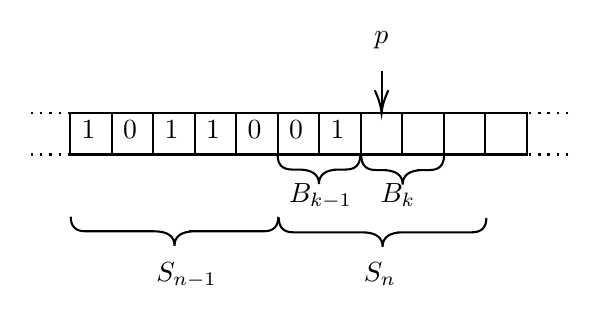
\begin{tikzpicture}[x=0.75pt,y=0.75pt,yscale=-1,xscale=1]
		%uncomment if require: \path (0,300); %set diagram left start at 0, and has height of 300

		%Shape: Rectangle [id:dp07152433688787241] 
		\draw   (100,100) -- (320,100) -- (320,120) -- (100,120) -- cycle ;
		%Straight Lines [id:da2936448051112307] 
		\draw    (120,100) -- (120,120) ;
		%Straight Lines [id:da027036583121563318] 
		\draw    (140,100) -- (140,120) ;
		%Straight Lines [id:da7810766858201694] 
		\draw    (160,100) -- (160,120) ;
		%Straight Lines [id:da5001340947135379] 
		\draw    (180,100) -- (180,120) ;
		%Straight Lines [id:da3843632481846373] 
		\draw    (200,100) -- (200,120) ;
		%Straight Lines [id:da03824030730667982] 
		\draw    (220,100) -- (220,120) ;
		%Straight Lines [id:da15646574434271243] 
		\draw    (240,100) -- (240,120) ;
		%Straight Lines [id:da846809534956415] 
		\draw    (260,100) -- (260,120) ;
		%Straight Lines [id:da4897590587430042] 
		\draw    (280,100) -- (280,120) ;
		%Straight Lines [id:da4069787777904943] 
		\draw    (300,100) -- (300,120) ;
		%Straight Lines [id:da05219000701716625] 
		\draw    (250,80) -- (250,98) ;
		\draw [shift={(250,100)}, rotate = 270] [color={rgb, 255:red, 0; green, 0; blue, 0 }  ][line width=0.75]    (10.93,-3.29) .. controls (6.95,-1.4) and (3.31,-0.3) .. (0,0) .. controls (3.31,0.3) and (6.95,1.4) .. (10.93,3.29)   ;
		%Shape: Brace [id:dp37474184805141453] 
		\draw   (100.25,150) .. controls (100.25,154.67) and (102.58,157) .. (107.25,157) -- (140.25,157) .. controls (146.92,157) and (150.25,159.33) .. (150.25,164) .. controls (150.25,159.33) and (153.58,157) .. (160.25,157)(157.25,157) -- (193.25,157) .. controls (197.92,157) and (200.25,154.67) .. (200.25,150) ;
		%Shape: Brace [id:dp9417201733674553] 
		\draw   (200.5,150.5) .. controls (200.5,155.17) and (202.83,157.5) .. (207.5,157.5) -- (240.5,157.5) .. controls (247.17,157.5) and (250.5,159.83) .. (250.5,164.5) .. controls (250.5,159.83) and (253.83,157.5) .. (260.5,157.5)(257.5,157.5) -- (293.5,157.5) .. controls (298.17,157.5) and (300.5,155.17) .. (300.5,150.5) ;
		%Straight Lines [id:da1555835238266523] 
		\draw  [dash pattern={on 0.84pt off 2.51pt}]  (100,100) -- (80,100) ;
		%Straight Lines [id:da0928939361477803] 
		\draw  [dash pattern={on 0.84pt off 2.51pt}]  (100,120) -- (80,120) ;
		%Straight Lines [id:da19581834915337515] 
		\draw  [dash pattern={on 0.84pt off 2.51pt}]  (340,120) -- (320,120) ;
		%Straight Lines [id:da4107689408293117] 
		\draw  [dash pattern={on 0.84pt off 2.51pt}]  (340,100) -- (320,100) ;
		%Shape: Brace [id:dp9863486277907854] 
		\draw   (240.25,120.5) .. controls (240.25,125.17) and (242.58,127.5) .. (247.25,127.5) -- (250.17,127.5) .. controls (256.84,127.5) and (260.17,129.83) .. (260.17,134.5) .. controls (260.17,129.83) and (263.5,127.5) .. (270.17,127.5)(267.17,127.5) -- (273.08,127.5) .. controls (277.75,127.5) and (280.08,125.17) .. (280.08,120.5) ;
		%Shape: Brace [id:dp8556326349440747] 
		\draw   (199.92,120.25) .. controls (199.92,124.92) and (202.25,127.25) .. (206.92,127.25) -- (209.83,127.25) .. controls (216.5,127.25) and (219.83,129.58) .. (219.83,134.25) .. controls (219.83,129.58) and (223.16,127.25) .. (229.83,127.25)(226.83,127.25) -- (232.75,127.25) .. controls (237.42,127.25) and (239.75,124.92) .. (239.75,120.25) ;

		% Text Node
		\draw (245,59.4) node [anchor=north west][inner sep=0.75pt]    {$p$};
		% Text Node
		\draw (104,102.4) node [anchor=north west][inner sep=0.75pt]    {$1$};
		% Text Node
		\draw (124,102.4) node [anchor=north west][inner sep=0.75pt]    {$0$};
		% Text Node
		\draw (144,102.4) node [anchor=north west][inner sep=0.75pt]    {$1$};
		% Text Node
		\draw (224,102.4) node [anchor=north west][inner sep=0.75pt]    {$1$};
		% Text Node
		\draw (164,102.4) node [anchor=north west][inner sep=0.75pt]    {$1$};
		% Text Node
		\draw (204,102.4) node [anchor=north west][inner sep=0.75pt]    {$0$};
		% Text Node
		\draw (240,170.4) node [anchor=north west][inner sep=0.75pt]    {$S_{n}$};
		% Text Node
		\draw (140,170.4) node [anchor=north west][inner sep=0.75pt]    {$S_{n-1}$};
		% Text Node
		\draw (248,132.4) node [anchor=north west][inner sep=0.75pt]    {$B_{k}$};
		% Text Node
		\draw (204,132.4) node [anchor=north west][inner sep=0.75pt]    {$B_{k-1}$};
		% Text Node
		\draw (184,102.4) node [anchor=north west][inner sep=0.75pt]    {$0$};
	\end{tikzpicture}
	\caption{Calcolo di $\mathbf{rank_b}(p)$.}
	\label{fig:example_rank_p}
\end{figure}

Quanto tempo impiega un'implementazione basata su queste strutture per
calcolare il rango di una posizione $p$? Per sapere quanti $1$ ci sono
prima della posizione $p$, bisogna innanzitutto calcolare il superblocco
di appartenenza di $p$, che è il superblocco numero $\frac{p}{\log_2(n)^2}$.
Vogliamo sapere quanti $1$ ci sono prima di quel superblocco - valore che abbiamo
memorizzato nei $S_i$. A questo punto, è necessario calcolare il numero di $1$
dall'inizio del superblocco all'inizio del blocco al quale appartiene $p$, valore salvato
in $B_i$. Rimane, quindi, da capire quanti $1$ ci sono dall'inizio del blocco al
quale appartiene $p$ fino alla posizione $p$ stessa. Per questo si può
utilizzare la tabella $Tab$ del four-russians trick:

$$
	\mathbf{rank}_{\mathbf{b}}(p) = S_{\frac{p}{\log_2(n)^2}} + B_{\frac{p}{\frac{1}{2}\log_2(n)}}
	+ Tab[t, p \mod \frac{1}{2}\log_2(n)]
$$
dove $t$ è il tipo blocco a cui $p$ appartiene secondo l'enumerazione dei blocchi di
$Tab$, calcolabile data la posizione d'inizio del blocco di $p$
$$
	x = \lfloor \frac{p}{\frac{1}{2}\log_2(n)}\rfloor (\frac{1}{2}\log_2(n))
$$
accedendo il vettore $\mathbf{b}$ e leggendo i valori del blocco\footnote{
	In termini pratici, come avviene questo accesso? Se avviene leggendo,
	uno per uno, tutti i valori del blocco al quale appartiene $p$ per poi
	accedere alla tabella $Tab$, non ha più senso leggere i valori da
	$\mathbf{b}[x]$ fino a $\mathbf{b}[p-1]$ contando gli $1$ visti?
}:
$$
	t = \mathbf{b}[x, x +1, \cdots, x + \frac{1}{2} \log_2(n) -1 ]
$$
Il calcolo del rank avviene quindi in tempo lineare,
poiché si tratta di accedere a $3$ tabelle e la struttura quindi
occupa lo spazio di $n + o(n)$ bit, poiché è necessario mantenere $b$ e
risponde alle query in tempo $O(1)$. Rispetto alla nostra classificazione,
questa struttura è \textbf{succinta} e ha la stessa efficienza della struttura naïve.

\subsection{Struttura di Clarke per la selezione}
La struttura di Clarke per la selezione è succinta teoricamente, ma in pratica
è raramente utilizzata come descritta perché la sua implementazione è molto
complessa.
L'obiettivo è, dato un vettore $\mathbf{b}$ di valori binari fissato, calcolare
la funzione di selezione
$$
	\mathbf{select_b}(k) = \text{ posizione del } k-\text{esimo } 1
$$
La struttura di Clarke utilizza dei \textit{livelli}, simili a quelli utilizzati
dalla struttura di Jacobson.

\subsubsection{Primo livello}
Il primo livello della struttura di Clarke è un insieme
di valori che rappresentano le posizioni degli $1$ di ordinalità multipla di
$\log_2(n) \cdot \log_2(\log_2(n))$, ossia
$$
	P_i =  \mathbf{select_b}(i \cdot \log_2(n) \cdot \log_2(\log_2(n)))
$$
ossia la posizione del $(i \cdot \log_2(n) \cdot \log_2(\log_2(n)))$-esimo $1$.

\paragraph{Memoria}
La grandezza di questa famiglia, ossia il numero di $P_i$, dipende dal
numero di $i$ che ci sono in $\mathbf{b}$, ma nel caso peggiore, il vettore
è composto unicamente da $1$ e vi saranno $\frac{n}{\log_2(n) \cdot \log_2(\log_2(n))}$ membri.
Ad ognuno di essi va associato un elemento, il quale richiede $\log_2(n)$ bit;
in totale, questo livello occupa
$$
	\frac{n}{\log_2(n) \cdot \log_2(\log_2(n))} \cdot \log_2(n) = o(n) \text{ bit}
$$

\subsubsection{Secondo livello}
Per le posizioni che non sono multiple di $\log_2(n) \cdot \log_2(\log_2(n))$ si utilizza
un secondo livello, che è costruito differentemente in base ad un indice calcolato
per ogni $P_i$:

$$
	\forall i ~ r_i = P_{i + 1} - P_i
$$
che rappresenta la distanza fra l'$(i \cdot \log_2(n) \cdot \log_2(\log_2(n)))$-esimo $1$
e il $((i+1) \cdot \log_2(n) \cdot \log_2(\log_2(n)))$-esimo. Questo
valore, $r_i$, sarà esattamente uguale a $\log_2(n) \cdot \log_2(\log_2(n))$ se e solo se
tra $P_{i}$ e $P_{i+1}$ ci sono unicamente $1$, e sarà maggiore se invece le
due posizioni sono più lontane.
% @TODO: serve un esempio, non si capisce bene. 
I due casi che si considerano dipendono dal valore di $r_i$.

\paragraph{Caso sparso}
Se $r_i \geq (\log_2(n) \cdot \log_2(\log_2(n)))^2$, significa che in $\mathbf{b}$ ci
sono molti $0$ tra gli $1$ contenuti nelle posizioni tra $P_{i}$ e $P_{i+1}$; in questo caso
definiamo $S_i$ come la lista esplicita delle posizioni di tutti gli $1$
in $\mathbf{b}$ tra le due posizioni rappresentate come differenza tra $P_i$.

In questo caso, gli $S_i$ costruiti sono esattamente $\log_2(n)\cdot \log_2(\log_2(n))$,
in quanto stiamo contando gli $1$ in $\mathbf{b}$ tra il $(i \cdot \log_2(n) \cdot \log_2(\log_2(n))$-esimo
$1$ e il $((i+1) \cdot \log_2(n) \cdot \log_2(\log_2(n))$-esimo $1$, e ad ognuno
di essi si associa un numero che in grandezza è minore o uguale a
$\log_2(r_i)$, concludendo che per memorizzare un $S_i$ sono necessari
\begin{align*}
	\log_2(n)\cdot \log_2(\log_2(n)) \cdot \log_2(r_i) & = \frac{(\log_2(n)\cdot \log_2(\log_2(n)))^2}{\log_2(n)\cdot \log_2(\log_2(n))} \cdot \log_2(r_i) \\
	                                                   & \leq \frac{r_i}{\log_2(n)\cdot \log_2(\log_2(n))} \cdot \log_2(r_i)                               \\
	                                                   & \leq \frac{r_i}{\log_2(n)\cdot \log_2(\log_2(n))} \cdot \log_2(n)                                 \\
	                                                   & \leq \frac{r_i}{\log_2(\log_2(n))}                                                                \\
	                                                   & \leq \frac{n}{\log_2(\log_2(n))}   = o(n) \text{ bit}
\end{align*}

\paragraph{Caso denso}
Se $r_i \le (\log_2(n) \cdot \log_2(\log_2(n)))^2$, si memorizzano gli $1$
multipli di $\log_2(r_i)\log_2(\log_2(n))$, ossia partendo dalla posizione $P_i$ si salvano le
posizioni degli $j \cdot \log_2(r_i)\log_2(\log_2(n))$-esimi $1$ come differenze da $P_i$, ossia
$$
	S^i_j = \mathbf{select_b}(j \cdot \log_2(r_i)\log_2(\log_2(n))) - P_i
$$

In questo caso, gli $1$ memorizzati sono $\frac{\log_2(n)\cdot \log_2(\log_2(n))}{\log_2(r_i)\cdot \log_2(\log_2(n))}$.
Ad ognuno di questi si associa un valore in grandezza $\log_2(r_i)$, quindi lo spazio utilizzato
per memorizzare tutti i valori $S^i_j$ sono
$$
	\frac{\log_2(n)\cdot \log_2(\log_2(n))}{\log_2(r_i)\cdot \log_2(\log_2(n))} \log_2(r_i) =
	\frac{\log_2(n)\cdot \log_2(\log_2(n))}{\log_2(\log_2(n))} \leq \frac{r_i}{\log_2(\log_2(n))}
	\leq \frac{n}{\log_2(\log_2(n))} = o(n) \text{ bit}
$$


\subsubsection{Terzo livello}
Se nel secondo livello ci si trova nel caso denso, si utilizza un terzo livello.
Questo livello viene utilizzato esclusivamente per gli $1$ le cui posizioni non sono state
salvate nel secondo livello nel caso denso; pertanto, l'assunto è che
$$
	r_i < (\log_2(n) \log_2(\log_2(n)))^2
$$
Per ognuna di queste posizioni calcoliamo la differenza tra $S^i_j$:
$$
	\forall j ~~ \bar{r}^i_j = S^i_{j+1} - S^i_j
$$
Come nel caso precedente, abbiamo due possibilità in base al valore di $\bar{r}^i_j$, il quale
gode comunque della proprietà
$$
	\forall i, j ~~  \bar{r}^i_j \geq \log_2(r_i) \log_2(\log_2(n))
$$
\paragraph{Caso sparso}
Nel caso in cui $\bar{r}^i_j \geq \log_2(\bar{r}^i_j) \log_2(r_i) \log_2(\log_2(n))^2$,
si memorizzano esplicitamente tutte le posizioni degli $1$ tra $S^i_j$ e $S^i_{j+1}$
con dei valori $T^i_{j,k}$ come differenze tra $S^i_j$. In questo caso,
il consumo di memoria è
$$
	(\log_2(r_i)\cdot \log_2(\log_2(n)) \cdot \log_2(\bar{r}^i_j) \leq
	\frac{\log_2(r_i) \cdot \log_2(\log_2(n))^2 \log_2(\bar{r}^i_j)}{\log_2(\log_2(n))}
	\leq \frac{\bar{r}^i_j}{\log_2(\log_2(n))} = o(n) \text{ bit}
$$
\paragraph{Caso denso}
Nel caso in cui $\bar{r}^i_j \le \log_2(\bar{r}^i_j) \log_2(r_i) \log_2(\log_2(n))^2$,
significa che ci sono pochi $0$ tra $S^i_j$ e $S^i_{j+1}$ e
si utilizza il four-russians trick. Inizialmente osserviamo quanto segue.
\begin{oss}
	\begin{align*}
		\log_2(\bar{r}^i_j) \leq \log_2(r_i) & \leq \log_2(\log_2(n)\cdot \log_2(\log_2(n)))^2     \\
		                                     & = 2 \log_2(\log_2(n)) + 2 \log_2(\log_2(\log_2(n))) \\
		                                     & \leq 4 \log_2(\log_2(n))
	\end{align*}
\end{oss}
\begin{oss}
	$$
		\bar{r}^i_j < \log_2(\bar{r}^i_j) \cdot \log_2(r_i) \cdot (\log_2(\log_2(n))^2
		\leq 16(\log_2\log_2(n))^4
	$$
\end{oss}
Lo spazio necessario per utilizzare il four-russians trick è quanto segue.
Servono $2^{\bar{r}^i_j}$ enumerazioni di `sottovettori',
ossia la dimensione tra $S^i_j$ e $S^i_{j+1}$,
che è la parte che va memorizzata esplicitamente; per ognuna di queste
enumerazioni è necessario salvare la posizione di $\bar{r}^i_j$ $1$ utilizzando
memoria al massimo $\log_2(\bar{r}^i_j)$:
\begin{align*}
	2^{\bar{r}^i_j} \cdot \bar{r}^i_j \cdot \log_2(\bar{r}^i_j) & \leq
	2^{16(\log_2\log_2(n))^4} \cdot 16(\log_2\log_2(n))^4 \cdot \log_2(16(\log_2\log_2(n))^4)                                  \\
	                                                            & = 16(\log_2\log_2(n))^8 \log_2(16(\log_2\log_2(n))^4) = o(n)
\end{align*}


\subsubsection{Complessità totale in spazio}
In totale, per memorizzare $\mathbf{b}$ e i possibili tre livelli di struttura,
sono necessari $o(n)$ bit per il primo livello e, in base a come è fatto il secondo livello
$$
	\sum^{\frac{n}{\log_2(n)\cdot \log_2(\log_2(n))}} \frac{P_{i+1} - P_i}{\log_2(\log_2(n)}
	= \frac{P_n - P_0}{\log_2(\log_2(n))}
	\leq \frac{n}{\log_2(\log_2(n))} = o(n) \text{ bit}
$$
più $o(n)$ bit per il terzo livello. Quindi, la struttura di Clarke occupa
spazio $n + o(n)$ e ha tempo di accesso costante, pertanto è
una struttura \textbf{succinta}.

\begin{figure}
	\centering
	\tikzset{every picture/.style={line width=0.75pt}} %set default line width to 0.75pt        

	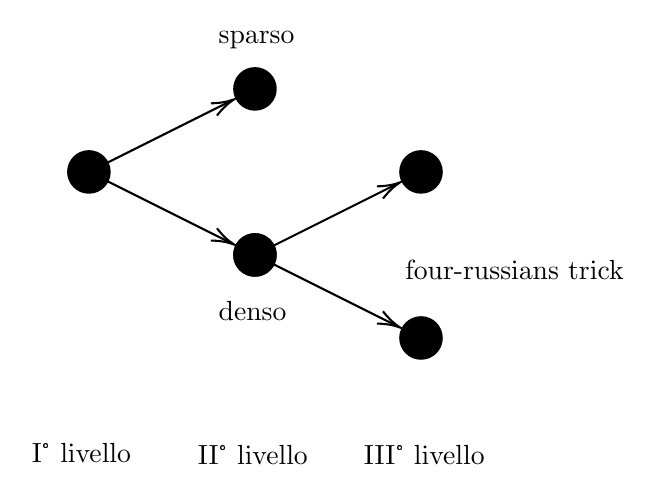
\begin{tikzpicture}[x=0.75pt,y=0.75pt,yscale=-1,xscale=1]
		%uncomment if require: \path (0,300); %set diagram left start at 0, and has height of 300

		%Shape: Circle [id:dp9914836432536758] 
		\draw  [fill={rgb, 255:red, 0; green, 0; blue, 0 }  ,fill opacity=1 ] (70,101) .. controls (70,95.48) and (74.48,91) .. (80,91) .. controls (85.52,91) and (90,95.48) .. (90,101) .. controls (90,106.52) and (85.52,111) .. (80,111) .. controls (74.48,111) and (70,106.52) .. (70,101) -- cycle ;
		%Shape: Circle [id:dp09703813871749656] 
		\draw  [fill={rgb, 255:red, 0; green, 0; blue, 0 }  ,fill opacity=1 ] (150,61) .. controls (150,55.48) and (154.48,51) .. (160,51) .. controls (165.52,51) and (170,55.48) .. (170,61) .. controls (170,66.52) and (165.52,71) .. (160,71) .. controls (154.48,71) and (150,66.52) .. (150,61) -- cycle ;
		%Straight Lines [id:da8346853138498954] 
		\draw    (80,101) -- (148.21,66.89) ;
		\draw [shift={(150,66)}, rotate = 153.43] [color={rgb, 255:red, 0; green, 0; blue, 0 }  ][line width=0.75]    (10.93,-3.29) .. controls (6.95,-1.4) and (3.31,-0.3) .. (0,0) .. controls (3.31,0.3) and (6.95,1.4) .. (10.93,3.29)   ;
		%Shape: Circle [id:dp4565729376211175] 
		\draw  [fill={rgb, 255:red, 0; green, 0; blue, 0 }  ,fill opacity=1 ] (150,141) .. controls (150,146.52) and (154.48,151) .. (160,151) .. controls (165.52,151) and (170,146.52) .. (170,141) .. controls (170,135.48) and (165.52,131) .. (160,131) .. controls (154.48,131) and (150,135.48) .. (150,141) -- cycle ;
		%Straight Lines [id:da8127484960209145] 
		\draw    (80,101) -- (148.21,135.11) ;
		\draw [shift={(150,136)}, rotate = 206.57] [color={rgb, 255:red, 0; green, 0; blue, 0 }  ][line width=0.75]    (10.93,-3.29) .. controls (6.95,-1.4) and (3.31,-0.3) .. (0,0) .. controls (3.31,0.3) and (6.95,1.4) .. (10.93,3.29)   ;
		%Shape: Circle [id:dp546530222511162] 
		\draw  [fill={rgb, 255:red, 0; green, 0; blue, 0 }  ,fill opacity=1 ] (150,141) .. controls (150,135.48) and (154.48,131) .. (160,131) .. controls (165.52,131) and (170,135.48) .. (170,141) .. controls (170,146.52) and (165.52,151) .. (160,151) .. controls (154.48,151) and (150,146.52) .. (150,141) -- cycle ;
		%Shape: Circle [id:dp1691093585413369] 
		\draw  [fill={rgb, 255:red, 0; green, 0; blue, 0 }  ,fill opacity=1 ] (230,101) .. controls (230,95.48) and (234.48,91) .. (240,91) .. controls (245.52,91) and (250,95.48) .. (250,101) .. controls (250,106.52) and (245.52,111) .. (240,111) .. controls (234.48,111) and (230,106.52) .. (230,101) -- cycle ;
		%Straight Lines [id:da17118221437478087] 
		\draw    (160,141) -- (228.21,106.89) ;
		\draw [shift={(230,106)}, rotate = 153.43] [color={rgb, 255:red, 0; green, 0; blue, 0 }  ][line width=0.75]    (10.93,-3.29) .. controls (6.95,-1.4) and (3.31,-0.3) .. (0,0) .. controls (3.31,0.3) and (6.95,1.4) .. (10.93,3.29)   ;
		%Shape: Circle [id:dp8870903616648642] 
		\draw  [fill={rgb, 255:red, 0; green, 0; blue, 0 }  ,fill opacity=1 ] (230,181) .. controls (230,186.52) and (234.48,191) .. (240,191) .. controls (245.52,191) and (250,186.52) .. (250,181) .. controls (250,175.48) and (245.52,171) .. (240,171) .. controls (234.48,171) and (230,175.48) .. (230,181) -- cycle ;
		%Straight Lines [id:da2110125336208042] 
		\draw    (160,141) -- (228.21,175.11) ;
		\draw [shift={(230,176)}, rotate = 206.57] [color={rgb, 255:red, 0; green, 0; blue, 0 }  ][line width=0.75]    (10.93,-3.29) .. controls (6.95,-1.4) and (3.31,-0.3) .. (0,0) .. controls (3.31,0.3) and (6.95,1.4) .. (10.93,3.29)   ;

		% Text Node
		\draw (51,230) node [anchor=north west][inner sep=0.75pt]   [align=left] {I° livello};
		% Text Node
		\draw (131,231) node [anchor=north west][inner sep=0.75pt]   [align=left] {II° livello};
		% Text Node
		\draw (211,231) node [anchor=north west][inner sep=0.75pt]   [align=left] {III° livello};
		% Text Node
		\draw (141,162) node [anchor=north west][inner sep=0.75pt]   [align=left] {denso};
		% Text Node
		\draw (141,32) node [anchor=north west][inner sep=0.75pt]   [align=left] {sparso};
		% Text Node
		\draw (231,142) node [anchor=north west][inner sep=0.75pt]   [align=left] {four-russians trick};
	\end{tikzpicture}
	\caption{Struttura di Clarke per la selezione.}
\end{figure}



% lezione 19 - 01-12-2021
\section{Struttura per alberi binari}
Gli \textit{alberi} possono essere visti in due modi: per i
matematici, essi sono dei grafi connessi aciclici mentre per gli
informatici sono una \textit{struttura dati} radicata che ha una
\textit{radice}. In particolare, un albero \textit{binario} è un
albero tale per cui ogni nodo ha al più due figli; formalmente,
si definiscono induttivamente: l'albero con un solo nodo (che è anche
la radice), denotato $\emptyset$, è un albero binario;
se $T_1$ e $T_2$ sono due alberi binari,
allora anche l'albero radicato in un nuovo nodo che ha come figli
$T_1$ e $T_2$, denotato $(T_1, T_2)$ è un albero binario. In questa definizione,
ogni nodo ha o $0$ o $2$ figli. I nodi che non hanno figli
sono chiamati \textbf{nodi esterni} o \textbf{foglie}, mentre gli altri sono
chiamati \textbf{nodi interni}.


\begin{figure}[!hb]
	\begin{subfigure}{0.45\textwidth}
		\begin{center}
			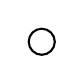
\begin{tikzpicture}
				\node [circle, draw]{};
			\end{tikzpicture}
		\end{center}
		\caption{L'albero binario $\emptyset$.}
	\end{subfigure}
	\begin{subfigure}{0.45\textwidth}
		\begin{center}
			\begin{tikzpicture}
				\node [circle,draw]{}
				child {node [isosceles triangle,draw,shape border rotate=90] {$T_1$}}
				child {node [isosceles triangle,draw,shape border rotate=90] {$T_2$}};
			\end{tikzpicture}
		\end{center}
		\caption{L'albero binario $(T_1, T_2)$.}
	\end{subfigure}
	\caption{Definizione induttiva di albero binario.}
	\label{fig:btree_inductive}
\end{figure}

\begin{figure}
	\begin{center}
		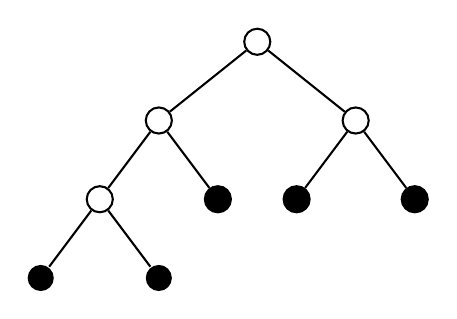
\begin{tikzpicture}
			\node [circle,draw]{} [level distance=10mm,sibling distance=25mm]
			child { node [circle,draw]{} [level distance=10mm ,sibling distance=15mm]
					child {node [circle,draw] {}
							child {node [circle,fill] {}}
							child {node [circle,fill]{}}}
					child {node [circle,draw,fill]{}}
				}
			child {node [circle,draw] {} [level distance=10mm ,sibling distance=15mm]
					child {node [circle,draw,fill] {}}
					child {node [circle,draw,fill]{}}
				};
		\end{tikzpicture}
	\end{center}
	\caption{L'albero binario $(((\emptyset, \emptyset), \emptyset), (\emptyset, \emptyset))$.}
	\label{fig:btree_example}
\end{figure}

\noindent
Ora stiamo descrivendo alberi \textit{vuoti}, ossia che non contengono dati:
alternative sono gli alberi \textbf{ancillari}, i quali contengono dati solo nei nodi interni
o solo nelle foglie. Al netto di queste distinzioni, definiamo $E$ l'insieme dei nodi
esterni, $I$ l'insieme dei nodi interni di un albero binario e $n$ il numero di nodi
interni, ossia $n = |I|$. Inoltre, `equipaggiamo' gli alberi binari di due funzioni
$ext$ e $int$, che denotano l'insieme delle foglie interne e l'insieme delle foglie
interne di un albero binario.

\begin{theorem} \label{thm:btree_leaves}
	In ogni albero binario, il numero di foglie in un albero binario è uguale al numero di nodi esterni più uno:
	$$
		|E| = |I| + 1
	$$
\end{theorem}
\begin{proof}
	Per induzione.
	\begin{itemize}
		\item{\bf base}: $ext(\emptyset) = 1$ e $int(\emptyset) = 0$.
		\item{\bf induzione}: siano $L, R$ due alberi binari. Allora
		$$
			ext((L,R)) = ext(L) + ext(R) = int(L) + 1 + int(R) + 1 = int((L, R))  + 1
		$$
	\end{itemize}
\end{proof}

\begin{corollario}
	Ogni albero con $n$ nodi interni ha in totale $2n +1$ nodi.
\end{corollario}

\begin{theorem}[di Catalan]\label{thm:catalan}
	Il numero di alberi binari con $n$ nodi interni è
	$$
		C_n = \frac{1}{n+1}{2n \choose n}
	$$
\end{theorem}
\begin{proof}
	Omessa.
\end{proof}
\begin{corollario}
	$ \forall n ~ \log_2(C_n)  =2n + O(\log_2(n)) $
\end{corollario}
\begin{proof}
	Utilizzando l'approssimazione di Stirling
	$$
		x! \approx \sqrt{2\pi x} (\frac{x}{e})^x
	$$

	si ha che
	$$
		C_n = \frac{1}{n+1} \frac{(2n)!}{n! (2n - n)!} = \frac{1}{n+1}\frac{(2n)!}{(n!)^2} \approx
		\frac{1}{n+1} \frac{\sqrt{4 \pi n} (\frac{2n}{e})^{2n}}{2 \pi n (\frac{n}{e})^{2n}}
		= \frac{1}{n+1} \frac{1}{\sqrt{\pi n }} 2^{2n} \approx \frac{4^n}{\sqrt{\pi n^3}}
	$$
	(che può essere dimostrato asintoticamente corretto).
	Questo significa che
	$$
		\log_2(C_n) = n \log_2(4) - \frac{1}{2}\log_2(\pi n^3)
		= 2n - \frac{3}{2}\log_2(n) - \frac{1}{2}\log_2(\pi)
		= 2n + O(\log_2(n))
	$$
\end{proof}
\begin{corollario}
	Per memorizzare alberi binari con $n$ nodi interni sono necessari
	$$
		Z_n = 2n + O(\log_2(n)) \text{ bit}
	$$
\end{corollario}

\subsection{L'ADT albero binario}
L'ADT che vogliamo costruire per un albero binario è definito a partire da una definizione
di nodi interni $I$, nodi interni $E$, e relazioni genitore-figlio. Le operazioni
che vogliamo eseguire su questi oggetti sono:
$$
	\forall n \in (I \cup E) ~~ \mathbf{is\_leaf}(n) = 1 \iff n \in  E
$$

$$
	\forall n \in (I \cup E) ~~ \mathbf{left\_child}(n) = \{n_l | n_l \text{ è il figlio sinistro di } n\}
$$

$$
	\forall n \in (I \cup E) ~~ \mathbf{right\_child}(n) = \{n_l | n_l \text{ è il figlio destro di } n\}
$$

$$
	\forall n \in (I \cup E) ~~ \mathbf{parent}(n) = \{p | n \text{ è il figlio di } p\}
$$


\subsubsection{Rappresentazione}
Per rappresentare un albero binario con $n$ nodi interni, numeriamo seguendo una visita in
ampiezza i nodi dell'albero, come rappresentato in \cref{fig:btree_rappr_num}. I numeri assegnati
andranno da $0$ a $2n$ e introducono una biiezione tra l'insieme $\{0, \cdots, 2n\}$ e i nodi,
realizzato come una funzione $node: \{0, \cdots, 2n\} \rightarrow (E \cup I)$.

\begin{figure}[h]
	\centering
	\begin{subfigure}[t]{0.45\textwidth}
		\centering
		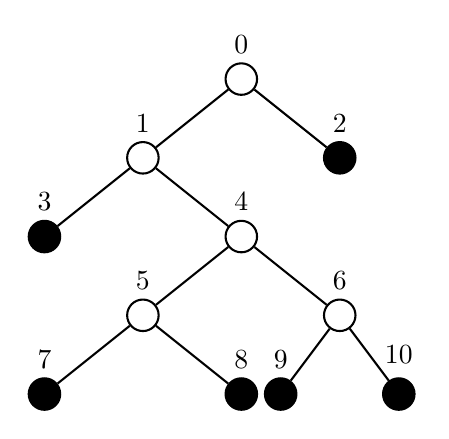
\begin{tikzpicture}[
				every node/.style={circle, draw, minimum size=4mm, inner sep=0.5mm},
				level distance=10mm,
				level 1/.style={sibling distance=25mm},
				level 2/.style={sibling distance=25mm}]
			\node [label=above:{0}]{}
			child {
			node [label=above:{1}] {}
			child {node[fill, label=above:{3}]{}}
			child {
			node[label=above:{4}]{}
			child {
			node [label=above:{5}]{}
			child {node[fill,label=above:{7}]{}}
			child {node[fill,label=above:{8}]{}}
			}
			child {
			node[label=above:{6}]  {}
			[level distance=10mm ,sibling distance=15mm]
			child {node[fill,label=above:{9}] {}}
			child {node[fill,label=above:{10}] {}}
			}
			}
			}
			child {node [fill, label=above:{2}]{}};
		\end{tikzpicture}

		\caption{L'albero binario $((\emptyset, ((\emptyset, \emptyset), (\emptyset, \emptyset))), \emptyset)$ numerato.}
		\label{fig:btree_rappr_num}

	\end{subfigure}
	\begin{subfigure}[t]{0.45\textwidth}
		\centering
		\tikzset{every picture/.style={line width=0.75pt}} %set default line width to 0.75pt        

		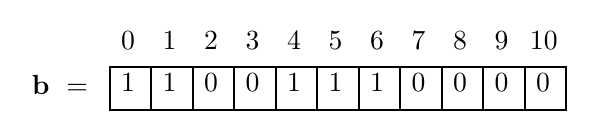
\begin{tikzpicture}[x=0.75pt,y=0.75pt,yscale=-1,xscale=1]
			%uncomment if require: \path (0,300); %set diagram left start at 0, and has height of 300

			%Shape: Rectangle [id:dp4589196649246813] 
			\draw   (160,120) -- (180,120) -- (180,140.67) -- (160,140.67) -- cycle ;
			%Shape: Rectangle [id:dp7482491218517459] 
			\draw   (180,120) -- (200,120) -- (200,140.67) -- (180,140.67) -- cycle ;
			%Shape: Rectangle [id:dp3055160865785119] 
			\draw   (200,120) -- (220,120) -- (220,140.67) -- (200,140.67) -- cycle ;
			%Shape: Rectangle [id:dp6460750266770654] 
			\draw   (220,120) -- (240,120) -- (240,140.67) -- (220,140.67) -- cycle ;
			%Shape: Rectangle [id:dp45180487257490853] 
			\draw   (240,120) -- (260,120) -- (260,140.67) -- (240,140.67) -- cycle ;
			%Shape: Rectangle [id:dp28629681352535363] 
			\draw   (260,120) -- (280,120) -- (280,140.67) -- (260,140.67) -- cycle ;
			%Shape: Rectangle [id:dp7936708770675233] 
			\draw   (280,120) -- (300,120) -- (300,140.67) -- (280,140.67) -- cycle ;
			%Shape: Rectangle [id:dp23915136536136594] 
			\draw   (300,120) -- (320,120) -- (320,140.67) -- (300,140.67) -- cycle ;
			%Shape: Rectangle [id:dp722227591081337] 
			\draw   (320,120) -- (340,120) -- (340,140.67) -- (320,140.67) -- cycle ;
			%Shape: Rectangle [id:dp6052306075858915] 
			\draw   (340,120) -- (360,120) -- (360,140.67) -- (340,140.67) -- cycle ;
			%Shape: Rectangle [id:dp5583026074292488] 
			\draw   (360,120) -- (380,120) -- (380,140.67) -- (360,140.67) -- cycle ;

			% Text Node
			\draw (121,122.4) node [anchor=north west][inner sep=0.75pt]    {$\mathbf{b} \ =\ $};
			% Text Node
			\draw (164,101.4) node [anchor=north west][inner sep=0.75pt]    {$0$};
			% Text Node
			\draw (184,101.4) node [anchor=north west][inner sep=0.75pt]    {$1$};
			% Text Node
			\draw (204,101.4) node [anchor=north west][inner sep=0.75pt]    {$2$};
			% Text Node
			\draw (224,101.4) node [anchor=north west][inner sep=0.75pt]    {$3$};
			% Text Node
			\draw (244,101.4) node [anchor=north west][inner sep=0.75pt]    {$4$};
			% Text Node
			\draw (264,101.4) node [anchor=north west][inner sep=0.75pt]    {$5$};
			% Text Node
			\draw (284,101.4) node [anchor=north west][inner sep=0.75pt]    {$6$};
			% Text Node
			\draw (304,101.4) node [anchor=north west][inner sep=0.75pt]    {$7$};
			% Text Node
			\draw (324,101.4) node [anchor=north west][inner sep=0.75pt]    {$8$};
			% Text Node
			\draw (344,101.46) node [anchor=north west][inner sep=0.75pt]    {$9$};
			% Text Node
			\draw (361,101.4) node [anchor=north west][inner sep=0.75pt]    {$10$};
			% Text Node
			\draw (164,121.4) node [anchor=north west][inner sep=0.75pt]    {$1$};
			% Text Node
			\draw (184,121.4) node [anchor=north west][inner sep=0.75pt]    {$1$};
			% Text Node
			\draw (204,121.4) node [anchor=north west][inner sep=0.75pt]    {$0$};
			% Text Node
			\draw (224,121.4) node [anchor=north west][inner sep=0.75pt]    {$0$};
			% Text Node
			\draw (244,121.4) node [anchor=north west][inner sep=0.75pt]    {$1$};
			% Text Node
			\draw (264,121.4) node [anchor=north west][inner sep=0.75pt]    {$1$};
			% Text Node
			\draw (284,121.4) node [anchor=north west][inner sep=0.75pt]    {$1$};
			% Text Node
			\draw (304,121.4) node [anchor=north west][inner sep=0.75pt]    {$0$};
			% Text Node
			\draw (324,121.4) node [anchor=north west][inner sep=0.75pt]    {$0$};
			% Text Node
			\draw (344,121.46) node [anchor=north west][inner sep=0.75pt]    {$0$};
			% Text Node
			\draw (364,121.4) node [anchor=north west][inner sep=0.75pt]    {$0$};

		\end{tikzpicture}
		\caption{Vettore $\mathbf{v}$ associato.}
		\label{fig:btree_rappr_vec}
	\end{subfigure}
	\caption{Un albero binario e il suo vettore associato.}
\end{figure}
\noindent
La concreta rappresentazione dell'albero si realizza con un vettore di bit di lunghezza
$2n + 1$ $\mathbf{v}$ tale che
$$
	\forall i \in \{0, \cdots, 2n\} ~~ \mathbf{v}[i] =
	\begin{cases}
		1 & node(i) \in I \\
		0 & node(i) \in E
	\end{cases}
$$
ottenendo quindi esattamente $n$ `$1$' nel vettore, come mostrato in \cref{fig:btree_rappr_vec}.

\subsubsection{Implementazione}
Per capire come implementare l'ADT utilizzando il vettore $\mathbf{v}$, ci poniamo
nella situazione di dover trovare, dato un nodo numerato $p$ in un albero
binario $T$, i suoi due figli, i quali sono numerati $q$ e $q+1$.
Sia quindi $T'$ un sottoalbero di $T$, radicato nella stessa radice di $T$,
che contiene tutti i nodi di $T$ numerati fino al nodo precedente
al nodo $q$, come rappresentato in \cref{fig:btree_rappr_step}.


\begin{figure}[h]
	\centering



	\tikzset{every picture/.style={line width=0.75pt}} %set default line width to 0.75pt        

	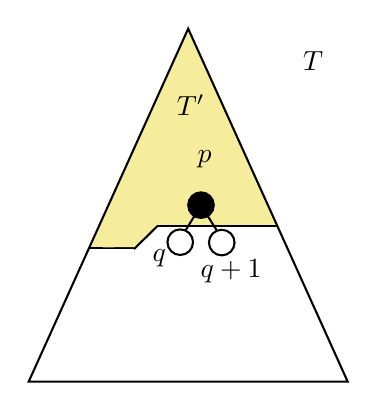
\begin{tikzpicture}[x=0.75pt,y=0.75pt,yscale=-1,xscale=1]
		%uncomment if require: \path (0,539); %set diagram left start at 0, and has height of 539

		%Shape: Trapezoid [id:dp3557987154319203] 
		\draw  [color={rgb, 255:red, 246; green, 237; blue, 156 }  ,draw opacity=1 ][fill={rgb, 255:red, 246; green, 237; blue, 156 }  ,fill opacity=1 ] (312.92,126.04) -- (317.75,115.9) -- (328.33,115.9) -- (333.17,126.04) -- cycle ;
		%Shape: Right Triangle [id:dp7862842021574125] 
		\draw  [color={rgb, 255:red, 246; green, 237; blue, 156 }  ,draw opacity=1 ][fill={rgb, 255:red, 246; green, 237; blue, 156 }  ,fill opacity=1 ] (346,114.3) -- (334.2,125.7) -- (334.2,114.3) -- cycle ;
		%Shape: Triangle [id:dp9413454407809129] 
		\draw  [color={rgb, 255:red, 246; green, 237; blue, 156 }  ,draw opacity=1 ][fill={rgb, 255:red, 246; green, 237; blue, 156 }  ,fill opacity=1 ] (360.11,21.08) -- (402.87,115.9) -- (317.34,115.9) -- cycle ;
		%Shape: Circle [id:dp7169355320482411] 
		\draw  [fill={rgb, 255:red, 0; green, 0; blue, 0 }  ,fill opacity=1 ] (360.11,106.08) .. controls (360.11,102.68) and (362.87,99.92) .. (366.28,99.92) .. controls (369.68,99.92) and (372.44,102.68) .. (372.44,106.08) .. controls (372.44,109.49) and (369.68,112.25) .. (366.28,112.25) .. controls (362.87,112.25) and (360.11,109.49) .. (360.11,106.08) -- cycle ;
		%Straight Lines [id:da11031799115386731] 
		\draw    (366.28,106.08) -- (356.04,122.86) ;
		%Straight Lines [id:da5314879825236313] 
		\draw    (366.28,106.08) -- (376.09,121.82) ;
		%Shape: Triangle [id:dp2636274720755136] 
		\draw   (360.11,21.08) -- (436.94,191.08) -- (283.28,191.08) -- cycle ;
		%Straight Lines [id:da07107046785599602] 
		\draw    (312.18,126.95) -- (334.47,126.95) ;
		%Straight Lines [id:da23996966123276942] 
		\draw    (345.08,116.14) -- (402.93,116.14) ;
		%Straight Lines [id:da8657897153449609] 
		\draw    (345.49,115.99) -- (333.99,127.24) ;
		%Shape: Circle [id:dp6390655913899737] 
		\draw  [fill={rgb, 255:red, 255; green, 255; blue, 255 }  ,fill opacity=1 ] (350.11,123.93) .. controls (350.11,120.53) and (352.87,117.76) .. (356.28,117.76) .. controls (359.68,117.76) and (362.44,120.53) .. (362.44,123.93) .. controls (362.44,127.34) and (359.68,130.1) .. (356.28,130.1) .. controls (352.87,130.1) and (350.11,127.34) .. (350.11,123.93) -- cycle ;
		%Shape: Circle [id:dp31674144349432576] 
		\draw  [fill={rgb, 255:red, 255; green, 255; blue, 255 }  ,fill opacity=1 ] (370.11,124.11) .. controls (370.11,120.71) and (372.87,117.95) .. (376.28,117.95) .. controls (379.68,117.95) and (382.44,120.71) .. (382.44,124.11) .. controls (382.44,127.52) and (379.68,130.28) .. (376.28,130.28) .. controls (372.87,130.28) and (370.11,127.52) .. (370.11,124.11) -- cycle ;
		%Shape: Right Triangle [id:dp4307506900461393] 
		\draw  [color={rgb, 255:red, 246; green, 237; blue, 156 }  ,draw opacity=1 ][fill={rgb, 255:red, 246; green, 237; blue, 156 }  ,fill opacity=1 ] (320.12,125.88) -- (333.92,109.62) -- (333.95,125.85) -- cycle ;

		% Text Node
		\draw (341.53,125.76) node [anchor=north west][inner sep=0.75pt]    {$q$};
		% Text Node
		\draw (364.58,131.05) node [anchor=north west][inner sep=0.75pt]    {$q+1$};
		% Text Node
		\draw (363.18,78.26) node [anchor=north west][inner sep=0.75pt]    {$p$};
		% Text Node
		\draw (353.2,51.2) node [anchor=north west][inner sep=0.75pt]    {$T'$};
		% Text Node
		\draw (414,30.4) node [anchor=north west][inner sep=0.75pt]    {$T$};


	\end{tikzpicture}
	\caption{Sottoalbero $T'$ di $T$ utilizzato per calcolare $q$ e $q+1$.}
	\label{fig:btree_rappr_step}
\end{figure}

Definiamo l'insieme dei nodi interni di $T$ con numerazione strettamente
minore di $p$
$$
	E_{T, p} = \{n \in int(T) | n < p \}
$$
e, intuitivamente, deve essere
$$
	q = |int(T')| + |ext(T')| = 2 |int(T')| + 1 = 2 |E_{T,p}| + 1 = 2 \mathbf{rank_v}(p) + 1
$$
poiché $|E_{T,p}|$ è uguale al numero di `$1$' presenti in $\mathbf{v}$ con indice
strettamente minore a $p$, concludendo, chiaramente se e solo se
$\mathbf{is\_leaf}(p) = \mathbf{v}[p] = 1$, che\footnote{In quanto segue si omette
	la biiezione $node$, dando per implicito il rapporto tra enumerazione e nodi.}
$$
	\forall p \in \{0, \cdots, 2n\} ~~ \mathbf{left\_child}(p) = 2 \mathbf{rank_v}(p) + 1
$$
$$
	\forall p \in \{0, \cdots, 2n\} ~~ \mathbf{right\_child}(p) = 2 \mathbf{rank_v}(p) + 2
$$
Per risalire al genitore a partire da un figlio, ossia da $q$ risalire a $p$,
basta osservare che $p$ è un nodo tale per cui
$$
	\begin{cases}
		2\mathbf{rank_v}(p) + 1 = q & \text{se } q \text{ è il figlio di sinistra} \\
		2\mathbf{rank_v}(p) + 2 = q & \text{se } q \text{ è il figlio di destra}
	\end{cases}
	\implies
	\begin{cases}
		\mathbf{rank_v}(p) + \frac{1}{2} = \frac{q}{2} \\
		\mathbf{rank_v}(p) + 1 = \frac{q}{2}
	\end{cases}
	\implies
	\begin{cases}
		\mathbf{rank_v}(p) = \frac{q}{2}  - \frac{1}{2} \\
		\mathbf{rank_v}(p) = \frac{q}{2} - 1
	\end{cases}
$$
ma possiamo concludere che
$$
	\mathbf{rank_v}(p) = \lfloor \frac{q}{2} - \frac{1}{2} \rfloor
$$
siccome a seconda che $q$ sia pari o dispari l'equazione sarà sempre verificata,
ossia questa uguaglianza è vera se e solo se è almeno una delle due precedenti;
se $\frac{q}{2} - \frac{1}{2}$ è intero, allora è vera la prima equazione, mentre
se non è intero si ottiene $\frac{q}{2} - 1$, verificando la seconda.
Applichiamo ad entrami i membri l'operazione di $\mathbf{select}$:
$$
	\mathbf{select_v(rank_v}(p)) = \mathbf{select_v}(\lfloor \frac{q}{2} - \frac{1}{2} \rfloor)
	\implies p = \mathbf{select_v}(\lfloor \frac{q}{2} - \frac{1}{2} \rfloor)
$$

\subsubsection{Complessità in spazio}
Per rappresentare un albero con $n$ nodi interni utilizziamo un vettore $b$ che ha tanti
bit tanti quanti sono i nodi dell'albero, ossia $2n +1$. Oltre a questo, si utilizza
lo spazio utilizzato dalle strutture di rank e select, ossia
$$
	D_n = 2n +1 + o(2n+1) = 2n + 1 + o(n)
$$
con un risultato per $Z_n$ pari a $2n + O(\log_1(n))$, la differenza è
$$
	D_n - Z_n = o(n)
$$
pertanto la struttura è succinta con accesso in tempo costante.

\subsubsection{Alberi binari con dati}
Se i dati si trovano su ogni tipo di nodo dell'albero (sia interni che interni) i dati
ancillari si possono mantenere in un ulteriore vettore della stessa lunghezza.
Se, invece, i dati ancillari si trovano esclusivamente sui nodi interni,
la situazione è leggermente più complicata: il vettore dei dati avrà
lunghezza pare ai al numero di nodi interni e sarà necessario ottenere il numero
ordinale del nodo interno, utilizzando quindi la funzione rank.
Alternativamente, se si vogliono salvare dati sulle foglie, si dovrà utilizzare
una tecnica in grado di contare il \texttt{rank} per gli $0$.

\section{Struttura di Elias-Fano per sequenze monotone}
La struttura (o codifica, rappresentazione) di Elias-Fano che andiamo
a presentare si occupa delle sequenze monotone di interi, ossia
delle sequenze di $n$ numeri interi
$$
	0 \leq x_0, x_1, \cdots, x_{n+1}
$$
ordinati, ossia
$$
	\forall i, j ~ i < j \implies x_i < x_j
$$
e tali per cui
$$
	\exists u ~ \forall i ~ x_i < u
$$
dove $u$ è chiamato \textit{dimensione dell'universo}.
L'ADT che vogliamo rappresentare richiede una primitiva
che, presentato un indice $i$, restituisce l'$i$-esimo elemento della sequenza,
ossia
$$
	\forall i ~ \mathbf{project}(i) = x_i
$$
La rappresentazione di sequenze monotone di interi è molto utile.
Per esempio, per rappresentare un grafo, si può attribuire ad ogni
nodo un numero: l'idea classica è quella di utilizzare poi, per esempio,
liste di adiacenza per elencare i nodi raggiungibili da un certo noto
considerato. I nodi adiacenti possono essere ordinati in ordine crescente,
ottenendo una sequenza esattamente monotona.
Un altro esempio di utilizzo di sequenze monotone è negli indici inversi.


\subsection{Rappresentazione}
La rappresentazione banale sarebbe utilizare un vettore di $n$ numeri
utilizzando per ognuno $\log_2(u)$ bit; la rappresentazione di Elias-Fano
utilizza meno spazio basandosi sulla seguente idea: si definisce
$$
	l = \max\{0, \lfloor\log_2(\frac{u}{n})\rfloor\}
$$
e gli $l$ bit meno significativi di ogni $x_i$ vengono salvati
esplicitamente, mentre i rimanenti bit vengono rappresentati
in un altro modo. Consideremo sempre il caso in cui $l\neq 0$, in
quanto $l = 0 \iff u < n$, facendo quindi una moderata
assunzione di sparsità.
\begin{table}[h]
	\centering
	\begin{tabular}{c}
		\begin{lstlisting}
	 0 0 0 1 parte superiore
	 . . . .
	 1 1 1 1 		
	 ------- limite l 
	 0 1 1 1 			
	 . . . .
	 1 0 0 1 parte inferiore
    \end{lstlisting}
	\end{tabular}
	\caption{Divisione di ogni $x_i$.}
\end{table}

\subsubsection{Implementazione e complessità in spazio}
Le parti inferiori vengono `estratte' definendo
$$
	\forall i \in \{0, \cdots, n\} ~ l_i = x_i \mod 2^l
$$
utilizzando $n \cdot l$ bit in totale.  Ciò che rimane è la parte superiore, ossia
$s_i = \lfloor{\frac{x_{i}}{2^l}}\rfloor$; definiamo una sequenza di differenze
$$
	d_i = \lfloor{\frac{x_i}{2^l}}\rfloor - \lfloor{\frac{x_{i-1}}{2^l}}\rfloor
$$
assumendo $x_{-1} = 0$. Stiamo sfruttando il fatto che la sequenza sia non
decrescente, quindi $\forall i ~ d_i \geq 0$.

Ogni differenza della sequenza viene rappresentata in unario, utilizzando $d_i$ bit
`$0$' seguiti dal bit `$1$' per rappresentare il valore $d_i$; la sequenza
così rappresentata viene salvata in un vettore $\mathbf{d}$ equipaggiato
con funzioni di rango e selezione. Questa struttura occupa in spazio
una quantità al più
$$
	\sum_{i = 0}^{n - 1}(d_i + 1) = n + \sum_{i=0}^{n-1} d_i
	= n + \sum_{i = 0}^{n-1} (\lfloor{\frac{x_i}{2^l}}\rfloor - \lfloor{\frac{x_{i-1}}{2^l}}\rfloor) \text{ bit}
$$
che identifica una serie telescopica; pertanto, il consumo in spazio è
$$
	n + (\lfloor{\frac{x_{n-1}}{2^l}}\rfloor -\lfloor{\frac{x_{-1}}{2^l}}\rfloor) \leq n + \frac{u}{2^l}
	= n + \frac{u}{2^{\lfloor \log_2(\frac{u}{n})\rfloor}} \text{ bit}
$$
Se $u/n$ è una potenza di $2$, allora il consumo è
$$
	n + \frac{u}{(u/n)} = 2n \text{ bit}
$$
altrimenti è al più
$$
	n + \frac{u}{2^{\log_2(\frac{u}{n}) - 1 }} = n + \frac{u}{2^{\log_2(u/n)}1/2} = n + \frac{2n}{u/n} = 3n \text{ bit}
$$
Considerando entrambe le parti, questa struttura occupa in spazio $l\cdot n$ bit
per la parte inferiore e $2n$ o $3n$ bit per la parte superiore; in totale,
quindi, si consumano $(l+2)n$ o $(l+3)n$ bit.
Ricordando che stiamo considerando sempre $l = \lfloor \log_2(u/n) \rfloor$, consideriamo
$$
	\lceil \log_2(u/n) \rceil =
	\begin{cases}
		l & u/n \text{ è una potenza di } 2 \\
		l +1                                \\
	\end{cases}
$$
e concludiamo
$$
	D_n = (2 + \lceil \log_2(u/n) \rceil) n \text{ bit}
$$
che però non tiene conto dello spazio occupato dalla struttura di rango e selezione,
che infatti sono necessarie: supponiamo di volere la posizione dell'$i$-esimo $1$ in $\mathbf{d}$:
\begin{align*}
	\mathbf{select_d}(i) = d_0 + d_1 + \cdots + d_{i-1} + i & "i" \text{ è il numero di '1' in mezzo ai valori}
\end{align*}
quindi
$$
	\mathbf{select_d}(i) - i = \sum_{j = 0}^i \lfloor{\frac{x_{j}}{2^l}}\rfloor -\lfloor{\frac{x_{j-1}}{2^l}}\rfloor = \lfloor \frac{x_i}{2^l} \rfloor
$$
di conseguenza
$$
	x_i =  \lfloor \frac{x_i}{2^l} \rfloor 2^l + (x_i ~ \mathrm{mod} {2^l}) = (\mathbf{select_d}(i) - i ) 2^l + l_i
$$
Contando anche le strutture di rank e select, che quindi sono necessarie, si occupa uno spazio
$$
	D_n = (2 + \lceil \log_2(u/n) \rceil)n + o(n) \text{ bit}
$$

\subsection{Lower bound per le strutture di Elias-Fano}
La parte difficile dello studio di questa struttura è il calcolo del lower bound:
dobbiamo considerare tutte le sequenze monotone
$$
	0 \leq x_0 \leq \cdots \leq x_{n-1} \le u
$$
Quante sono, una volta fissati $n$ e $u$? Esse sono in biiezione con i multinsiemi di cardinalità
$n$ sottoinsiemi di $\{0,1, \cdots, u-1\}$. Uno di questi multinsiemi si può vedere come
$$
	c_0, c_1, \cdots, c_{u-1}
$$
dove ogni $c_i$ è il numero di occorrenze del valore $i$ nel multinsieme, ossia
il numero di soluzioni intere non negative dell'equazione
$$
	c_0 + c_1, \cdots, c_{u-1} = n
$$
e possiamo calcolare il numero di sequenze monotone calcolando il numero
di possibili soluzioni per questa equazione fissati $n$ e $u$.

Per esempio, si immagini di avere un universo di dimensione $u = 7$ e $n = 5$ numeri
estratti da $\{0, 1, \cdots, 7\}$: la sequenza
$$
	0 \leq 1 \leq 3 \leq 3 \leq 5 \leq 6 \le 7
$$
la cui equazione associata è
$$
	c_0 + c_1 + c_2 + \cdots + c_6 = 5
$$
è rappresentabile, in termini di $c_i$, come
$$
	c_0 = 0, c_1 = 1, c_2 = 0, c_3 = 2, c_4 = 0, c_5 = 1, c_6 = 1
$$
che è una soluzione dell'equazione precedente.

\subsubsection{Metodo stars and bars}
Per contare le possibili soluzioni si può utilizzare la tecnica \textit{stars and bars}, in
cui si utilizzano delle stringhe costruite utilizzando $n$ stelline e $u-1$ barrette, piazzate
in qualsiasi posizione:
$$
	| \star || \star \star || \star | \star
$$

Il numero di soluzioni è uguale al numero di stringhe costruite in tale modo: i valori nella sequenza
sono $n$ e vanno `distribuiti' in $u$ spazi, delineati dalle $u-1$ barrette. L'interpretazione della
stringa appena mostrata è $ c_0 = 0, c_1 = 1, c_2 = 0, c_3 = 2, c_4 = 0, c_5 = 1, c_6 = 1 $, come
nell'esempio precedente. I simboli utilizzabili sono $(u-1) + n$, pertanto le possibili stringhe
costruibili con questi simboli sono  ${u + n -1}\choose{u - 1}$.
Questo fornisce il lower bound desiderato:
$$
	Z_n = \log_2{{u + n -1}\choose{u - 1}} = \log_2{{u + n - 1}\choose{n}} \text{ bit}
$$
e introduciamo l'approssimazione
$$
	{{a}\choose{b}} \approx b \log_2(\frac{a}{b}) + (a - b)\log_2(\frac{a}{a-b})
$$
che ci permette di scrivere
\begin{align*}
	Z_n = \log_2{{u + n -1}\choose{u - 1}} & \approx n \log_2(\frac{u + n -1}{n}) + (u -1) \log_2(\frac{u + n - 1}{u - 1}) =        \\
	                                       & = n \log_2(\frac{u + n - 1}{n}) = n \log_2(\frac{u}{n}(1 + \frac{n}{u} - \frac{1}{u})) \\
	                                       & = n \log_2(\frac{u}{n}) + n \log_2(1 + \frac{n}{u} - \frac{1}{u}) \text{ bit}
\end{align*}

\noindent
Un'altra proprietà che utilizziamo è
$$
	x \approx \ln(1 + x)
$$
quindi
\begin{align*}
	Z_n & = n \log_2(\frac{u}{n}) + n \ln(1 + \frac{n}{u}-\frac{1}{u})\frac{1}{\ln(2)}
	\approx n \log_2(\frac{u}{n}) + n (\frac{n}{u}-\frac{1}{u})\frac{1}{\ln(2)}               \\
	    & = n \log_2(\frac{u}{n}) + \frac{1}{u}\frac{1}{\ln(2)} - \frac{n}{u}\frac{1}{\ln(2)}
	\approx n \log_2(\frac{u}{n}) \text{ bit}
\end{align*}

L'utilizzo in spazio calcolato precedentemente è
$$
	D_n = 2n + n \lceil \log_2(\frac{u}{n}) \rceil + o(n)
$$
In questo frangente, per raffinare l'analisi, conviene considerare la differenza
col lower bound non sull'intera struttura, bensì sul singolo elemento.
Definiamo, quindi, il lower bound per l'elemento
$$
	\bar{Z_n} \approx \log_2(\frac{u}{n})
$$
e
$$
	\bar{D_n} = 2+ \lceil \log_2(\frac{u}{n}) \rceil + o(n) = \bar{Z_n} + O(1)
$$
la struttura è `quasi' implicita, dove l'incertezza deriva dal numero di
approssimazioni fatte e sull'assunzione di sparsità; in pratica, ciò che succede
in pratica è che questa uguaglianza vale quando $n \leq \sqrt{u}$.

\section{Struttura per parentesi ben formate}
\subsection{Linguaggi di Dyck}
Un linguaggio di Dyck $L$ è un linguaggio sull'alfabeto $D=\{(,)\}$ tale che $L \subseteq D^*$
e una stringa $w \in D^*$ appartiene a $L$ se e solo se
\begin{enumerate}
	\item $|w|_{(} = |w|_{)}$; e
	\item $\forall w_1, w_2 \text{ tali che } w = w_1w_2 \implies|w_1|_{(} \geq |w_2|_{)}$
\end{enumerate}
Un modo interessante per studiare una parola $w$ di Dyck è studiarne la
\textit{funzione di eccesso}, definita
$$
	E_w(i) = |\{j | j \le i ~ w_j = ( ~\}| - |\{j | j \leq i ~ w_j = ) ~\}|
$$
\begin{figure}[h]
	\centering
	\begin{tikzpicture}
		\draw[->] (-1, 0) -- (8.50, 0) node[right] {$x$};
		\draw[->] (-1, 0) -- (-1, 4) node[above] {$y$};

		\draw (0,0) node[circle,fill,inner sep=1pt, label=above:{(}] {} -- (1,1) node[circle,fill,inner sep=1pt]{};
		\draw (1,1) node[circle,fill,inner sep=1pt, label=above:{(}] {} -- (2,1) node[circle,fill,inner sep=1pt]{};
		\draw (2,1) node[circle,fill,inner sep=1pt, label=above:{)}] {} -- (3,1) node[circle,fill,inner sep=1pt]{};
		\draw (3,1) node[circle,fill,inner sep=1pt, label=above:{(}] {} -- (4,2) node[circle,fill,inner sep=1pt]{};
		\draw (4,2) node[circle,fill,inner sep=1pt, label=above:{(}] {} -- (5,2) node[circle,fill,inner sep=1pt]{};
		\draw (5,2) node[circle,fill,inner sep=1pt, label=above:{)}] {} -- (6,1) node[circle,fill,inner sep=1pt]{};
		\draw (6,1) node[circle,fill,inner sep=1pt, label=above:{)}] {} -- (7,0) node[circle,fill,inner sep=1pt, label=above:{)}]{};
	\end{tikzpicture}
	\caption{Funzione di eccesso per la parola $(()(()))$.}
	\label{fig:func_excess}
\end{figure}

Questa funzione parte da $0$, può tornare a $0$ e, se la parola è effettivamente nel
linguaggio, termina a $0$. Ci sono due tipi di stringhe di Dyck: quelle per cui
la funzione non raggiunge nessuno $0$ tranne quello iniziale e quello finale,
chiamate \textit{fortemente bilanciate}, e quelle per cui questa funzione raggiunge
uno $0$ diverso da quello iniziale e quello finale, quindi $w = w_1w_2$ è
\textit{debolmente bilanciata} e tale per cui almeno uno tra $w_1$ e $w_2$ è
fortemente bilanciata.

Ci sono molti motivi per cui le sequenze di parentesi sono interessanti. In particolare,
le espressioni ben parentesizzate sono in biiezione sia con le foreste di alberi binari che con gli
alberi non binari. In qualche modo, esattamente come abbiamo visto una rappresentazione
per gli alberi binari in precedenza, ora stiamo analizzando una struttura per alberi
generali. Le sequenze di parentesi aperte e chiuse le penseremo come stringhe di bit, cioè
una stringa
$$
	(()(()())(()))
$$
è rappresentata come una stringa
$$
	11011010011000
$$
la cui funzione di eccesso è rappresentata in \cref{fig:func_excess_example}.

\begin{figure}[h]
	\centering
	\begin{tikzpicture}
		\draw[->] (-1, 0) -- (14.5, 0) node[right] {$x$};
		\draw[->] (-1, 0) -- (-1, 4) node[above] {$y$};

		\draw (0,0) node[label=above:{(}]	{} -- 	(1,1) node[circle,fill,inner sep=1pt]{};
		\draw (1,1) node[label=above:{(}] 	{} -- 	(2,1) node[circle,fill,inner sep=1pt]{};
		\draw (2,1) node[label=above:{)}] 	{} -- 	(3,1) node[circle,fill,inner sep=1pt]{};
		\draw (3,1) node[label=above:{(}] 	{} -- 	(4,2) node[circle,fill,inner sep=1pt]{};
		\draw (4,2) node[label=above:{(}] 	{} -- 	(5,2) node[circle,fill,inner sep=1pt]{};
		\draw (5,2) node[label=above:{)}] 	{} -- 	(6,2) node[circle,fill,inner sep=1pt]{};
		\draw (6,2) node[label=above:{(}] 	{} -- 	(7,2) node[circle,fill,inner sep=1pt]{};
		\draw (7,2) node[label=above:{)}] 	{} -- 	(8,1) node[circle,fill,inner sep=1pt]{};
		\draw (8,1) node[label=above:{)}] 	{} -- 	(9,1) node[circle,fill,inner sep=1pt]{};
		\draw (9,1) node[label=above:{(}] 	{} -- 	(10,2) node[circle,fill,inner sep=1pt]{};
		\draw (10,2) node[label=above:{(}]  	{} -- 	(11,2) node[circle,fill,inner sep=1pt]{};
		\draw (11,2) node[label=above:{)}]  	{} -- 	(12,1) node[circle,fill,inner sep=1pt]{};
		\draw (12,1) node[label=above:{)}]  	{} -- 	(13,0) node[circle,fill,inner sep=1pt,label=above:{)}]{};
	\end{tikzpicture}
	\caption{Funzione di eccesso per la parola $(()(()())(()))$.}
	\label{fig:func_excess_example}
\end{figure}

\subsection{L'ADT stringa bilanciata}
L'ADT che vogliamo descrivere per le stringhe di parentesi ben bilanciate ha le primitive
$$
	\forall p \in \mathbb{N} ~~ \mathbf{find\_open}(p) = \text{parentesi aperta corrispondente alla chiusa in posizione } p
$$
$$
	\forall p \in \mathbb{N} ~~ \mathbf{find\_close}(p) = \text{parentesi chiusa corrispondente all'aperta in posizione } p
$$
$$
	\forall p \in \mathbb{N} ~~ \mathbf{enclose}(p) = \text{prima parentesi aperta che racchiude la parentesi in posizione } p
$$

Pensando ad una soluzione banale, una $\mathbf{find\_open}$ in una qualche posizione si può
calcolare innanzitutto realizzando che la parentesi aperta corrispondente ad una
parentesi chiusa è sicuramente prima della chiusa stessa; basta quindi cercare all'indietro fermandosi
alla prima parentesi aperta che ha la stessa funzione di eccesso. Analogamente si fa per $\mathbf{find\_close}$.
La cosa più semplice, quindi, sarebbe calcolare anticipatamente la funzione di eccesso e usarla
facendo ricerche lineari, utilizzando uno spazio $n \log_2(n)$.
Faremo meglio creando una struttura compatta con tempo di interrogazione logaritmico.

\subsubsection{Rappresentazione}
La prima operazione sulle parentesi da eseguire nella costruzione della struttura è dividere, nuovamente,
la parola in blocchi di lunghezza $l$, creando $k = \lceil n/l \rceil$ blocchi. In ogni blocco
ci sono parentesi chiuse e aperte e, in alcuni casi, le parentesi hanno la loro corrispondente
dentro il blocco stesso: in questa situazione, definiamo la parentesi \textit{vicina}, mentre
tutte le altri sono definite \textit{lontane}; in generale, tutte le parentesi aperte lontane
si chiuderanno in un qualche blocco successivo.

In ogni blocco ci sono alcune parentesi vicine e varie parentesi lontane. Può succedere
che una o più parentesi lontane si chiudano nello stesso blocco: definiamo \textit{pioniera}
la lontana aperta (benché si possa fare lo stesso ragionamento, a specchio, per le chiuse)
che è la prima del blocco al quale appartiene a chiudersi in un qualsiasi altro blocco successivo.
Un esempio di queste divisioni è in \cref{fig:paren_blocks}, dove le parentesi gialle sono le vicine,
quelle blu sono lontane e quelle rosse sono pioniere.

\begin{figure}[h]

	\centering

	\tikzset{every picture/.style={line width=0.75pt}} %set default line width to 0.75pt        

	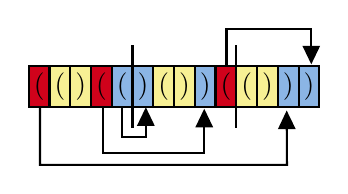
\begin{tikzpicture}[x=0.75pt,y=0.75pt,yscale=-1,xscale=1]
		%uncomment if require: \path (0,300); %set diagram left start at 0, and has height of 300

		%Shape: Rectangle [id:dp12028039856705786] 
		\draw  [fill={rgb, 255:red, 208; green, 2; blue, 27 }  ,fill opacity=1 ] (160,170) -- (170,170) -- (170,190) -- (160,190) -- cycle ;

		%Shape: Rectangle [id:dp6017350169887977] 
		\draw  [fill={rgb, 255:red, 247; green, 240; blue, 148 }  ,fill opacity=1 ] (170,170) -- (180,170) -- (180,190) -- (170,190) -- cycle ;

		%Shape: Rectangle [id:dp1862637830525412] 
		\draw  [fill={rgb, 255:red, 247; green, 240; blue, 148 }  ,fill opacity=1 ] (180,170) -- (190,170) -- (190,190) -- (180,190) -- cycle ;

		%Shape: Rectangle [id:dp7375538410378665] 
		\draw  [fill={rgb, 255:red, 208; green, 2; blue, 27 }  ,fill opacity=1 ] (190,170) -- (200,170) -- (200,190) -- (190,190) -- cycle ;

		%Shape: Rectangle [id:dp42832713437851455] 
		\draw  [fill={rgb, 255:red, 139; green, 181; blue, 229 }  ,fill opacity=1 ] (200,170) -- (210,170) -- (210,190) -- (200,190) -- cycle ;

		%Shape: Rectangle [id:dp3771120606312378] 
		\draw  [fill={rgb, 255:red, 139; green, 181; blue, 229 }  ,fill opacity=1 ] (210,170) -- (220,170) -- (220,190) -- (210,190) -- cycle ;

		%Shape: Rectangle [id:dp19892421904849122] 
		\draw  [fill={rgb, 255:red, 247; green, 240; blue, 148 }  ,fill opacity=1 ] (220,170) -- (230,170) -- (230,190) -- (220,190) -- cycle ;

		%Shape: Rectangle [id:dp0006276055923941648] 
		\draw  [fill={rgb, 255:red, 247; green, 240; blue, 148 }  ,fill opacity=1 ] (230,170) -- (240,170) -- (240,190) -- (230,190) -- cycle ;

		%Shape: Rectangle [id:dp16538357452442487] 
		\draw  [fill={rgb, 255:red, 139; green, 181; blue, 229 }  ,fill opacity=1 ] (240,170) -- (250,170) -- (250,190) -- (240,190) -- cycle ;

		%Shape: Rectangle [id:dp06112380309966958] 
		\draw  [fill={rgb, 255:red, 208; green, 2; blue, 27 }  ,fill opacity=1 ] (250,170) -- (260,170) -- (260,190) -- (250,190) -- cycle ;

		%Shape: Rectangle [id:dp06951356935410424] 
		\draw  [fill={rgb, 255:red, 247; green, 240; blue, 148 }  ,fill opacity=1 ] (260,170) -- (270,170) -- (270,190) -- (260,190) -- cycle ;

		%Shape: Rectangle [id:dp885838800749071] 
		\draw  [fill={rgb, 255:red, 247; green, 240; blue, 148 }  ,fill opacity=1 ] (270,170) -- (280,170) -- (280,190) -- (270,190) -- cycle ;

		%Shape: Rectangle [id:dp37752499309076915] 
		\draw  [fill={rgb, 255:red, 139; green, 181; blue, 229 }  ,fill opacity=1 ] (280,170) -- (290,170) -- (290,190) -- (280,190) -- cycle ;

		%Shape: Rectangle [id:dp7109616333523956] 
		\draw  [fill={rgb, 255:red, 139; green, 181; blue, 229 }  ,fill opacity=1 ] (290,170) -- (300,170) -- (300,190) -- (290,190) -- cycle ;

		%Straight Lines [id:da856450147041028] 
		\draw    (210,160) -- (210,200) ;
		%Straight Lines [id:da0823905364290688] 
		\draw    (260,160) -- (260,200) ;
		%Straight Lines [id:da8657156752341498] 
		\draw    (205.14,190.29) -- (205.14,204.36) -- (216.43,204.36) -- (216.43,192.93) ;
		\draw [shift={(216.43,189.93)}, rotate = 90] [fill={rgb, 255:red, 0; green, 0; blue, 0 }  ][line width=0.08]  [draw opacity=0] (8.93,-4.29) -- (0,0) -- (8.93,4.29) -- cycle    ;
		%Straight Lines [id:da4613663625082196] 
		\draw    (195.57,189.79) -- (195.57,212.07) -- (244.57,212.07) -- (244.57,193.64) ;
		\draw [shift={(244.57,190.64)}, rotate = 90] [fill={rgb, 255:red, 0; green, 0; blue, 0 }  ][line width=0.08]  [draw opacity=0] (8.93,-4.29) -- (0,0) -- (8.93,4.29) -- cycle    ;
		%Straight Lines [id:da9063548393327128] 
		\draw    (165.43,190.21) -- (165.43,217.64) -- (284.43,217.64) -- (284.3,194.5) ;
		\draw [shift={(284.29,191.5)}, rotate = 89.69] [fill={rgb, 255:red, 0; green, 0; blue, 0 }  ][line width=0.08]  [draw opacity=0] (8.93,-4.29) -- (0,0) -- (8.93,4.29) -- cycle    ;
		%Straight Lines [id:da09579212789908009] 
		\draw    (255.29,170.21) -- (255.29,152.07) -- (296.14,152.07) -- (296.14,166.21) ;
		\draw [shift={(296.14,169.21)}, rotate = 270] [fill={rgb, 255:red, 0; green, 0; blue, 0 }  ][line width=0.08]  [draw opacity=0] (8.93,-4.29) -- (0,0) -- (8.93,4.29) -- cycle    ;

		% Text Node
		\draw (161,172) node [anchor=north west][inner sep=0.75pt]   [align=left] {(};
		% Text Node
		\draw (171,172) node [anchor=north west][inner sep=0.75pt]   [align=left] {(};
		% Text Node
		\draw (181,172) node [anchor=north west][inner sep=0.75pt]   [align=left] {)};
		% Text Node
		\draw (211,172) node [anchor=north west][inner sep=0.75pt]   [align=left] {)};
		% Text Node
		\draw (201,172) node [anchor=north west][inner sep=0.75pt]   [align=left] {(};
		% Text Node
		\draw (191,172) node [anchor=north west][inner sep=0.75pt]   [align=left] {(};
		% Text Node
		\draw (271,172) node [anchor=north west][inner sep=0.75pt]   [align=left] {)};
		% Text Node
		\draw (261,172) node [anchor=north west][inner sep=0.75pt]   [align=left] {(};
		% Text Node
		\draw (251,172) node [anchor=north west][inner sep=0.75pt]   [align=left] {(};
		% Text Node
		\draw (241,172) node [anchor=north west][inner sep=0.75pt]   [align=left] {)};
		% Text Node
		\draw (231,172) node [anchor=north west][inner sep=0.75pt]   [align=left] {)};
		% Text Node
		\draw (221,172) node [anchor=north west][inner sep=0.75pt]   [align=left] {(};
		% Text Node
		\draw (291,172) node [anchor=north west][inner sep=0.75pt]   [align=left] {)};
		% Text Node
		\draw (281,172) node [anchor=north west][inner sep=0.75pt]   [align=left] {)};
	\end{tikzpicture}

	\caption{Divisione in blocchi di una stringa parentesizzata.}
	\label{fig:paren_blocks}
\end{figure}

Assumiamo che $w$ sia la parola da rappresentare e assumiamo che $|w| = n$.
Per rappresentare la parola memorizziamo, oltre a $w$ stessa, un vettore $\mathbf{p}$ di $n$ bit
con $1$ nelle posizioni delle pioniere; il vettore $\mathbf{E}$, che per ogni blocco $i$
da l'eccesso all'inizio del blocco e ha un elemento per ogni blocco; il vettore $\mathbf{M}$, che per ogni
blocco $i$ mantiene la posizione della parentesi corrispondente all'$i$-esima pioniera e, infine, il vettore
$\mathbf{O}$ che per ogni blocco $i$ mantiene la posizione della prima aperta a sinistra dell'inizio del blocco
avente eccesso $x-1$, dove $x$ è il minimo eccesso del blocco. Per la rappresentazione, definiamo $l = \log_2(n)$.
\begin{theorem}
	Se ci sono $k$ blocchi, vi sono al massimo $2^k - 3$ coppie di pionieri.
\end{theorem}
\begin{proof}
	Costruiamo un grafo $G = (V, E)$ dove $V$ sono i blocchi ed esiste un lato tra un blocco $x$ e $y$ se
	e solo se $x$ contiene una pioniera cha ha in $y$ la sua corrispondente.
	Dimostriamo per induzione su $k$: vi sono due casi.
	\begin{itemize}
		\item se l'insieme di blocchi è separabile, ossia esiste una posizione nella parola sulla quale
		      ``non passano archi'', la parola è debolmente bilanciate ed è scomponibile in due diverse
		      parole ben formate. Allora, per ipotesi induttiva, il numero di pioniere nella prima
		      parte è al più $2p - 3$ e il numero di pioniere nella seconda parte è al più $2(k - p + 1) - 3$;
		      allora il numero di pioniere è al più
		      $$
			      2p - 3 + 2 k - 2p + 2 - 3 = 2k - 4 \leq 2k - 3
		      $$
		\item se l'insieme di blocchi non è separabile, ossia la parola è fortemente
		      bilanciate e non è scomponibile in due parole diverse, si prende la
		      prima coppia di parentesi lontane che si trova in $w$ e si rimuove. La parola risultante,
		      che chiamiamo $w'$, gode della proprietà che si vuole dimostrare. Il numero
		      di pioniere in $w$ è quindi al più la somma delle pioniere in $w'$ e la pioniera rimossa
		      $$
			      2k - 4  + 1 = 2k - 3
		      $$

	\end{itemize}
\end{proof}

\begin{figure}[h]
	\centering
	\begin{subfigure}{0.45\textwidth}
		\centering
		\tikzset{every picture/.style={line width=0.75pt}} %set default line width to 0.75pt        
		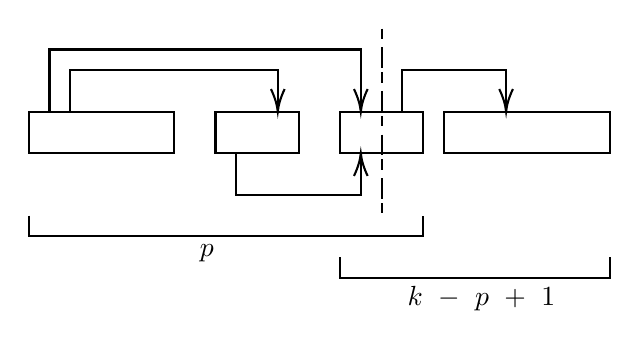
\begin{tikzpicture}[x=0.75pt,y=0.75pt,yscale=-1,xscale=1]
			%uncomment if require: \path (0,300); %set diagram left start at 0, and has height of 300

			%Shape: Rectangle [id:dp5751448069992374] 
			\draw   (100,130) -- (170,130) -- (170,150) -- (100,150) -- cycle ;
			%Shape: Rectangle [id:dp8956649728081978] 
			\draw   (190,130) -- (230,130) -- (230,150) -- (190,150) -- cycle ;
			%Shape: Rectangle [id:dp8836798951210239] 
			\draw   (250,130) -- (290,130) -- (290,150) -- (250,150) -- cycle ;
			%Shape: Rectangle [id:dp07169651712981018] 
			\draw   (300,130) -- (380,130) -- (380,150) -- (300,150) -- cycle ;
			%Straight Lines [id:da8396678932783305] 
			\draw    (110,130) -- (110,100) -- (260,100) -- (260,128) ;
			\draw [shift={(260,130)}, rotate = 270] [color={rgb, 255:red, 0; green, 0; blue, 0 }  ][line width=0.75]    (10.93,-3.29) .. controls (6.95,-1.4) and (3.31,-0.3) .. (0,0) .. controls (3.31,0.3) and (6.95,1.4) .. (10.93,3.29)   ;
			%Straight Lines [id:da8376287767119306] 
			\draw    (120,130) -- (120,110) -- (220,110) -- (220,128) ;
			\draw [shift={(220,130)}, rotate = 270] [color={rgb, 255:red, 0; green, 0; blue, 0 }  ][line width=0.75]    (10.93,-3.29) .. controls (6.95,-1.4) and (3.31,-0.3) .. (0,0) .. controls (3.31,0.3) and (6.95,1.4) .. (10.93,3.29)   ;
			%Straight Lines [id:da7343053938900628] 
			\draw    (200,150) -- (200,170) -- (260,170) -- (260,152) ;
			\draw [shift={(260,150)}, rotate = 90] [color={rgb, 255:red, 0; green, 0; blue, 0 }  ][line width=0.75]    (10.93,-3.29) .. controls (6.95,-1.4) and (3.31,-0.3) .. (0,0) .. controls (3.31,0.3) and (6.95,1.4) .. (10.93,3.29)   ;
			%Straight Lines [id:da02843704523195245] 
			\draw    (280,130) -- (280,110) -- (330,110) -- (330,128) ;
			\draw [shift={(330,130)}, rotate = 270] [color={rgb, 255:red, 0; green, 0; blue, 0 }  ][line width=0.75]    (10.93,-3.29) .. controls (6.95,-1.4) and (3.31,-0.3) .. (0,0) .. controls (3.31,0.3) and (6.95,1.4) .. (10.93,3.29)   ;
			%Straight Lines [id:da4532725638041315] 
			\draw  [dash pattern={on 3.75pt off 3pt on 7.5pt off 1.5pt}]  (270,90) -- (270,180) ;
			%Straight Lines [id:da17944476616348748] 
			\draw    (100,180) -- (100,190) -- (290,190) -- (290,180) ;
			%Straight Lines [id:da1753890360224526] 
			\draw    (250,200) -- (250,210) -- (380,210) -- (380,200) ;

			% Text Node
			\draw (181,192.4) node [anchor=north west][inner sep=0.75pt]    {$p$};
			% Text Node
			\draw (281,212.4) node [anchor=north west][inner sep=0.75pt]    {$k\ -\ p\ +\ 1$};
		\end{tikzpicture}
		\subcaption{Caso $1$.}
	\end{subfigure}
	\hfill
	\begin{subfigure}{0.45\textwidth}

		\tikzset{
			pattern size/.store in=\mcSize,
			pattern size = 5pt,
			pattern thickness/.store in=\mcThickness,
			pattern thickness = 0.3pt,
			pattern radius/.store in=\mcRadius,
			pattern radius = 1pt}
		\makeatletter
		\pgfutil@ifundefined{pgf@pattern@name@_y43ms7xnt}{
			\pgfdeclarepatternformonly[\mcThickness,\mcSize]{_y43ms7xnt}
			{\pgfqpoint{0pt}{-\mcThickness}}
			{\pgfpoint{\mcSize}{\mcSize}}
			{\pgfpoint{\mcSize}{\mcSize}}
			{
				\pgfsetcolor{\tikz@pattern@color}
				\pgfsetlinewidth{\mcThickness}
				\pgfpathmoveto{\pgfqpoint{0pt}{\mcSize}}
				\pgfpathlineto{\pgfpoint{\mcSize+\mcThickness}{-\mcThickness}}
				\pgfusepath{stroke}
			}}
		\makeatother

		% Pattern Info

		\tikzset{
			pattern size/.store in=\mcSize,
			pattern size = 5pt,
			pattern thickness/.store in=\mcThickness,
			pattern thickness = 0.3pt,
			pattern radius/.store in=\mcRadius,
			pattern radius = 1pt}
		\makeatletter
		\pgfutil@ifundefined{pgf@pattern@name@_mifsyi5bu}{
			\pgfdeclarepatternformonly[\mcThickness,\mcSize]{_mifsyi5bu}
			{\pgfqpoint{0pt}{0pt}}
			{\pgfpoint{\mcSize+\mcThickness}{\mcSize+\mcThickness}}
			{\pgfpoint{\mcSize}{\mcSize}}
			{
				\pgfsetcolor{\tikz@pattern@color}
				\pgfsetlinewidth{\mcThickness}
				\pgfpathmoveto{\pgfqpoint{0pt}{0pt}}
				\pgfpathlineto{\pgfpoint{\mcSize+\mcThickness}{\mcSize+\mcThickness}}
				\pgfusepath{stroke}
			}}
		\makeatother
		\tikzset{every picture/.style={line width=0.75pt}} %set default line width to 0.75pt        

		\begin{tikzpicture}[x=0.75pt,y=0.75pt,yscale=-1,xscale=1]
			%uncomment if require: \path (0,300); %set diagram left start at 0, and has height of 300

			%Shape: Rectangle [id:dp5339690558371227] 
			\draw   (120,150) -- (190,150) -- (190,170) -- (120,170) -- cycle ;
			%Straight Lines [id:da850734740747954] 
			\draw    (140,150) -- (140,120) -- (280,120) -- (280,148) ;
			\draw [shift={(280,150)}, rotate = 270] [color={rgb, 255:red, 0; green, 0; blue, 0 }  ][line width=0.75]    (10.93,-3.29) .. controls (6.95,-1.4) and (3.31,-0.3) .. (0,0) .. controls (3.31,0.3) and (6.95,1.4) .. (10.93,3.29)   ;
			%Straight Lines [id:da9735874841202442] 
			\draw    (150,150) -- (150,130) -- (240,130) -- (240,148) ;
			\draw [shift={(240,150)}, rotate = 270] [color={rgb, 255:red, 0; green, 0; blue, 0 }  ][line width=0.75]    (10.93,-3.29) .. controls (6.95,-1.4) and (3.31,-0.3) .. (0,0) .. controls (3.31,0.3) and (6.95,1.4) .. (10.93,3.29)   ;
			%Straight Lines [id:da863983070784418] 
			\draw    (220,170) -- (220,190) -- (280,190) -- (280,172) ;
			\draw [shift={(280,170)}, rotate = 90] [color={rgb, 255:red, 0; green, 0; blue, 0 }  ][line width=0.75]    (10.93,-3.29) .. controls (6.95,-1.4) and (3.31,-0.3) .. (0,0) .. controls (3.31,0.3) and (6.95,1.4) .. (10.93,3.29)   ;
			%Straight Lines [id:da6442133803721162] 
			\draw    (300,150) -- (300,130) -- (350,130) -- (350,148) ;
			\draw [shift={(350,150)}, rotate = 270] [color={rgb, 255:red, 0; green, 0; blue, 0 }  ][line width=0.75]    (10.93,-3.29) .. controls (6.95,-1.4) and (3.31,-0.3) .. (0,0) .. controls (3.31,0.3) and (6.95,1.4) .. (10.93,3.29)   ;
			%Shape: Rectangle [id:dp881091443202814] 
			\draw   (190,150) -- (260,150) -- (260,170) -- (190,170) -- cycle ;
			%Shape: Rectangle [id:dp2693088037465775] 
			\draw   (260,150) -- (330,150) -- (330,170) -- (260,170) -- cycle ;
			%Shape: Rectangle [id:dp6243374270107382] 
			\draw   (330,150) -- (400,150) -- (400,170) -- (330,170) -- cycle ;
			%Straight Lines [id:da11664171795224454] 
			\draw    (150,170) -- (150,190) -- (210,190) -- (210,172) ;
			\draw [shift={(210,170)}, rotate = 90] [color={rgb, 255:red, 0; green, 0; blue, 0 }  ][line width=0.75]    (10.93,-3.29) .. controls (6.95,-1.4) and (3.31,-0.3) .. (0,0) .. controls (3.31,0.3) and (6.95,1.4) .. (10.93,3.29)   ;
			%Straight Lines [id:da43843554948583285] 
			\draw    (130,150) -- (130,140.71) -- (130,110) -- (390,110) -- (390,148) ;
			\draw [shift={(390,150)}, rotate = 270] [color={rgb, 255:red, 0; green, 0; blue, 0 }  ][line width=0.75]    (10.93,-3.29) .. controls (6.95,-1.4) and (3.31,-0.3) .. (0,0) .. controls (3.31,0.3) and (6.95,1.4) .. (10.93,3.29)   ;
			%Shape: Rectangle [id:dp45540530016238834] 
			\draw  [pattern=_y43ms7xnt,pattern size=2.0999999999999996pt,pattern thickness=0.75pt,pattern radius=0pt, pattern color={rgb, 255:red, 0; green, 0; blue, 0}][dash pattern={on 0.84pt off 2.51pt}] (130,150) -- (120,150) -- (120,170) -- (130,170) -- cycle ;
			%Shape: Rectangle [id:dp21031590903119124] 
			\draw  [pattern=_mifsyi5bu,pattern size=2.0999999999999996pt,pattern thickness=0.75pt,pattern radius=0pt, pattern color={rgb, 255:red, 0; green, 0; blue, 0}][dash pattern={on 0.84pt off 2.51pt}] (400,150) -- (390,150) -- (390,170) -- (400,170) -- cycle ;
		\end{tikzpicture}

		\subcaption{Caso $2$.}
	\end{subfigure}
	\caption{Dimostrazione induttiva del numero di pioniere in una parola ben parentesizzata.}
	\label{fig:proof_pioneers}
\end{figure}

Quindi, lo spazio occupato da queste strutture è:
$$
	\begin{aligned}
		 & w          &  & n                                                                                          \\
		 & p          &  & n + o(n) \text{ (sarà necessario introdurre la struttura di rango)}                        \\
		 & \mathbf{E} &  & k  \log_2(n)                                                                               \\
		 & \mathbf{O} &  & k  \log_2(n)                                                                               \\
		 & \mathbf{M} &  & \text{pioniere} \cdot \log_2(n) < 2(2k - 3) \log_2(n) = (4k - 6) \log_2(n) \le 4k\log_2(n)
	\end{aligned}
$$
Sommando, lo spazio occupato è $D_n = 2n + o(n) + 6k \log_2(n) = 2n + 6n + o(n) = 8n + o(n)$ bit.

\subsubsection{Implementazione}
Per implementare la funzione $\mathbf{find\_close}$ che, trovata una parentesi aperta in posizione $p$, restituisce
la posizione in cui si chiude, si deve:
\begin{enumerate}
	\item calcolare gli eccessi di tutte le posizioni del blocco al quale appartiene $p$ con $E$ (tempo logaritmico);
	\item se $p$ è vicina, ossia esiste un'altra posizione nel blocco con lo stesso eccesso,
	      la funzione è completa. Altrimenti, $p$ è la posizione di una parentesi lontana e
	      $j = \mathbf{rank_p}(p)$ è l'indice della pioniera che precede $p$; si può usare $M[j] = p'$ per
	      calcolare la posizione in cui si chiude la pioniera che precede $p$, che diciamo essere in un
	      blocco $b$. Scorrendo indietro, per trovare la chiusa corrispondente, basta trovare la
	      posizione con eccesso uguale all'eccesso di $p$.
\end{enumerate}

Tutto questo richiede tempo $\log_2(n)$ e analogamente per l'implementazione di $\mathbf{find\_open}$.
Per l'implementazione di $\mathbf{enclosed}$, che cerca la prima parentesi aperta che racchiude la parentesi
in posizione $p$, ipotizziamo di aver già trovato la corrispondente $\bar{p}$ con una find e ammettiamo che
l'eccesso di entrambe sia $e$. Inizialmente, si cerca alla sinistra della posizione della parentesi aperta
se c'è una posizione con eccesso $e-1$, che segna l'aperta precedente. Se, nel blocco al quale appartiene
l'aperta, tutte le posizioni hanno eccesso $\ge e-1$, si cerca per una chiusa di eccesso $e-1$ nella parte
a destra del blocco in cui giace la chiusa. Se anche in questo caso non si trova, significa che la parentesi
che si cerca è di eccesso $e-1$ che giace nel blocco a sinistra a quello della parentesi aperta, che ha
come valore di eccesso minore di tale blocco. In tal caso, basta usare il vettore $\mathbf{O}$ per trovare
la posizione della parentesi cercata.

\subsection{Lower bound per parentesi ben bilanciate}
\subsubsection{Foreste ordinate}
Una foresta ordinata è una sequenza ordinata (per numero di nodi) di alberi ordinati (corrispondenti
ad alberi radicati).
\begin{figure}[h]
	\centering
	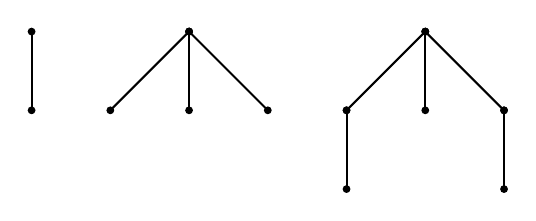
\begin{tikzpicture}
		\draw (0,1)	node[fill,circle, inner sep=1pt] {} -- (0,0) node[fill,circle,inner sep=1pt] {};

		\draw (2,1)	node[fill,circle, inner sep=1pt] {} -- (2,0) node[fill,circle,inner sep=1pt] {};
		\draw (2,1)	node[fill,circle, inner sep=1pt] {} -- (1,0) node[fill,circle,inner sep=1pt] {};
		\draw (2,1)	node[fill,circle, inner sep=1pt] {} -- (3,0) node[fill,circle,inner sep=1pt] {};

		\draw (5,1)	node[fill,circle, inner sep=1pt] {} -- (4,0) node[fill,circle,inner sep=1pt] {};
		\draw (4,0)	node[fill,circle, inner sep=1pt] {} -- (4,-1) node[fill,circle,inner sep=1pt] {};
		\draw (5,1)	node[fill,circle, inner sep=1pt] {} -- (5,0) node[fill,circle,inner sep=1pt] {};
		\draw (5,1)	node[fill,circle, inner sep=1pt] {} -- (6,0) node[fill,circle,inner sep=1pt] {};
		\draw (6,0)	node[fill,circle, inner sep=1pt] {} -- (6,-1) node[fill,circle,inner sep=1pt] {};
	\end{tikzpicture}
	\caption{Foresta ordinata di alberi.}
	\label{fig:ordered_forest}
\end{figure}
Formalmente, definiamo induttivamente una foresta ordinata:
\begin{itemize}
	\item $\langle \rangle$ indica la lista vuota di alberi ed è una foresta ordinata;
	\item se $\langle T_1, \cdots, T_k\rangle$ sono alberi, allora $\langle T_1, \cdots, T_k\rangle$ è una
	      foresta ordinata
	\item se $F$ è una foresta ordinata, $tree(F)$ è un albero radicato in un
	      nuovo nodo che ha come figli tutti gli alberi di $F$.
\end{itemize}

\subsubsection{Isomorfismo tra foreste ordinate e alberi binari}
Definiamo una funzione $\phi$ che associa ad ogni foresta ordinata un preciso albero binario.
Induttivamente,
$$
	\phi(\langle \rangle) = \cdot
$$
ossia $\phi$ di una foresta vuota è un albero costituito da una singola radice.
$$
	\phi(\langle tree(F), T_1, \cdots, T_k>\rangle) = (\phi(F), \phi(\langle T_1, \cdots, T_k\rangle))
$$

\begin{figure}[h]
	\centering
	\tikzset{every picture/.style={line width=0.75pt}} %set default line width to 0.75pt        

	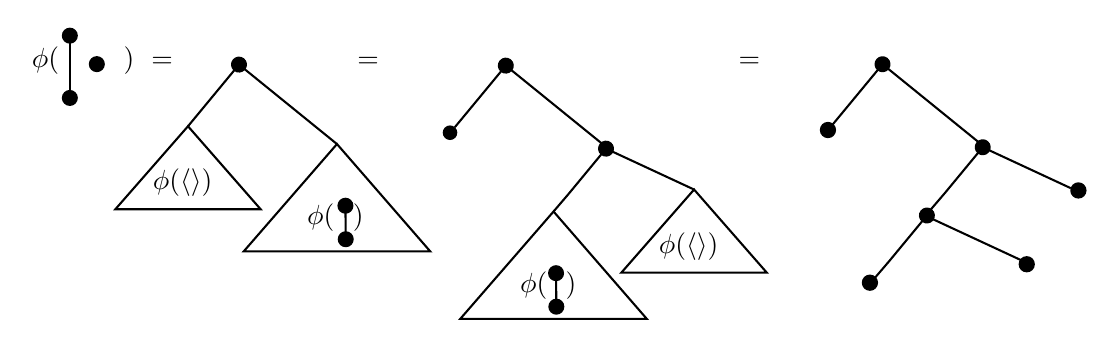
\begin{tikzpicture}[x=0.75pt,y=0.75pt,yscale=-1,xscale=1]
		%uncomment if require: \path (0,300); %set diagram left start at 0, and has height of 300

		%Straight Lines [id:da1467409507063523] 
		\draw    (144.93,41.07) -- (144.93,71.07) ;
		\draw [shift={(144.93,71.07)}, rotate = 90] [color={rgb, 255:red, 0; green, 0; blue, 0 }  ][fill={rgb, 255:red, 0; green, 0; blue, 0 }  ][line width=0.75]      (0, 0) circle [x radius= 3.35, y radius= 3.35]   ;
		\draw [shift={(144.93,41.07)}, rotate = 90] [color={rgb, 255:red, 0; green, 0; blue, 0 }  ][fill={rgb, 255:red, 0; green, 0; blue, 0 }  ][line width=0.75]      (0, 0) circle [x radius= 3.35, y radius= 3.35]   ;
		%Shape: Circle [id:dp48951213847038366] 
		\draw  [fill={rgb, 255:red, 0; green, 0; blue, 0 }  ,fill opacity=1 ] (154.57,54.79) .. controls (154.57,52.93) and (156.07,51.43) .. (157.93,51.43) .. controls (159.78,51.43) and (161.29,52.93) .. (161.29,54.79) .. controls (161.29,56.64) and (159.78,58.14) .. (157.93,58.14) .. controls (156.07,58.14) and (154.57,56.64) .. (154.57,54.79) -- cycle ;

		%Straight Lines [id:da5368285010745462] 
		\draw    (226.43,55) -- (208.31,76.91) -- (201.86,84.71) ;
		\draw [shift={(226.43,55)}, rotate = 129.59] [color={rgb, 255:red, 0; green, 0; blue, 0 }  ][fill={rgb, 255:red, 0; green, 0; blue, 0 }  ][line width=0.75]      (0, 0) circle [x radius= 3.35, y radius= 3.35]   ;
		%Shape: Triangle [id:dp5019688866391238] 
		\draw   (201.86,84.71) -- (236.86,124.71) -- (166.86,124.71) -- cycle ;
		%Shape: Triangle [id:dp12657672899601724] 
		\draw   (273.64,93.29) -- (318.57,145) -- (228.71,145) -- cycle ;
		%Straight Lines [id:da934069022901869] 
		\draw    (226.43,55) -- (273.64,93.29) ;
		%Straight Lines [id:da2898443038516424] 
		\draw    (277.71,123) -- (277.86,139.14) ;
		\draw [shift={(277.86,139.14)}, rotate = 89.49] [color={rgb, 255:red, 0; green, 0; blue, 0 }  ][fill={rgb, 255:red, 0; green, 0; blue, 0 }  ][line width=0.75]      (0, 0) circle [x radius= 3.35, y radius= 3.35]   ;
		\draw [shift={(277.71,123)}, rotate = 89.49] [color={rgb, 255:red, 0; green, 0; blue, 0 }  ][fill={rgb, 255:red, 0; green, 0; blue, 0 }  ][line width=0.75]      (0, 0) circle [x radius= 3.35, y radius= 3.35]   ;
		%Straight Lines [id:da8113066852584067] 
		\draw    (354.98,55.5) -- (336.86,77.41) -- (330.4,85.21) ;
		\draw [shift={(354.98,55.5)}, rotate = 129.59] [color={rgb, 255:red, 0; green, 0; blue, 0 }  ][fill={rgb, 255:red, 0; green, 0; blue, 0 }  ][line width=0.75]      (0, 0) circle [x radius= 3.35, y radius= 3.35]   ;
		%Straight Lines [id:da7241289121021388] 
		\draw    (354.98,55.5) -- (402.19,93.79) ;
		%Shape: Circle [id:dp6494084453696087] 
		\draw  [fill={rgb, 255:red, 0; green, 0; blue, 0 }  ,fill opacity=1 ] (325.1,87.83) .. controls (325.1,86.18) and (326.44,84.83) .. (328.1,84.83) .. controls (329.76,84.83) and (331.1,86.18) .. (331.1,87.83) .. controls (331.1,89.49) and (329.76,90.83) .. (328.1,90.83) .. controls (326.44,90.83) and (325.1,89.49) .. (325.1,87.83) -- cycle ;
		%Straight Lines [id:da4037066529287967] 
		\draw    (403.26,95.5) -- (385.15,117.41) -- (377.98,125.79) ;
		\draw [shift={(403.26,95.5)}, rotate = 129.59] [color={rgb, 255:red, 0; green, 0; blue, 0 }  ][fill={rgb, 255:red, 0; green, 0; blue, 0 }  ][line width=0.75]      (0, 0) circle [x radius= 3.35, y radius= 3.35]   ;
		%Shape: Triangle [id:dp04881880314765141] 
		\draw   (445.69,115.21) -- (480.69,155.21) -- (410.69,155.21) -- cycle ;

		%Shape: Triangle [id:dp12559883893437063] 
		\draw   (377.98,125.79) -- (422.9,177.5) -- (333.05,177.5) -- cycle ;
		%Straight Lines [id:da48087885685526743] 
		\draw    (379.19,155.5) -- (379.33,171.64) ;
		\draw [shift={(379.33,171.64)}, rotate = 89.49] [color={rgb, 255:red, 0; green, 0; blue, 0 }  ][fill={rgb, 255:red, 0; green, 0; blue, 0 }  ][line width=0.75]      (0, 0) circle [x radius= 3.35, y radius= 3.35]   ;
		\draw [shift={(379.19,155.5)}, rotate = 89.49] [color={rgb, 255:red, 0; green, 0; blue, 0 }  ][fill={rgb, 255:red, 0; green, 0; blue, 0 }  ][line width=0.75]      (0, 0) circle [x radius= 3.35, y radius= 3.35]   ;
		%Straight Lines [id:da02388870469608051] 
		\draw    (403.26,95.5) -- (445.69,115.21) ;
		%Straight Lines [id:da6273665141516217] 
		\draw    (536.48,54.83) -- (518.36,76.74) -- (511.9,84.55) ;
		\draw [shift={(536.48,54.83)}, rotate = 129.59] [color={rgb, 255:red, 0; green, 0; blue, 0 }  ][fill={rgb, 255:red, 0; green, 0; blue, 0 }  ][line width=0.75]      (0, 0) circle [x radius= 3.35, y radius= 3.35]   ;
		%Straight Lines [id:da5905284436508569] 
		\draw    (536.48,54.83) -- (583.69,93.12) ;
		%Straight Lines [id:da2030740854922638] 
		\draw    (584.76,94.83) -- (566.65,116.74) -- (559.48,125.12) ;
		\draw [shift={(584.76,94.83)}, rotate = 129.59] [color={rgb, 255:red, 0; green, 0; blue, 0 }  ][fill={rgb, 255:red, 0; green, 0; blue, 0 }  ][line width=0.75]      (0, 0) circle [x radius= 3.35, y radius= 3.35]   ;
		%Straight Lines [id:da49066689108397754] 
		\draw    (584.76,94.83) -- (627.19,114.55) ;
		%Straight Lines [id:da38720603069737713] 
		\draw    (557.87,127.72) -- (539.76,149.63) -- (532.59,158.01) ;
		\draw [shift={(557.87,127.72)}, rotate = 129.59] [color={rgb, 255:red, 0; green, 0; blue, 0 }  ][fill={rgb, 255:red, 0; green, 0; blue, 0 }  ][line width=0.75]      (0, 0) circle [x radius= 3.35, y radius= 3.35]   ;
		%Straight Lines [id:da1048947282900694] 
		\draw    (560.76,129.5) -- (603.19,149.21) ;
		%Shape: Circle [id:dp32417892244375524] 
		\draw  [fill={rgb, 255:red, 0; green, 0; blue, 0 }  ,fill opacity=1 ] (533.82,160.09) .. controls (533.82,158.2) and (532.3,156.67) .. (530.41,156.67) .. controls (528.53,156.67) and (527,158.2) .. (527,160.09) .. controls (527,161.97) and (528.53,163.5) .. (530.41,163.5) .. controls (532.3,163.5) and (533.82,161.97) .. (533.82,160.09) -- cycle ;
		%Shape: Circle [id:dp9675952466326133] 
		\draw  [fill={rgb, 255:red, 0; green, 0; blue, 0 }  ,fill opacity=1 ] (513.6,86.53) .. controls (513.6,84.65) and (512.07,83.12) .. (510.19,83.12) .. controls (508.3,83.12) and (506.78,84.65) .. (506.78,86.53) .. controls (506.78,88.42) and (508.3,89.94) .. (510.19,89.94) .. controls (512.07,89.94) and (513.6,88.42) .. (513.6,86.53) -- cycle ;

		%Shape: Circle [id:dp5658104800173653] 
		\draw  [fill={rgb, 255:red, 0; green, 0; blue, 0 }  ,fill opacity=1 ] (609.38,151.2) .. controls (609.38,149.31) and (607.85,147.79) .. (605.97,147.79) .. controls (604.08,147.79) and (602.55,149.31) .. (602.55,151.2) .. controls (602.55,153.08) and (604.08,154.61) .. (605.97,154.61) .. controls (607.85,154.61) and (609.38,153.08) .. (609.38,151.2) -- cycle ;
		%Shape: Circle [id:dp12193907009892957] 
		\draw  [fill={rgb, 255:red, 0; green, 0; blue, 0 }  ,fill opacity=1 ] (634.27,115.64) .. controls (634.27,113.76) and (632.74,112.23) .. (630.86,112.23) .. controls (628.97,112.23) and (627.44,113.76) .. (627.44,115.64) .. controls (627.44,117.53) and (628.97,119.06) .. (630.86,119.06) .. controls (632.74,119.06) and (634.27,117.53) .. (634.27,115.64) -- cycle ;


		% Text Node
		\draw (125.12,44.91) node [anchor=north west][inner sep=0.75pt]    {$\phi ( \ \ \ \ \ \ \ ) \ =\ \ \ \ \ \ \ \ \ \ \ \ \ \ \ \ \ \ \ \ =\ \ \ \ \ \ \ \ \ \ \ \ \ \ \ \ \ \ \ \ \ \ \ \ \ \ \ \ \ \ \ \ \ \ \ \ \ \ \ =\ $};
		% Text Node
		\draw (427.26,134.33) node [anchor=north west][inner sep=0.75pt]    {$\phi ( \langle \rangle )$};
		% Text Node
		\draw (183.43,103.83) node [anchor=north west][inner sep=0.75pt]    {$\phi ( \langle \rangle )$};
		% Text Node
		\draw (257.75,120.69) node [anchor=north west][inner sep=0.75pt]    {$\phi ( \ \ )$};
		% Text Node
		\draw (360.33,153.19) node [anchor=north west][inner sep=0.75pt]    {$\phi ( \ \ )$};


	\end{tikzpicture}
	\caption{Esempio di calcolo isomorfismo tra foreste e alberi binari.}
	\label{fig:iso_forest_bintree_example}
\end{figure}



\begin{figure}[h]
	\centering



	\tikzset{every picture/.style={line width=0.75pt}} %set default line width to 0.75pt        

	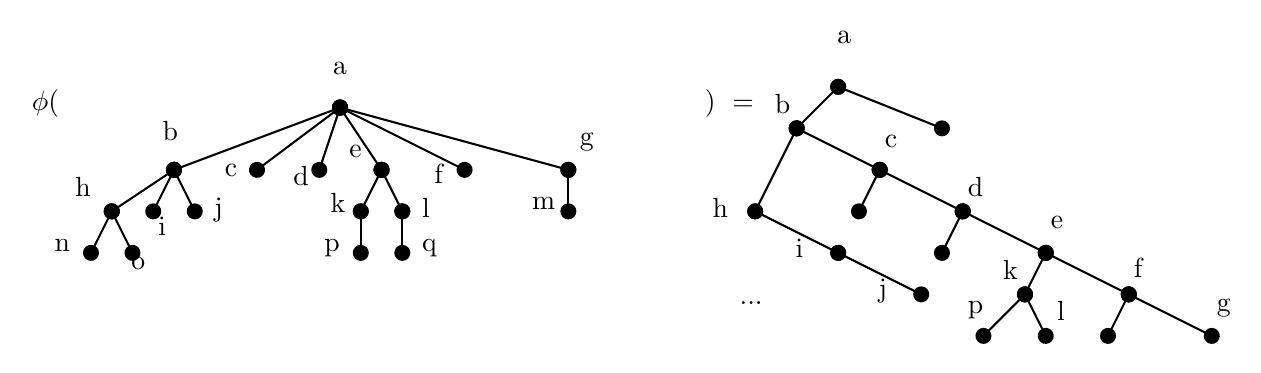
\begin{tikzpicture}[x=0.75pt,y=0.75pt,yscale=-1,xscale=1]
		%uncomment if require: \path (0,300); %set diagram left start at 0, and has height of 300

		%Straight Lines [id:da7390170116429094] 
		\draw    (220,90) -- (330,120) ;
		\draw [shift={(330,120)}, rotate = 15.26] [color={rgb, 255:red, 0; green, 0; blue, 0 }  ][fill={rgb, 255:red, 0; green, 0; blue, 0 }  ][line width=0.75]      (0, 0) circle [x radius= 3.35, y radius= 3.35]   ;
		\draw [shift={(220,90)}, rotate = 15.26] [color={rgb, 255:red, 0; green, 0; blue, 0 }  ][fill={rgb, 255:red, 0; green, 0; blue, 0 }  ][line width=0.75]      (0, 0) circle [x radius= 3.35, y radius= 3.35]   ;
		%Straight Lines [id:da039244879101243746] 
		\draw    (220,90) -- (280,120) ;
		\draw [shift={(280,120)}, rotate = 26.57] [color={rgb, 255:red, 0; green, 0; blue, 0 }  ][fill={rgb, 255:red, 0; green, 0; blue, 0 }  ][line width=0.75]      (0, 0) circle [x radius= 3.35, y radius= 3.35]   ;
		\draw [shift={(220,90)}, rotate = 26.57] [color={rgb, 255:red, 0; green, 0; blue, 0 }  ][fill={rgb, 255:red, 0; green, 0; blue, 0 }  ][line width=0.75]      (0, 0) circle [x radius= 3.35, y radius= 3.35]   ;
		%Straight Lines [id:da9807403722275164] 
		\draw    (220,90) -- (240,120) ;
		\draw [shift={(240,120)}, rotate = 56.31] [color={rgb, 255:red, 0; green, 0; blue, 0 }  ][fill={rgb, 255:red, 0; green, 0; blue, 0 }  ][line width=0.75]      (0, 0) circle [x radius= 3.35, y radius= 3.35]   ;
		\draw [shift={(220,90)}, rotate = 56.31] [color={rgb, 255:red, 0; green, 0; blue, 0 }  ][fill={rgb, 255:red, 0; green, 0; blue, 0 }  ][line width=0.75]      (0, 0) circle [x radius= 3.35, y radius= 3.35]   ;
		%Straight Lines [id:da03267007977703551] 
		\draw    (220,90) -- (210,120) ;
		\draw [shift={(210,120)}, rotate = 108.43] [color={rgb, 255:red, 0; green, 0; blue, 0 }  ][fill={rgb, 255:red, 0; green, 0; blue, 0 }  ][line width=0.75]      (0, 0) circle [x radius= 3.35, y radius= 3.35]   ;
		\draw [shift={(220,90)}, rotate = 108.43] [color={rgb, 255:red, 0; green, 0; blue, 0 }  ][fill={rgb, 255:red, 0; green, 0; blue, 0 }  ][line width=0.75]      (0, 0) circle [x radius= 3.35, y radius= 3.35]   ;
		%Straight Lines [id:da3117293837981189] 
		\draw    (220,90) -- (140,120) ;
		\draw [shift={(140,120)}, rotate = 159.44] [color={rgb, 255:red, 0; green, 0; blue, 0 }  ][fill={rgb, 255:red, 0; green, 0; blue, 0 }  ][line width=0.75]      (0, 0) circle [x radius= 3.35, y radius= 3.35]   ;
		\draw [shift={(220,90)}, rotate = 159.44] [color={rgb, 255:red, 0; green, 0; blue, 0 }  ][fill={rgb, 255:red, 0; green, 0; blue, 0 }  ][line width=0.75]      (0, 0) circle [x radius= 3.35, y radius= 3.35]   ;
		%Straight Lines [id:da5543598400532516] 
		\draw    (220,90) -- (180,120) ;
		\draw [shift={(180,120)}, rotate = 143.13] [color={rgb, 255:red, 0; green, 0; blue, 0 }  ][fill={rgb, 255:red, 0; green, 0; blue, 0 }  ][line width=0.75]      (0, 0) circle [x radius= 3.35, y radius= 3.35]   ;
		\draw [shift={(220,90)}, rotate = 143.13] [color={rgb, 255:red, 0; green, 0; blue, 0 }  ][fill={rgb, 255:red, 0; green, 0; blue, 0 }  ][line width=0.75]      (0, 0) circle [x radius= 3.35, y radius= 3.35]   ;
		%Straight Lines [id:da6616928412892461] 
		\draw    (140,120) -- (130,140) ;
		\draw [shift={(130,140)}, rotate = 116.57] [color={rgb, 255:red, 0; green, 0; blue, 0 }  ][fill={rgb, 255:red, 0; green, 0; blue, 0 }  ][line width=0.75]      (0, 0) circle [x radius= 3.35, y radius= 3.35]   ;
		\draw [shift={(140,120)}, rotate = 116.57] [color={rgb, 255:red, 0; green, 0; blue, 0 }  ][fill={rgb, 255:red, 0; green, 0; blue, 0 }  ][line width=0.75]      (0, 0) circle [x radius= 3.35, y radius= 3.35]   ;
		%Straight Lines [id:da5001878304038733] 
		\draw    (140,120) -- (110,140) ;
		\draw [shift={(110,140)}, rotate = 146.31] [color={rgb, 255:red, 0; green, 0; blue, 0 }  ][fill={rgb, 255:red, 0; green, 0; blue, 0 }  ][line width=0.75]      (0, 0) circle [x radius= 3.35, y radius= 3.35]   ;
		\draw [shift={(140,120)}, rotate = 146.31] [color={rgb, 255:red, 0; green, 0; blue, 0 }  ][fill={rgb, 255:red, 0; green, 0; blue, 0 }  ][line width=0.75]      (0, 0) circle [x radius= 3.35, y radius= 3.35]   ;
		%Straight Lines [id:da35297443192918876] 
		\draw    (140,120) -- (150,140) ;
		\draw [shift={(150,140)}, rotate = 63.43] [color={rgb, 255:red, 0; green, 0; blue, 0 }  ][fill={rgb, 255:red, 0; green, 0; blue, 0 }  ][line width=0.75]      (0, 0) circle [x radius= 3.35, y radius= 3.35]   ;
		\draw [shift={(140,120)}, rotate = 63.43] [color={rgb, 255:red, 0; green, 0; blue, 0 }  ][fill={rgb, 255:red, 0; green, 0; blue, 0 }  ][line width=0.75]      (0, 0) circle [x radius= 3.35, y radius= 3.35]   ;
		%Straight Lines [id:da30077845664351066] 
		\draw    (110,140) -- (100,160) ;
		\draw [shift={(100,160)}, rotate = 116.57] [color={rgb, 255:red, 0; green, 0; blue, 0 }  ][fill={rgb, 255:red, 0; green, 0; blue, 0 }  ][line width=0.75]      (0, 0) circle [x radius= 3.35, y radius= 3.35]   ;
		\draw [shift={(110,140)}, rotate = 116.57] [color={rgb, 255:red, 0; green, 0; blue, 0 }  ][fill={rgb, 255:red, 0; green, 0; blue, 0 }  ][line width=0.75]      (0, 0) circle [x radius= 3.35, y radius= 3.35]   ;
		%Straight Lines [id:da5436015840206943] 
		\draw    (110,140) -- (120,160) ;
		\draw [shift={(120,160)}, rotate = 63.43] [color={rgb, 255:red, 0; green, 0; blue, 0 }  ][fill={rgb, 255:red, 0; green, 0; blue, 0 }  ][line width=0.75]      (0, 0) circle [x radius= 3.35, y radius= 3.35]   ;
		\draw [shift={(110,140)}, rotate = 63.43] [color={rgb, 255:red, 0; green, 0; blue, 0 }  ][fill={rgb, 255:red, 0; green, 0; blue, 0 }  ][line width=0.75]      (0, 0) circle [x radius= 3.35, y radius= 3.35]   ;
		%Straight Lines [id:da3418649793206039] 
		\draw    (240,120) -- (230,140) ;
		\draw [shift={(230,140)}, rotate = 116.57] [color={rgb, 255:red, 0; green, 0; blue, 0 }  ][fill={rgb, 255:red, 0; green, 0; blue, 0 }  ][line width=0.75]      (0, 0) circle [x radius= 3.35, y radius= 3.35]   ;
		\draw [shift={(240,120)}, rotate = 116.57] [color={rgb, 255:red, 0; green, 0; blue, 0 }  ][fill={rgb, 255:red, 0; green, 0; blue, 0 }  ][line width=0.75]      (0, 0) circle [x radius= 3.35, y radius= 3.35]   ;
		%Straight Lines [id:da5537357380053466] 
		\draw    (240,120) -- (250,140) ;
		\draw [shift={(250,140)}, rotate = 63.43] [color={rgb, 255:red, 0; green, 0; blue, 0 }  ][fill={rgb, 255:red, 0; green, 0; blue, 0 }  ][line width=0.75]      (0, 0) circle [x radius= 3.35, y radius= 3.35]   ;
		\draw [shift={(240,120)}, rotate = 63.43] [color={rgb, 255:red, 0; green, 0; blue, 0 }  ][fill={rgb, 255:red, 0; green, 0; blue, 0 }  ][line width=0.75]      (0, 0) circle [x radius= 3.35, y radius= 3.35]   ;
		%Straight Lines [id:da596511628614987] 
		\draw    (330,120) -- (330,140) ;
		\draw [shift={(330,140)}, rotate = 90] [color={rgb, 255:red, 0; green, 0; blue, 0 }  ][fill={rgb, 255:red, 0; green, 0; blue, 0 }  ][line width=0.75]      (0, 0) circle [x radius= 3.35, y radius= 3.35]   ;
		\draw [shift={(330,120)}, rotate = 90] [color={rgb, 255:red, 0; green, 0; blue, 0 }  ][fill={rgb, 255:red, 0; green, 0; blue, 0 }  ][line width=0.75]      (0, 0) circle [x radius= 3.35, y radius= 3.35]   ;
		%Straight Lines [id:da9692313360351018] 
		\draw    (250,140) -- (250,160) ;
		\draw [shift={(250,160)}, rotate = 90] [color={rgb, 255:red, 0; green, 0; blue, 0 }  ][fill={rgb, 255:red, 0; green, 0; blue, 0 }  ][line width=0.75]      (0, 0) circle [x radius= 3.35, y radius= 3.35]   ;
		\draw [shift={(250,140)}, rotate = 90] [color={rgb, 255:red, 0; green, 0; blue, 0 }  ][fill={rgb, 255:red, 0; green, 0; blue, 0 }  ][line width=0.75]      (0, 0) circle [x radius= 3.35, y radius= 3.35]   ;
		%Straight Lines [id:da3464424144057545] 
		\draw    (230,140) -- (230,160) ;
		\draw [shift={(230,160)}, rotate = 90] [color={rgb, 255:red, 0; green, 0; blue, 0 }  ][fill={rgb, 255:red, 0; green, 0; blue, 0 }  ][line width=0.75]      (0, 0) circle [x radius= 3.35, y radius= 3.35]   ;
		\draw [shift={(230,140)}, rotate = 90] [color={rgb, 255:red, 0; green, 0; blue, 0 }  ][fill={rgb, 255:red, 0; green, 0; blue, 0 }  ][line width=0.75]      (0, 0) circle [x radius= 3.35, y radius= 3.35]   ;
		%Straight Lines [id:da9449001958581409] 
		\draw    (460,80) -- (510,100) ;
		\draw [shift={(510,100)}, rotate = 21.8] [color={rgb, 255:red, 0; green, 0; blue, 0 }  ][fill={rgb, 255:red, 0; green, 0; blue, 0 }  ][line width=0.75]      (0, 0) circle [x radius= 3.35, y radius= 3.35]   ;
		\draw [shift={(460,80)}, rotate = 21.8] [color={rgb, 255:red, 0; green, 0; blue, 0 }  ][fill={rgb, 255:red, 0; green, 0; blue, 0 }  ][line width=0.75]      (0, 0) circle [x radius= 3.35, y radius= 3.35]   ;
		%Straight Lines [id:da5101057369964663] 
		\draw    (460,80) -- (440,100) ;
		\draw [shift={(440,100)}, rotate = 135] [color={rgb, 255:red, 0; green, 0; blue, 0 }  ][fill={rgb, 255:red, 0; green, 0; blue, 0 }  ][line width=0.75]      (0, 0) circle [x radius= 3.35, y radius= 3.35]   ;
		\draw [shift={(460,80)}, rotate = 135] [color={rgb, 255:red, 0; green, 0; blue, 0 }  ][fill={rgb, 255:red, 0; green, 0; blue, 0 }  ][line width=0.75]      (0, 0) circle [x radius= 3.35, y radius= 3.35]   ;
		%Straight Lines [id:da7168760346038819] 
		\draw    (440,100) -- (480,120) ;
		\draw [shift={(480,120)}, rotate = 26.57] [color={rgb, 255:red, 0; green, 0; blue, 0 }  ][fill={rgb, 255:red, 0; green, 0; blue, 0 }  ][line width=0.75]      (0, 0) circle [x radius= 3.35, y radius= 3.35]   ;
		\draw [shift={(440,100)}, rotate = 26.57] [color={rgb, 255:red, 0; green, 0; blue, 0 }  ][fill={rgb, 255:red, 0; green, 0; blue, 0 }  ][line width=0.75]      (0, 0) circle [x radius= 3.35, y radius= 3.35]   ;
		%Straight Lines [id:da7536172846092781] 
		\draw    (480,120) -- (520,140) ;
		\draw [shift={(520,140)}, rotate = 26.57] [color={rgb, 255:red, 0; green, 0; blue, 0 }  ][fill={rgb, 255:red, 0; green, 0; blue, 0 }  ][line width=0.75]      (0, 0) circle [x radius= 3.35, y radius= 3.35]   ;
		\draw [shift={(480,120)}, rotate = 26.57] [color={rgb, 255:red, 0; green, 0; blue, 0 }  ][fill={rgb, 255:red, 0; green, 0; blue, 0 }  ][line width=0.75]      (0, 0) circle [x radius= 3.35, y radius= 3.35]   ;
		%Straight Lines [id:da06546573584424464] 
		\draw    (520,140) -- (560,160) ;
		\draw [shift={(560,160)}, rotate = 26.57] [color={rgb, 255:red, 0; green, 0; blue, 0 }  ][fill={rgb, 255:red, 0; green, 0; blue, 0 }  ][line width=0.75]      (0, 0) circle [x radius= 3.35, y radius= 3.35]   ;
		\draw [shift={(520,140)}, rotate = 26.57] [color={rgb, 255:red, 0; green, 0; blue, 0 }  ][fill={rgb, 255:red, 0; green, 0; blue, 0 }  ][line width=0.75]      (0, 0) circle [x radius= 3.35, y radius= 3.35]   ;
		%Straight Lines [id:da31121333233660786] 
		\draw    (560,160) -- (600,180) ;
		\draw [shift={(600,180)}, rotate = 26.57] [color={rgb, 255:red, 0; green, 0; blue, 0 }  ][fill={rgb, 255:red, 0; green, 0; blue, 0 }  ][line width=0.75]      (0, 0) circle [x radius= 3.35, y radius= 3.35]   ;
		\draw [shift={(560,160)}, rotate = 26.57] [color={rgb, 255:red, 0; green, 0; blue, 0 }  ][fill={rgb, 255:red, 0; green, 0; blue, 0 }  ][line width=0.75]      (0, 0) circle [x radius= 3.35, y radius= 3.35]   ;
		%Straight Lines [id:da9734645903114482] 
		\draw    (600,180) -- (640,200) ;
		\draw [shift={(640,200)}, rotate = 26.57] [color={rgb, 255:red, 0; green, 0; blue, 0 }  ][fill={rgb, 255:red, 0; green, 0; blue, 0 }  ][line width=0.75]      (0, 0) circle [x radius= 3.35, y radius= 3.35]   ;
		\draw [shift={(600,180)}, rotate = 26.57] [color={rgb, 255:red, 0; green, 0; blue, 0 }  ][fill={rgb, 255:red, 0; green, 0; blue, 0 }  ][line width=0.75]      (0, 0) circle [x radius= 3.35, y radius= 3.35]   ;
		%Straight Lines [id:da3400373607542443] 
		\draw    (480,120) -- (470,140) ;
		\draw [shift={(470,140)}, rotate = 116.57] [color={rgb, 255:red, 0; green, 0; blue, 0 }  ][fill={rgb, 255:red, 0; green, 0; blue, 0 }  ][line width=0.75]      (0, 0) circle [x radius= 3.35, y radius= 3.35]   ;
		\draw [shift={(480,120)}, rotate = 116.57] [color={rgb, 255:red, 0; green, 0; blue, 0 }  ][fill={rgb, 255:red, 0; green, 0; blue, 0 }  ][line width=0.75]      (0, 0) circle [x radius= 3.35, y radius= 3.35]   ;
		%Straight Lines [id:da8071946852447195] 
		\draw    (520,140) -- (510,160) ;
		\draw [shift={(510,160)}, rotate = 116.57] [color={rgb, 255:red, 0; green, 0; blue, 0 }  ][fill={rgb, 255:red, 0; green, 0; blue, 0 }  ][line width=0.75]      (0, 0) circle [x radius= 3.35, y radius= 3.35]   ;
		\draw [shift={(520,140)}, rotate = 116.57] [color={rgb, 255:red, 0; green, 0; blue, 0 }  ][fill={rgb, 255:red, 0; green, 0; blue, 0 }  ][line width=0.75]      (0, 0) circle [x radius= 3.35, y radius= 3.35]   ;
		%Straight Lines [id:da9920119862914486] 
		\draw    (600,180) -- (590,200) ;
		\draw [shift={(590,200)}, rotate = 116.57] [color={rgb, 255:red, 0; green, 0; blue, 0 }  ][fill={rgb, 255:red, 0; green, 0; blue, 0 }  ][line width=0.75]      (0, 0) circle [x radius= 3.35, y radius= 3.35]   ;
		\draw [shift={(600,180)}, rotate = 116.57] [color={rgb, 255:red, 0; green, 0; blue, 0 }  ][fill={rgb, 255:red, 0; green, 0; blue, 0 }  ][line width=0.75]      (0, 0) circle [x radius= 3.35, y radius= 3.35]   ;
		%Straight Lines [id:da6764843933308277] 
		\draw    (560,160) -- (550,180) ;
		\draw [shift={(550,180)}, rotate = 116.57] [color={rgb, 255:red, 0; green, 0; blue, 0 }  ][fill={rgb, 255:red, 0; green, 0; blue, 0 }  ][line width=0.75]      (0, 0) circle [x radius= 3.35, y radius= 3.35]   ;
		\draw [shift={(560,160)}, rotate = 116.57] [color={rgb, 255:red, 0; green, 0; blue, 0 }  ][fill={rgb, 255:red, 0; green, 0; blue, 0 }  ][line width=0.75]      (0, 0) circle [x radius= 3.35, y radius= 3.35]   ;
		%Straight Lines [id:da9822121216527463] 
		\draw    (550,180) -- (530,200) ;
		\draw [shift={(530,200)}, rotate = 135] [color={rgb, 255:red, 0; green, 0; blue, 0 }  ][fill={rgb, 255:red, 0; green, 0; blue, 0 }  ][line width=0.75]      (0, 0) circle [x radius= 3.35, y radius= 3.35]   ;
		\draw [shift={(550,180)}, rotate = 135] [color={rgb, 255:red, 0; green, 0; blue, 0 }  ][fill={rgb, 255:red, 0; green, 0; blue, 0 }  ][line width=0.75]      (0, 0) circle [x radius= 3.35, y radius= 3.35]   ;
		%Straight Lines [id:da3765788262191845] 
		\draw    (550,180) -- (560,200) ;
		\draw [shift={(560,200)}, rotate = 63.43] [color={rgb, 255:red, 0; green, 0; blue, 0 }  ][fill={rgb, 255:red, 0; green, 0; blue, 0 }  ][line width=0.75]      (0, 0) circle [x radius= 3.35, y radius= 3.35]   ;
		\draw [shift={(550,180)}, rotate = 63.43] [color={rgb, 255:red, 0; green, 0; blue, 0 }  ][fill={rgb, 255:red, 0; green, 0; blue, 0 }  ][line width=0.75]      (0, 0) circle [x radius= 3.35, y radius= 3.35]   ;
		%Straight Lines [id:da057732075656578896] 
		\draw    (420,140) -- (460,160) ;
		\draw [shift={(460,160)}, rotate = 26.57] [color={rgb, 255:red, 0; green, 0; blue, 0 }  ][fill={rgb, 255:red, 0; green, 0; blue, 0 }  ][line width=0.75]      (0, 0) circle [x radius= 3.35, y radius= 3.35]   ;
		\draw [shift={(420,140)}, rotate = 26.57] [color={rgb, 255:red, 0; green, 0; blue, 0 }  ][fill={rgb, 255:red, 0; green, 0; blue, 0 }  ][line width=0.75]      (0, 0) circle [x radius= 3.35, y radius= 3.35]   ;
		%Straight Lines [id:da6702517354459413] 
		\draw    (460,160) -- (500,180) ;
		\draw [shift={(500,180)}, rotate = 26.57] [color={rgb, 255:red, 0; green, 0; blue, 0 }  ][fill={rgb, 255:red, 0; green, 0; blue, 0 }  ][line width=0.75]      (0, 0) circle [x radius= 3.35, y radius= 3.35]   ;
		\draw [shift={(460,160)}, rotate = 26.57] [color={rgb, 255:red, 0; green, 0; blue, 0 }  ][fill={rgb, 255:red, 0; green, 0; blue, 0 }  ][line width=0.75]      (0, 0) circle [x radius= 3.35, y radius= 3.35]   ;
		%Straight Lines [id:da6027456046960759] 
		\draw    (440,100) -- (420,140) ;
		\draw [shift={(420,140)}, rotate = 116.57] [color={rgb, 255:red, 0; green, 0; blue, 0 }  ][fill={rgb, 255:red, 0; green, 0; blue, 0 }  ][line width=0.75]      (0, 0) circle [x radius= 3.35, y radius= 3.35]   ;
		\draw [shift={(440,100)}, rotate = 116.57] [color={rgb, 255:red, 0; green, 0; blue, 0 }  ][fill={rgb, 255:red, 0; green, 0; blue, 0 }  ][line width=0.75]      (0, 0) circle [x radius= 3.35, y radius= 3.35]   ;

		% Text Node
		\draw (70,80) node [anchor=north west][inner sep=0.75pt]    {$\phi ( \ \ \ \ \ \ \ \ \ \ \ \ \ \ \ \ \ \ \ \ \ \ \ \ \ \ \ \ \ \ \ \ \ \ \ \ \ \ \ \ \ \ \ \ \ \ \ \ \ \ \ \ \ \ \ \ \ \ \ \ \ \ \ \ \ \ \ \ \ \ ) \ =\ $};
		% Text Node
		\draw (215,67) node [anchor=north west][inner sep=0.75pt]   [align=left] {a};
		% Text Node
		\draw (133,95) node [anchor=north west][inner sep=0.75pt]   [align=left] {b};
		% Text Node
		\draw (163,116) node [anchor=north west][inner sep=0.75pt]   [align=left] {c};
		% Text Node
		\draw (196,117) node [anchor=north west][inner sep=0.75pt]   [align=left] {d};
		% Text Node
		\draw (223,107) node [anchor=north west][inner sep=0.75pt]   [align=left] {e};
		% Text Node
		\draw (264,116) node [anchor=north west][inner sep=0.75pt]   [align=left] {f};
		% Text Node
		\draw (334,101) node [anchor=north west][inner sep=0.75pt]   [align=left] {g};
		% Text Node
		\draw (91,122) node [anchor=north west][inner sep=0.75pt]   [align=left] {h};
		% Text Node
		\draw (131,141) node [anchor=north west][inner sep=0.75pt]   [align=left] {i};
		% Text Node
		\draw (158,132) node [anchor=north west][inner sep=0.75pt]   [align=left] {j};
		% Text Node
		\draw (214,130) node [anchor=north west][inner sep=0.75pt]   [align=left] {k};
		% Text Node
		\draw (258,132) node [anchor=north west][inner sep=0.75pt]   [align=left] {l};
		% Text Node
		\draw (311,132) node [anchor=north west][inner sep=0.75pt]   [align=left] {m};
		% Text Node
		\draw (81,152) node [anchor=north west][inner sep=0.75pt]   [align=left] {n};
		% Text Node
		\draw (118,161) node [anchor=north west][inner sep=0.75pt]   [align=left] {o};
		% Text Node
		\draw (211,152) node [anchor=north west][inner sep=0.75pt]   [align=left] {p};
		% Text Node
		\draw (258,152) node [anchor=north west][inner sep=0.75pt]   [align=left] {q};
		% Text Node
		\draw (458,52) node [anchor=north west][inner sep=0.75pt]   [align=left] {a};
		% Text Node
		\draw (428,82) node [anchor=north west][inner sep=0.75pt]   [align=left] {b};
		% Text Node
		\draw (481,102) node [anchor=north west][inner sep=0.75pt]   [align=left] {c};
		% Text Node
		\draw (521,122) node [anchor=north west][inner sep=0.75pt]   [align=left] {d};
		% Text Node
		\draw (561,141) node [anchor=north west][inner sep=0.75pt]   [align=left] {e};
		% Text Node
		\draw (601,161) node [anchor=north west][inner sep=0.75pt]   [align=left] {f};
		% Text Node
		\draw (641,181) node [anchor=north west][inner sep=0.75pt]   [align=left] {g};
		% Text Node
		\draw (538,162) node [anchor=north west][inner sep=0.75pt]   [align=left] {k};
		% Text Node
		\draw (521,182) node [anchor=north west][inner sep=0.75pt]   [align=left] {p};
		% Text Node
		\draw (564,182) node [anchor=north west][inner sep=0.75pt]   [align=left] {l};
		% Text Node
		\draw (398,132) node [anchor=north west][inner sep=0.75pt]   [align=left] {h};
		% Text Node
		\draw (438,152) node [anchor=north west][inner sep=0.75pt]   [align=left] {i};
		% Text Node
		\draw (478,171) node [anchor=north west][inner sep=0.75pt]   [align=left] {j};
		% Text Node
		\draw (411,182) node [anchor=north west][inner sep=0.75pt]   [align=left] {...};
	\end{tikzpicture}
	\caption{Funzionamento, in generale, dell'isomorfismo tra foreste ordinate e alberi binari con
		la tecnica `first-child next-sibling`.}
	\label{fig:iso_forest_bintree}
\end{figure}

Ciò che abbiamo dimostrato è che le foreste ordinate sono tante quante gli alberi binari:
$\phi$ `manda' una foresta ordinata con $n$ nodi interni in un albero binario con altrettanti nodi.

\subsubsection{Isomorfismo tra foreste ordinate e parole di Dyck.}
Definiamo $\psi: D_{2n} \rightarrow F_n$ un isomorfismo tra parole ben parentesizzate di lunghezza $2n$ e
foreste ordinate con $n$ nodi induttivamente:
$$
	\psi(\epsilon) = \langle \rangle
$$
$$
	\psi(w_1 \cdots w_k) =  \langle\psi(w_1), \cdots, \psi(w_k)\rangle
$$
e
$$
	\psi((w)) = \langle \text{ albero radicato con figli tutti e soli gli alberi della foresta} \phi(w)  \rangle
$$

\noindent
Sappiamo che $D_{2n} \approxeq F_n \approxeq B_n$ e sappiamo quanti sono i possibili alberi binari
con $n$ nodi grazie al numero di Catalano, sono $|B_n| = C_n  \approx 2n + o (\log_2(n))$; di conseguenza,
le parole di Dyck di lunghezza $2n$ hanno come information-theoretical lower bound
$$
	Z_n = n + o(\log_2(n)) \text{ bit}
$$
Quindi
$$
	D_n - Z_n =  8n + o(n) - n - o(\log_2(n)) = 7n - o(n) - o(\log_2(n))  = O(n) \implies D_n \approx Z_n + O(Z_n)
$$
pertanto la struttura descritta è compatta.

% lezione 15-12-2021
\section{Struttura per hash minimali perfetti}
\subsection{Funzioni di hash}
Le funzioni di hash compaiono in molti contesti diversi e un'applicazione
`famosa' sono le \textit{tabelle di hash}.
Nel modo più generale, dato un universo $U$ infinito o \textit{molto grande} e un numero $m \in \mathbb{N}$,
che è il \textit{numero di bucket}, una funzione di hash è
$$
	h: U \rightarrow m
$$

Le funzioni di hash, che denominiamo $H_{U,m}$, sono infinite se $U$ è infinito, mentre sono finite
se $U$ è finito, in particolare $|H_{U,m}| = m^{|U|}$.
La funzione $h$ deve avere alcune proprietà: prendiamo come esempio proprio le tabelle di hash,
utilizzate per memorizzare un sottoinsieme $S \subseteq U$, per esempio delle stringhe su un certo
alfabeto $\Sigma = \{a, b, c, d\}$. Fissato un $m \in \mathbb{N}$, la funzione è
$$
	h: \Sigma^* \leadsto m
$$
vedendo i simboli in $\Sigma$ come un'enumerazione $a = 0, b = 1, c =2, d = 3$,
una funzione di hash potrebbe semplicemente sommare i simboli di una stringa e
operarne il modulo in $m$, in modo che il valore risultante sia $0 \leq h \le m-1 $.

Lo scopo è mantenere una tabella, spesso realizzata come un vettore di liste di
elementi, i cui indici sono esattamente gli hash possibili che la funzione $h$
calcola. In questo modo, è possibile accedere (quasi) direttamente alle
parole nella tabella\footnote{Vi sono principalmente due modi per costruire
	tabelle di hash: \textit{open addressing} e \textit{separate chaining}.
	In questo frangente stiamo analizzando la versione con separate chaining.}.
In termini pratici, partendo da una tabella vuota, quando
si vuole inserire una stringa $s = "foo"$ nella tabella, si utilizza la funzione
di hash per calcolare $h(s) = h_1$. Il valore calcolato sarà l'indice della
tabella dove inserire il riferimento alla stringa.

\begin{figure}[h]
	\centering
	\tikzset{every picture/.style={line width=0.75pt}} %set default line width to 0.75pt        

	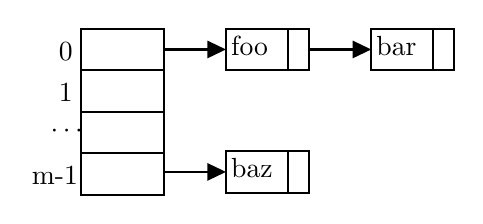
\begin{tikzpicture}[x=0.75pt,y=0.75pt,yscale=-1,xscale=1]
		%uncomment if require: \path (0,300); %set diagram left start at 0, and has height of 300

		%Shape: Rectangle [id:dp9579578997678553] 
		\draw   (70,100) -- (110,100) -- (110,120) -- (70,120) -- cycle ;
		%Shape: Rectangle [id:dp027628855530104857] 
		\draw   (70,80) -- (110,80) -- (110,100) -- (70,100) -- cycle ;
		%Shape: Rectangle [id:dp8143559001814539] 
		\draw   (70,140) -- (110,140) -- (110,160) -- (70,160) -- cycle ;
		%Shape: Rectangle [id:dp38276393364199424] 
		\draw   (70,120) -- (110,120) -- (110,140) -- (70,140) -- cycle ;
		%Straight Lines [id:da801581038753237] 
		\draw    (110,90) -- (137,90) ;
		\draw [shift={(140,90)}, rotate = 180] [fill={rgb, 255:red, 0; green, 0; blue, 0 }  ][line width=0.08]  [draw opacity=0] (8.93,-4.29) -- (0,0) -- (8.93,4.29) -- cycle    ;
		%Shape: Rectangle [id:dp3050844046907898] 
		\draw   (140,80) -- (180,80) -- (180,100) -- (140,100) -- cycle ;
		%Shape: Rectangle [id:dp41513696416167833] 
		\draw   (170,80) -- (180,80) -- (180,100) -- (170,100) -- cycle ;

		%Shape: Rectangle [id:dp43239961582118536] 
		\draw   (210,80) -- (250,80) -- (250,100) -- (210,100) -- cycle ;
		%Shape: Rectangle [id:dp38503115889664563] 
		\draw   (240,80) -- (250,80) -- (250,100) -- (240,100) -- cycle ;

		%Straight Lines [id:da3303160944704562] 
		\draw    (180,90) -- (207,90) ;
		\draw [shift={(210,90)}, rotate = 180] [fill={rgb, 255:red, 0; green, 0; blue, 0 }  ][line width=0.08]  [draw opacity=0] (8.93,-4.29) -- (0,0) -- (8.93,4.29) -- cycle    ;
		%Straight Lines [id:da047149376903893425] 
		\draw    (110,149) -- (137,149) ;
		\draw [shift={(140,149)}, rotate = 180] [fill={rgb, 255:red, 0; green, 0; blue, 0 }  ][line width=0.08]  [draw opacity=0] (8.93,-4.29) -- (0,0) -- (8.93,4.29) -- cycle    ;
		%Shape: Rectangle [id:dp591261104910037] 
		\draw   (140,139) -- (180,139) -- (180,159) -- (140,159) -- cycle ;
		%Shape: Rectangle [id:dp4443187367264515] 
		\draw   (170,139) -- (180,139) -- (180,159) -- (170,159) -- cycle ;


		% Text Node
		\draw (58,85) node [anchor=north west][inner sep=0.75pt]   [align=left] {0};
		% Text Node
		\draw (58,105) node [anchor=north west][inner sep=0.75pt]   [align=left] {1};
		% Text Node
		\draw (54,125) node [anchor=north west][inner sep=0.75pt]   [align=left] {$\displaystyle \cdots $};
		% Text Node
		\draw (45,145) node [anchor=north west][inner sep=0.75pt]   [align=left] {m-1};
		% Text Node
		\draw (141,82) node [anchor=north west][inner sep=0.75pt]   [align=left] {foo};
		% Text Node
		\draw (211,82) node [anchor=north west][inner sep=0.75pt]   [align=left] {bar};
		% Text Node
		\draw (141,141) node [anchor=north west][inner sep=0.75pt]   [align=left] {baz};
	\end{tikzpicture}
	\caption{Esempio di una tabella di hash con separate chaining.}
	\label{fig:hashtable_example}
\end{figure}

Possono accadere dei conflitti, ossia due stringhe $s_1$ e $s_2$ tali che
$h(s_1) = h(s_2)$; per ovviare a questo problema si descrive $M$ come una mappa di liste, ossia
ad un indice $h_1$ di $M$ corrisponde una lista di stringhe.

\subsubsection{Requisiti}
La tabella $M$ funziona con qualsiasi funzione di hash $h$ (anche $h(\cdot) = 0$),
ma l'efficienza di $M$ cambia al suo variare, fino al denegenerare in una lista.
Per far funzionare ``bene'' $M$ è necessario che
\begin{itemize}
	\setlength\itemsep{0pt}
	\item $h$ sia veloce da calcolare; e
	\item $h$ divida l'universo $U$ in \textit{buckets} in modo tale che le
	      controimmagini siano più o meno \textit{grandi uguali}.
	      In altri termini, se guardiamo $\Sigma^*$ e guardiamo come
	      $h$ ne partiziona gli elementi, vorremmo che i blocchi (o bucket)
	      della partizione siano più o meno grandi uguali e non ci sia
	      qualche blocco che contiene molti più elementi degli
	      altri.
	      % disegno pagina 1 15-12-2021 buckets nell'universo. 
\end{itemize}
Questi requisiti sono esprimibili formalmente ovviamente, ma solitamente oltre
a questi requisiti di base ve ne sono altri che dipendono dall'utilizzo
che si vuole fare della funzione; nel nostro caso, facciamo le seguenti
assunzioni: la prima, chiamata \textit{full randomness assumption},
è che possiamo estrarre uniformemente una funzione $h$ dall'insieme $\mathcal{H}_{U,m}$.

La seconda è che $h$ sia calcolabile in tempo e spazio costante, inoltre occupa
spazio costante in termini di codice (non usa array arbitrariamente grandi, ...).
Questa assunzione è normalmente inattuabile: si pensi al caso in cui $U = \Sigma^*$:
si dovrebbero considerare tutte le possibili funzioni dalle stringhe ai naturali
minori di $m$, che sono infinite e tra le quali ce ne sono anche di non calcolabili.

\subsubsection{Rappresentazione}
Ciò che si può fare è invece considerare un universo limitato con un
upper bound dipendente da un qualche intero $k$.
Chiaramente si perde della `randomness', ma il vantaggio è che molto spesso
i risultati che si ottengono sotto l'assunzione di completa casualità si possono
portare anche sotto $U$ così definito, magari con qualche approssimazione.

Supponiamo quindi di avere $U = \Sigma^{\leq k}$; vogliamo scrivere delle
funzioni $h: U \rightarrow m$, alcune di esse possono essere descritte nel
seguente modo.
Si usa un array $\mathbf{p}$ chiamato \textit{array dei pesi} contenente $k$ valori,
inizializzandolo a valori pseudocasuali nell'insieme $\{0, \cdots, m-1\}$.
Quando si vuole calcolare l'hash di una stringa $s = "foo"$ si considera il valore
di ogni lettera della stringa e si moltiplica per il peso di quel carattere
in senso posizionale, ossia il primo peso è associato al primo carattere della stringa,
il secondo peso al secondo carattere e così via; quindi si sommano i risultati e
si computa il modulo $m$. Per esempio, se
$$
	a = 0, b = 1, c = 2, \cdots, f = 5, \cdots, o = 14, \cdots
$$
e
$$
	\mathbf{p} = [15, 86, 90, \cdots]
$$
Il calcolo dell'hash è
$$
	h("foo") = ((5 * 15) + (14 * 86) + (14*90)) \mod m
$$
ottendo un valore che si calcola in un tempo lineare nella lunghezza della stringa
diverso per ogni possibile scelta dei pesi. Cioè, non stiamo
scegliendo tra tutte le possibili funzioni di hash, bensì scegliamo tra le funzioni
di hash caratterizzabili dal vettore $\mathbf{p}$, ossia in $m^k$ modi.
Queste funzioni non occupano molto spazio e si calcolano in un tempo non
costante ma logaritmico nella dimensione dell'universo.

\subsection{Relazione con i grafi}
\subsubsection{Sequenza di peeling di un grafo}
Si supponga di avere un grafo $G = (V,E)$ non orientato. Una \textbf{sequenza di peeling} è
una sequenza di coppie di archi e vertici in cui appaiono tutti i lati e uno dei
due vertici incidenti a tale lato. Ogni vertice che appare è chiamato \textit{hinge}
della sequenza. La sequenza deve essere tale per cui nessun vertice hinge $x_i$
è apparso nei lati che precedono $i$.

\begin{figure}[htpb]
	\begin{center}
		\begin{subfigure}[b]{0.45\textwidth}
			\begin{center}
				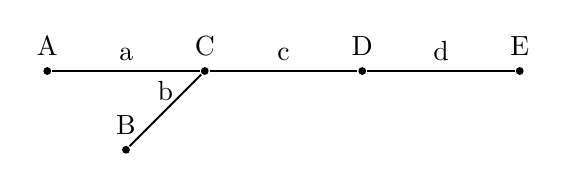
\begin{tikzpicture}
					\node [circle,fill,label=above:{A},inner sep=1pt](A) at (0,0) {};
					\node [circle,fill,label=above:{B},inner sep=1pt](B) at (1,-1) {};
					\node [circle,fill,label=above:{C},inner sep=1pt](C) at (2,0) {};
					\node [circle,fill,label=above:{D},inner sep=1pt](D) at (4,0) {};
					\node [circle,fill,label=above:{E},inner sep=1pt](E) at (6,0) {};

					\draw (A) -- (C) node [midway,above] {a};
					\draw (B) -- (C) node [midway,above] {b};
					\draw (C) -- (D) node [midway,above] {c};
					\draw (D) -- (E) node [midway,above] {d};
				\end{tikzpicture}

			\end{center}
		\end{subfigure}
		\begin{subfigure}[b]{0.45\textwidth}
			\begin{center}
				\begin{align*}
					a & = \{(A, C), A\} \\
					b & = \{(B, C), B\} \\
					c & = \{(C, D), D\} \\
					d & = \{(D, E), E\}
				\end{align*}
			\end{center}
		\end{subfigure}
	\end{center}
	\caption{Un grafo e una sequenza di peeling valida.}%
	\label{fig:example_peeling}
\end{figure}

Prendendo come esempio il grafo in \cref{fig:example_peeling}, per verificare una
sequenza di peeling si deve innanzitutto verificare che tutti i lati
appaiano nella sequenza; quindi, si verifica che ogni vertice non sia mai
comparso prima: per esempio, avendo scelto il lato $(A,B)$ invece di $(A,C)$,
non si sarebbe potuto scegliere il vertice $B$ da associare al lato $(B,C)$.

Non tutti i grafi ammettono una sequenza di peeling:
\begin{theorem}
	Un grafo $G$ ammette una sequenza di peeling se e solo se è aciclico.
\end{theorem}
\begin{proof}

	$\implies$ Per assurdo, si supponga che
	$\langle\{e_0, x_0\}, \cdots, \{e_{m-1}, x_{m-1}\}\rangle$
	sia una sequenza di peeling e che esista un ciclo sui vertici
	$y_1, y_2, \cdots, y_k$ e i relativi lati $\{y_1, y_2\}, \cdots, \{y_{k-1}, y_k\}$.
	Sia $\bar{i}$ l'indice massimo della sequenza del ciclo.
	Inserendo tutti i lati del ciclo nella sequenza, quando si arriva ad
	inserire l'ultimo lato del ciclo, non ci sarà modo di scegliere un nodo
	che ancora non appare nella sequenza.

	$\impliedby$ Per induzione su $|E|$. Omessa.
	%(esercizio). Hint: si parte dai lati più esterni. 
\end{proof}

\subsubsection{Ipergrafi}
Vogliamo ora generalizzare la nozione di sequenza di peeling agli ipergrafi.

\paragraph{Definizione}
Un $r$-ipergrafo è $G = (V, E)$ di vertici e \textit{iperlati} dove ogni iperlato è un
insieme di $r$ vertici, ossia $E \subseteq {V \choose r}$. Un esempio è
in \cref{fig:example:hypergraph}.

\begin{figure}[htpb]
	\begin{center}
		\begin{tikzpicture}[scale=1, transform shape]
			\node (f) at (0,0) {$F$};
			\node (g) at (1,0) {$G$};
			\node (e) at (2,0) {$E$};
			\node (d) at (2,1) {$D$};
			\node (a) at (2,2) {$A$};
			\node (b) at (3,2) {$B$};

			\node [draw, rounded corners,inner sep=0pt,fit=(f) (g)] {};
			\node [draw, dashed, rounded corners,inner sep=5pt,fit=(g) (e)] {};
			\node [draw, rounded corners,inner sep=0pt,fit=(a) (d) (e)] {};
			\node [draw, dashed, rounded corners,inner sep=5pt,fit=(a) (b) (d)] (fd){};
		\end{tikzpicture}
	\end{center}
	\caption{Esempio di ipergrafo.}%
	\label{fig:example:hypergraph}
\end{figure}

Non esiste una nozione di aciclicità per ipergrafi, mentre esiste una nozione di
sequenza di peeling: una sequenza di peeling per un $r$-ipergrafo è una sequenza
dei suoi iperlati ai quali si associa un hinge in modo tale che non sia mai apparso
negli iperlati precedenti.
Per questo motivo non si generalizza la nozione di aciclicità bensì quella di sequenza di peeling;
si dice che un ipergrafo è aciclico se e solo se ammette una sequenza di peeling.


\subsection{Tecnica MWHC}
\subsubsection{Funzioni statiche}
Il nostro obiettivo è memorizzare funzioni statiche.
Dato un universo $U$, un sottoinsieme fissato $X \subseteq U$ e $r \in \mathbb{N}$
vogliamo memorizzare una funzione
$$
	f: X \rightarrow 2^r
$$
di nuovo, si immagini $U$ come l'insieme dei caratteri ASCII;
una funzione $f$ può essere come quella in \cref{tab:example:static_func},
in cui $X$ è l'insieme di quelle tre stringhe: a noi non interessa
memorizzare stringhe diverse da quelle.

\begin{table}[htpb]
	\begin{tabular}{c|c c}
		x              & $f(x)$          &    \\
		\hline                                \\
		Paolo Boldi    & \texttt{00111}  & 7  \\
		Anna Zuppi     & \texttt{101000} & 20 \\
		Giovanni Galli & \texttt{101110} & 23
	\end{tabular}
	\centering
	\caption{Esempio di funzione statica.}
	\label{tab:example:static_func}
\end{table}

Memorizzare una funzione significa che vogliamo ricavare una struttura
dati $D$ tale che permette di valutare un input in modo da ottenere
il valore di $f(x)$ ossia, per esempio, $"Paolo Boldi" \mapsto 00111$ e così via, mentre
il comportamento inteso per gli input non appartenenti all'insieme $X$
che vogliamo memorizzare è irrilevante.
La funzione $f$ si definisce \textit{statica} poiché è paragonabile
alla struttura \textit{dizionario} nei linguaggi di programmazione come
Python, benché questa struttura sia immodificabile e
non ci sia modo di sapere se una certa chiave è presente o meno.

\subsubsection{Rappresentazione}
Per costruire una rappresentazione succinta si utilizza la tecnica
MWHC\footnote{Majewski, Worwald, Havas, Czech}.
Inizialmente si fissa un $m$ intero e si scelgono uniformemente due funzioni hash
$$
	h_1, h_2 : U \rightarrow m
$$
Assumiamo che $\forall x \in X ~ h_1(x) \neq h_2(x)$.
Costruiamo un grafo i cui vertici sono i numeri $0, \cdots, m-1$ e i lati
corrispondono agli elementi dell'insieme $X$, con l'idea che alla chiave $x$
corrisponde il lato $(h_1(x), h_2(x))$.

Seguendo l'esempio in \cref{tab:example:static_func}, immaginiamo che
le due funzioni calcolino l'hash delle stringhe in $X$ come descritto
in \cref{tab:static_hashes}, supponendo $m = 17$ e $r = 5$. 
Si può ora costruire un grafo costruito
come in \cref{fig:static_graph}: grazie all'assunzione precedente,
ossia la differenza dei due hash per ogni chiave, sappiamo che nel
grafo non vi sono cappi. In caso accada, si generano due nuove
funzioni $h_1$ e $h_2$. Inoltre, vogliamo che il grafo sia
aciclico e che a nessun lato corrispondano due o più chiavi diverse: anche
in questi casi si possono generare due nuove funzioni hash.

\begin{table}[htpb]
	\begin{tabular}{c | c | c}
		x              & $h_1(x)$ & $h_2(x)$ \\
		\hline                               \\
		Paolo Boldi    & 3        & 7        \\
		Anna Zuppi     & 14       & 13       \\
		Giovanni Galli & 13       & 2
	\end{tabular}
	\centering
	\caption{Calcolo di $h_1$ e $h_2$ sulle stringhe nell'insieme $X$.}
	\label{tab:static_hashes}
\end{table}
\begin{figure}[htpb]
	\begin{center}
		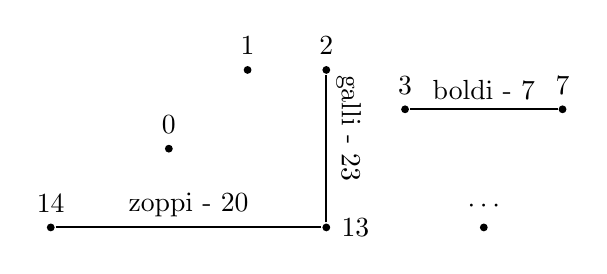
\begin{tikzpicture}
			\node [circle,fill,label=above:{0},inner sep=1pt](0) at (0,0) {};
			\node [circle,fill,label=above:{1},inner sep=1pt](1) at (1,1) {};
			\node [circle,fill,label=above:{2},inner sep=1pt](2) at (2,1) {};
			\node [circle,fill,label=above:{3},inner sep=1pt](3) at (3,0.5) {};
			\node [circle,fill,label=above:{7},inner sep=1pt](7) at (5,0.5) {};
			\node [circle,fill,label=right:{13},inner sep=1pt](13) at (2,-1) {};
			\node [circle,fill,label=above:{14},inner sep=1pt](14) at (-1.5,-1) {};
			\node [circle,fill,label=above:{$\cdots$},inner sep=1pt](d) at (4,-1) {};

			\draw (14) -- (13) node [midway,above] {zoppi - $20$};
			\draw (13) -- (2) node [midway,above, label={[rotate=-90]above:{galli - $23$}}] {};
			\draw (3) -- (7) node [midway,above] {boldi - $7$};
		\end{tikzpicture}

	\end{center}
	\caption{Grafo associato per la costruzione di una struttura per funzioni statiche.}%
	\label{fig:static_graph}
\end{figure}
Trasformeremo ora il grafo in un sistema di equazioni: ogni vertice è una variabile $w_0, w_1, \cdots, w_{m-1}$ e ad ogni lato corrisponde
l'equazione
$$
	\forall x \in X ~~ (w_{h_1(x)} + w_{h_2(x)}) \mod 2^r = f(x)
$$
Se il grafo è aciclico (che è un'assunzione) il sistema è risolvibile. 
L'esistenza di una sequenza di peeling (che esiste se e solo se il grafo è aciclico) significa 
che si possono ordinare le equazioni in modo che una delle due variabili non sia mai 
comparsa prima: questo significa che la soluzione si può trovare ordinando le equazioni
e assegnando il valore che rende vera l'equazione alla variabile che non è ancora apparsa. 
Quindi, per esempio
$$
\begin{cases}
    (w_{14} + w_{13}) \mod 2^5 = 20 \\
    (w_{2} + w_{13}) \mod 2^5 = 23 \\
    (w_{3} + w_{7}) \mod 2^5 = 7 \\
\end{cases}
$$
Usando come hinge $w_{14} = 20$, $w_{2} = 23$ e $w_{7} = 7$ si risolve il sistema. 

\subsubsection{Implementazione}
Una volta memorizzate le soluzioni $w_i$ del sistema in un vettore $\mathbf{w}$, 
si può calcolare $f(x)$ per ogni $x \in X$ come 
$$
f(x) = (w_{h_1(x)} + w_{h_2(x)}) \mod 2^m 
$$
Bisogna però decidere la grandezza di $m$, ossia il numero di vertici (o il numero di bucket, o il numero 
massimo che può risultare da un hash): è facile vedere che se $m$ è ``troppo piccolo'' è molto imporbabile 
che riescano a soddisfare le condizioni, ossia si troveranno cicli, collisioni e così via. Se si 
sceglie ``troppo grande'', la struttura che si memorizza occupa molto spazio. 
Precisamente, questo tradeoff dipende da quanto è probabile che il grafo generato sia aciclico. 
\begin{theorem}
    Se $m > (2.09 \cdot |X|)$, il grafo è ``quasi sempre'' aciclico. Il numero atteso di tentativi 
    di generazione di coppie di funzioni hash è circa $2$.
\end{theorem}
\begin{proof}
    Omessa.
\end{proof}

Naturalmente si può anche calcolare la funzione di un qualcosa che non è tra gli input desiderati e 
qualcosa verrà prodotto, ma non avrà un senso ben inteso. 

\subsubsection{Spazio}
Il vettore che dobbiamo memorizzare ha $m$ elementi, ognuno dei quali contiene $r$ bit: in tutto, 
il vettore occupa spazio $m\cdot r$ bit. Definendo $|X| = n$, dal teorema precedente si ha 
$m\cdot r \geq 2.09nr$; lo spazio totale si trova aggiungendo lo spazio per memorizzare 
le funzioni di hash $h_1$ e $h_2$.  

Tutto questo processo può essere eseguito non solo per i grafi (costruiti con $2$ funzioni hash)
ma anche per gli ipergrafi, costruendo un $r$-ipergrafo utilizzando $r$ funzioni hash. Ci si può 
quindi chiedere quale sia la costante che rende ipergrafi con $r > 2$ ``quasi sempre'' aciclici: 
\begin{theorem}
    Per ogni $k$-ipergrafo esiste una costante $\gamma_k$ tale che se $m > \gamma_k n$ allora 
    l'ipergrafo ammette quasi sempre una sequenza di peeling. 
\end{theorem}
\begin{proof}
    Omessa.
\end{proof}

In effetti, le costanti $\gamma_k$ hanno un minimo in $k = 3$: il meglio che si può 
ottenere è quindi utilizzando $3$ funzioni di hash. Il numero di bit che consuma 
$\mathbf{w}$ è quindi $1.23nr$ bit.  

\begin{table}[htpb]
    \centering
    \begin{tabular}{c|c}
	 $k$ &  $\gamma_k$ \\ 
	 \hline 
	 2 & 2.09 \\
	 3 & 1.23 \\
	 $\cdots$ & > 1.23 $\cdots$
    \end{tabular}
    \caption{Costanti $\gamma_k$ per $k$-ipergrafi.}
    \label{tab:gamma_k_hypergraph}
\end{table}

\subsubsection{Lower bound}
Per capire che tipo di struttura stiamo costruendo, dobbiamo calcolare l'information-theoretical 
lower bound. Stiamo memorizzando una funzione da un insieme $X$ fissato ad un insieme $2^r$.  
Le funzioni di questo tipo sono ${2^{r}}^{|X|} = 2^{r|X|} = 2^{rn}$, definendo come prima $|X| = n$. 
Quindi, l'information-theoretical lower bound è 
$$
Z_n = \log_2(2^{rn}) = rn \text{ bit}
$$
e la struttura che abbiamo descritto occupa 
$$
D_n = 1.23nr = O(Z_n) \text{ bit}
$$
pertanto la struttura è compatta.

\subsubsection{Struttura compressa}
Si può osservare che nel vettore $\mathbf{w}$ molte entry sono uguali a $0$: il numero 
di entry diverse da zero è pari al numero di hinge nella sequenza di peeling 
che risolve il sistema generato dal grafo, quindi $\mathbf{w}$ che (assumendo 
l'utlizzo di $3$ funzioni di hash) ha esattamente $m = 1.23n$ elementi, al più
$n$ elementi sono non nulli. 

Quindi, si possono memorizzare unicamente gli elementi non nulli in $\tilde{\mathbf{w}}$ 
utilizzando un ulteriore array $\mathbf{b}$ di $m$ bit tale che 
$$
\mathbf{b}[i] = \begin{cases}
    1 & \mathbf{w}[i] \neq 0 \\
    0 & \mathbf{w}[i] = 0
\end{cases}
$$
definendo quindi il vettore 
$$
\mathbf{w}[i] = \begin{cases}
    0 & \mathbf{b}[i] = 0 \\
    \tilde{\mathbf{w}}[\mathbf{rank_b}[i]] & \mathbf{b}[i] = 1
\end{cases}
$$
In questo modo, la struttura (che è comunque compatta) in totale occupa 
$$
D_n = nr + m = nr + 1.23n = (r + 1.23) n \text{ bit}
$$
e si ha quindi 
$$
(r + 1.23 ) n < 1.23rn \implies (r + 1.23) < 1.23r  \implies r > 5
$$

\noindent
Inizialmente, la tecnica MWHC era stata pensata per un uso ben più specifico, 
ossia memorizzare una funziona di hash minimale perfetta, ossia una funzione
che mappa $n$ chiavi in $n$ bucket privi di collisioni. 
Tuttavia questa tecnica è abbastanza generale da memorizzare qualsiasi funzione e 
si può utilizzare questa tecnica come intesa inizialmente semplicemente associando 
$f(x)$ diversi da $0$ a $n-1$ per ogni elemento di $X$. 
